\documentclass[a4paper,13pt,twoside]{report}

% ===================== GÓI CƠ BẢN =====================
\usepackage{scrextend}
\changefontsizes{13pt}
\usepackage[utf8]{inputenc}
\usepackage[T5]{fontenc}
\usepackage[vietnamese]{babel}
\usepackage[top=2cm,bottom=2cm,inner=3.5cm,outer=2.5cm]{geometry}
\usepackage{times}
\usepackage{setspace}
\usepackage{indentfirst}
\usepackage{graphicx}
\usepackage{float}
\usepackage{array}
\usepackage{enumitem}
\usepackage{amsmath,amssymb}
\usepackage{xcolor}
\usepackage{xurl}
\usepackage{hyperref}
\usepackage{titlesec}
\usepackage{titletoc}
\usepackage{fancyhdr}
\usepackage{caption}
\usepackage{subcaption}
\captionsetup{skip=6pt}
\usepackage{placeins}
\usepackage{booktabs}
\usepackage{longtable}
\usepackage{tabularx}
\usepackage{makecell}
\usepackage{microtype}
\usepackage{ragged2e}
\usepackage{tikz}
\usetikzlibrary{arrows.meta,positioning,shapes.geometric}
\newcolumntype{R}[1]{>{\RaggedLeft\arraybackslash}p{#1}}

% ===================== THIẾT LẬP CHUNG =====================
\onehalfspacing
\raggedbottom
\setlength{\parindent}{15pt}
\setlength{\parskip}{6pt}
\sloppy
\justifying
\hypersetup{
    pdfborder={0 0 0},
    pdftitle={HỆ THỐNG VOICEBOT TƯ VẤN DINH DƯỠNG THỜI GIAN THỰC DỰA TRÊN AI HỘI THOẠI},
    pdfauthor={Trần Quang Minh}
}

\def\TITLE{HỆ THỐNG VOICEBOT TƯ VẤN DINH DƯỠNG THỜI GIAN THỰC DỰA TRÊN AI HỘI THOẠI}
\def\TITLELINEONE{HỆ THỐNG VOICEBOT TƯ VẤN}
\def\TITLELINETWO{DINH DƯỠNG THỜI GIAN THỰC}
\def\TITLELINETHREE{DỰA TRÊN AI HỘI THOẠI}
\def\AUTHOR{TRẦN QUANG MINH}
\def\STUDENTID{minh.tq225047@sis.hust.edu.vn}
\def\PROGRAM{Chương trình đào tạo: Khoa học máy tính}
\def\FACULTY{Khoa học máy tính}
\def\SCHOOL{Công nghệ thông tin và Truyền thông}
\def\UNIVERSITY{ĐẠI HỌC BÁCH KHOA HÀ NỘI}
\def\SUPERVISOR{TS. Nguyễn Thị Thu Trang}

\titleformat{\chapter}[hang]{\centering\bfseries}{CHƯƠNG \thechapter.\ }{0pt}{}
\titlespacing*{\chapter}{0pt}{-20pt}{20pt}
\titleformat{\section}[hang]{\bfseries}{\thechapter.\arabic{section}\quad}{0pt}{}
\titleformat{\subsection}[hang]{\bfseries}{\thechapter.\arabic{section}.\arabic{subsection}\quad}{0pt}{}
\setcounter{secnumdepth}{3}
\setcounter{tocdepth}{2}

\pagestyle{fancy}
\fancyhf{}
\setlength{\headheight}{18pt}
\fancyhead[LE]{\leftmark}
\fancyhead[RO]{\leftmark}
\fancyfoot[RE]{\thepage}
\fancyfoot[LO]{\thepage}
\renewcommand{\headrulewidth}{0.4pt}
\fancypagestyle{plain}{
    \fancyhf{}
    \fancyfoot[RE]{\thepage}
    \fancyfoot[LO]{\thepage}
    \renewcommand{\headrulewidth}{0pt}
}
\makeatletter
\setlength{\@fptop}{0pt}
\setlength{\@fpsep}{10pt plus 1fil}
\setlength{\@fpbot}{0pt plus 1fil}
\makeatother

% ===================== TÀI LIỆU =====================
\begin{document}

% ===================== BÌA =====================
\begin{titlepage}
    \thispagestyle{empty}
    \begin{center}
        {\textbf{\large \UNIVERSITY}}\\[3.4cm]

        {\textbf{\huge ĐỒ ÁN TỐT NGHIỆP}}\\[0.9cm]
        {\textbf{\Large \TITLELINEONE}}\\[0.25cm]
        {\textbf{\Large \TITLELINETWO}}\\[0.25cm]
        {\textbf{\Large \TITLELINETHREE}}\\[0.9cm]

        {\textbf{\large \AUTHOR}}\\[-0.05cm]
        {\large \STUDENTID}\\[0.5cm]

        {\textbf{\large \PROGRAM}}

        \vspace{3.2cm}

        {\large
            \begin{tabular}{@{}ll@{}}
                \textbf{Giảng viên hướng dẫn:} & \SUPERVISOR \\[0.5cm]
                \textbf{Khoa:}                 & \FACULTY    \\[0.5cm]
                \textbf{Trường:}               & \SCHOOL     \\[4.0cm]
                \multicolumn{2}{c}{\textbf{HÀ NỘI, 06/2026}}
            \end{tabular}
        }
    \end{center}
\end{titlepage}

% ===================== BÌA LÓT =====================
\begin{titlepage}
    \thispagestyle{empty}
    \begin{center}
        {\textbf{\large \UNIVERSITY}}\\[3.4cm]

        {\textbf{\huge ĐỒ ÁN TỐT NGHIỆP}}\\[0.9cm]
        {\textbf{\Large \TITLELINEONE}}\\[0.25cm]
        {\textbf{\Large \TITLELINETWO}}\\[0.25cm]
        {\textbf{\Large \TITLELINETHREE}}\\[0.9cm]

        {\textbf{\large \AUTHOR}}\\[-0.05cm]
        {\large \STUDENTID}\\[0.5cm]

        {\textbf{\large \PROGRAM}}

        \vspace{2.4cm}

        {\large
            \begin{tabular}{@{}ll@{}}
                \textbf{Giảng viên hướng dẫn:} & \SUPERVISOR \\[0.5cm]
                \textbf{Khoa:}                 & \FACULTY    \\[0.5cm]
                \textbf{Trường:}               & \SCHOOL     \\[3.5cm]
                \multicolumn{2}{c}{\textbf{HÀ NỘI, 06/2026}}
            \end{tabular}
        }
    \end{center}
\end{titlepage}

\justifying

\pagenumbering{roman}

% ===================== LỜI CẢM ƠN =====================
\chapter*{}
\addcontentsline{toc}{chapter}{LỜI CẢM ƠN}
\vspace*{-1.8cm}
\begin{center}
    {\textbf{\LARGE LỜI CẢM ƠN}}
\end{center}
\vspace{1.0cm}

Trước hết, em xin bày tỏ lòng biết ơn sâu sắc tới TS.Nguyễn Thị Thu Trang, giảng viên hướng dẫn của em, vì sự quan tâm, định hướng và hỗ trợ tận tình trong suốt quá trình thực hiện đồ án. Những góp ý kịp thời, sự nghiêm túc trong chuyên môn và sự kiên nhẫn của cô đã giúp em nhìn nhận vấn đề rõ ràng hơn, điều chỉnh hướng nghiên cứu phù hợp hơn và hoàn thiện đồ án này.

Em xin gửi lời cảm ơn chân thành tới anh Nguyễn Hoàng Kỳ và team TTS đã dành thời gian hỗ trợ, chia sẻ kinh nghiệm kỹ thuật và tạo điều kiện để em tiếp cận, thử nghiệm và tích hợp các thành phần liên quan đến tổng hợp tiếng nói trong hệ thống. Những trao đổi thực tế trong quá trình làm việc đã giúp em hiểu rõ hơn các khó khăn khi đưa mô hình vào một pipeline chạy được, đặc biệt là các vấn đề về độ trễ, streaming và chất lượng âm thanh.

Em cũng xin cảm ơn các anh chị, bạn bè và đồng nghiệp trong môi trường học tập, nghiên cứu đã luôn hỗ trợ, trao đổi và đồng hành cùng em trong quá trình phát triển hệ thống. Sự giúp đỡ của mọi người không chỉ có ý nghĩa về mặt chuyên môn mà còn là nguồn động viên quan trọng để em duy trì tiến độ và hoàn thành đồ án.

Cuối cùng, em xin gửi lời cảm ơn sâu sắc tới gia đình và những người thân yêu đã luôn tin tưởng, động viên và là chỗ dựa tinh thần vững chắc cho em trong suốt quá trình học tập. Sự ủng hộ của mọi người là điều kiện quan trọng để em có thể hoàn thiện đồ án này.

\newpage

% ===================== TÓM TẮT =====================
\chapter*{}
\addcontentsline{toc}{chapter}{TÓM TẮT NỘI DUNG ĐỒ ÁN}
\vspace*{-1.8cm}
\begin{center}
    {\textbf{\LARGE TÓM TẮT NỘI DUNG ĐỒ ÁN}}
\end{center}
\vspace{1.0cm}

Hệ thống hỏi đáp qua tiếng nói đòi hỏi kết hợp liên tiếp nhiều thành phần: nhận dạng tiếng nói, truy xuất tri thức, sinh câu trả lời và tổng hợp tiếng nói. Chất lượng cuối cùng phụ thuộc đồng thời vào độ chính xác của transcript, mức phù hợp của ngữ cảnh truy xuất và độ trễ tích lũy trong toàn bộ pipeline.

Đồ án xây dựng hệ thống tư vấn dinh dưỡng qua tiếng nói tiếng Việt theo kiến trúc pipeline mô-đun gồm ASR, xử lý hội thoại dựa trên Retrieval-Augmented Generation và TTS. Kho tri thức gồm khoảng 1000 bài viết dinh dưỡng được truy xuất bằng mô hình nhúng tiếng Việt, xếp hạng lại bằng cross-encoder và đưa vào mô hình ngôn ngữ. Hệ thống sử dụng guardrail lọc câu hỏi ngoài phạm vi và kiểm tra mức đủ ngữ cảnh trước khi sinh câu trả lời.

Đóng góp chính là cơ chế streaming song song giữa sinh văn bản và tổng hợp tiếng nói, giúp rút ngắn thời gian chờ mà không thay đổi các mô hình nền. Kết quả thực nghiệm đạt faithfulness 0,7723 với cấu hình 15 đoạn ứng viên, chọn 5 đoạn; trung vị Time-to-First-Audio giảm từ 1523~ms xuống 747~ms khi dùng ngưỡng chia đoạn 40 ký tự. Các kết quả này cho thấy cách tổ chức pipeline ảnh hưởng trực tiếp đến khả năng cân bằng giữa độ tin cậy của câu trả lời và độ trễ cảm nhận.

\vspace{0.4cm}
\begin{flushright}
    Sinh viên thực hiện\\[0.1cm]
    
\includegraphics[width=4.5cm]{downl-removebg-preview.png}\\[-0.4cm]
    \textit{Trần Quang Minh}
\end{flushright}

\newpage
\renewcommand{\contentsname}{MỤC LỤC}
\tableofcontents
\newpage
\renewcommand{\listfigurename}{DANH MỤC HÌNH VẼ}
\begingroup
\renewcommand{\numberline}[1]{\makebox[2.8cm][l]{Hình~#1}}
\listoffigures
\endgroup
\newpage
\renewcommand{\listtablename}{DANH MỤC BẢNG BIỂU}
\begingroup
\renewcommand{\numberline}[1]{\makebox[2.8cm][l]{Bảng~#1}}
\listoftables
\endgroup
\newpage

\chapter*{}
\addcontentsline{toc}{chapter}{DANH MỤC THUẬT NGỮ VÀ TỪ VIẾT TẮT}
\vspace*{-1.8cm}
\begin{center}
    {\textbf{\Large DANH MỤC THUẬT NGỮ VÀ TỪ VIẾT TẮT}}
\end{center}
\vspace{0.5cm}

\begingroup
\small
\renewcommand{\arraystretch}{1.25}
\setlength{\LTleft}{0pt}
\setlength{\LTright}{0pt}
\begin{longtable}{|p{2.6cm}|p{11.2cm}|}
    \hline
    \textbf{Thuật ngữ} & \textbf{Ý nghĩa}                                                                  \\
    \hline
    \endfirsthead
    \hline
    \textbf{Thuật ngữ} & \textbf{Ý nghĩa}                                                                  \\
    \hline
    \endhead
    AI                 & Trí tuệ nhân tạo (Artificial Intelligence)                                        \\
    \hline
    API                & Giao diện lập trình ứng dụng (Application Programming Interface)                  \\
    \hline
    ASR                & Nhận dạng tiếng nói tự động (Automatic Speech Recognition)                        \\
    \hline
    CTC                & Phân loại thời gian kết nối (Connectionist Temporal Classification)               \\
    \hline
    CUDA               & Nền tảng tính toán song song của NVIDIA (Compute Unified Device Architecture)     \\
    \hline
    CPU                & Bộ xử lý trung tâm (Central Processing Unit)                                      \\
    \hline
    GPU                & Bộ xử lý đồ họa (Graphics Processing Unit)                                        \\
    \hline
    HNSW               & Cấu trúc đồ thị tìm kiếm láng giềng gần đúng (Hierarchical Navigable Small World) \\
    \hline
    HTTP               & Giao thức truyền siêu văn bản (Hypertext Transfer Protocol)                       \\
    \hline
    HyDE               & Truy xuất bằng tài liệu giả định (Hypothetical Document Embeddings)               \\
    \hline
    LLM                & Mô hình ngôn ngữ lớn (Large Language Model)                                       \\
    \hline
    MOS                & Điểm đánh giá chủ quan trung bình (Mean Opinion Score)                            \\
    \hline
    ONNX               & Định dạng trao đổi mô hình học máy (Open Neural Network Exchange)                 \\
    \hline
    PCM                & Mã hóa âm thanh dạng xung mã (Pulse-Code Modulation)                              \\
    \hline
    RAG                & Sinh câu trả lời tăng cường truy xuất (Retrieval-Augmented Generation)            \\
    \hline
    RAGAS              & Bộ công cụ đánh giá hệ thống RAG (Retrieval-Augmented Generation Assessment)      \\
    \hline
    RNN-T              & Mô hình chuyển đổi chuỗi RNN-T (Recurrent Neural Network Transducer)              \\
    \hline
    RTF                & Hệ số thời gian thực (Real-Time Factor)                                           \\
    \hline
    TTS                & Tổng hợp tiếng nói từ văn bản (Text-to-Speech)                                    \\
    \hline
    TTFA               & Thời gian tới âm thanh đầu tiên (Time-to-First-Audio)                             \\
    \hline
    TTFT               & Thời gian tới token đầu tiên (Time-to-First-Token)                                \\
    \hline
    TTL                & Thời gian tồn tại của dữ liệu hoặc cache (Time To Live)                           \\
    \hline
    URL                & Địa chỉ tài nguyên (Uniform Resource Locator)                                     \\
    \hline
    VAD                & Phát hiện hoạt động tiếng nói (Voice Activity Detection)                          \\
    \hline
    WER                & Tỷ lệ lỗi từ (Word Error Rate)                                                    \\
    \hline
\end{longtable}
\endgroup
\newpage

% ===================== NỘI DUNG CHÍNH =====================
\pagenumbering{arabic}

\chapter{GIỚI THIỆU BÀI TOÁN}

\section{Đặt vấn đề}

Nhu cầu tiếp cận thông tin và đặt câu hỏi tư vấn xuất hiện trong nhiều hoạt động hằng ngày. Thay vì tự tìm kiếm, đọc và tổng hợp từ nhiều tài liệu, người dùng mong muốn trình bày vấn đề bằng ngôn ngữ tự nhiên và nhận lại câu trả lời ngắn gọn, dễ hiểu. Hệ thống hỏi đáp tư vấn đáp ứng nhu cầu này bằng cách tiếp nhận câu hỏi, xác định nội dung người dùng quan tâm và cung cấp thông tin trong một phạm vi xác định. Dạng hệ thống này có thể được ứng dụng trong chăm sóc khách hàng, giáo dục, tổng đài tự động, trợ lý cá nhân và các hệ thống hỗ trợ tra cứu tri thức theo chủ đề.

Chatbot văn bản là hình thức phổ biến của hệ thống hỏi đáp tư vấn. Người dùng nhập câu hỏi trên website, ứng dụng di động hoặc nền tảng nhắn tin và nhận câu trả lời dưới dạng văn bản. Việc sử dụng mô hình ngôn ngữ lớn giúp chatbot hiểu nhiều cách diễn đạt và tạo phản hồi tự nhiên. Tuy nhiên, nếu chỉ dựa trên kiến thức được lưu trong tham số mô hình, câu trả lời có thể thiếu thông tin cập nhật, không phù hợp với phạm vi tư vấn hoặc chứa nội dung nghe hợp lý nhưng không có căn cứ rõ ràng. Retrieval-Augmented Generation khắc phục một phần hạn chế này bằng cách truy xuất các đoạn văn bản liên quan từ kho tri thức, đưa chúng vào ngữ cảnh của mô hình ngôn ngữ rồi mới sinh câu trả lời. Nhờ đó, phản hồi được định hướng bởi nguồn dữ liệu đã lựa chọn thay vì chỉ phụ thuộc vào kiến thức chung của mô hình.

Mặc dù thuận tiện, chatbot văn bản vẫn yêu cầu người dùng nhìn màn hình và thao tác bằng bàn phím hoặc màn hình cảm ứng. Điều này gây bất tiện đối với người có thị lực kém, người gặp khó khăn khi nhập liệu, trẻ nhỏ chưa biết chữ hoặc chưa nhập văn bản thành thạo, và các tình huống người dùng không thể sử dụng tay. Ví dụ, một người đang di chuyển bằng ô tô có thể muốn hỏi nhanh về chế độ ăn hoặc lựa chọn thực phẩm nhưng không nên nhập một câu hỏi dài trên thiết bị. Trong tổng đài tự động, trao đổi trực tiếp bằng tiếng nói cũng tự nhiên hơn so với yêu cầu người gọi chuyển sang giao diện văn bản. Vì vậy, tiếng nói là một kênh giao tiếp quan trọng để mở rộng khả năng tiếp cận của hệ thống hỏi đáp tư vấn.

Voicebot mở rộng hệ thống hỏi đáp tư vấn sang tương tác hai chiều bằng tiếng nói: người dùng đặt câu hỏi bằng tiếng nói và nhận lại câu trả lời dưới dạng âm thanh. Một lượt xử lý thường gồm nhận dạng tiếng nói để chuyển âm thanh thành transcript, xử lý hội thoại để hiểu câu hỏi và truy xuất tri thức, mô hình ngôn ngữ để sinh câu trả lời, sau đó tổng hợp tiếng nói để tạo âm thanh phản hồi. So với chatbot văn bản, cách tương tác này phù hợp hơn với tổng đài, trợ lý tiếng nói, người có hạn chế về thị giác hoặc người đang không rảnh tay. Tuy nhiên, nó cũng làm bài toán khó hơn vì chất lượng cuối cùng phụ thuộc vào sự phối hợp của nhiều mô-đun thay vì chỉ một mô hình sinh văn bản.

Thách thức đầu tiên của hệ thống hỏi đáp qua tiếng nói là độ chính xác. Sai số ở một bước có thể truyền sang các bước tiếp theo. Nếu nhận dạng tiếng nói sai một thuật ngữ quan trọng, truy vấn đưa vào hệ thống truy xuất có thể bị lệch, tài liệu được chọn có thể không còn phù hợp và câu trả lời cuối cùng sẽ không đúng nhu cầu của người dùng. Vì vậy, hệ thống cần kết hợp nhận dạng tiếng nói, chuẩn hóa truy vấn, truy xuất tri thức, mô hình xếp hạng lại và prompt có ngữ cảnh một cách nhất quán. Chất lượng câu trả lời không chỉ phụ thuộc vào mô hình ngôn ngữ mà còn phụ thuộc vào cách chọn tri thức đầu vào cho mô hình.

Thách thức thứ hai là độ trễ. Thời gian chờ của người dùng được tích lũy qua nhiều bước: nhận dạng tiếng nói, truy xuất, sinh câu trả lời và tổng hợp tiếng nói. Nếu các bước này hoạt động hoàn toàn tuần tự, hệ thống phải sinh xong toàn bộ văn bản và tổng hợp xong toàn bộ âm thanh trước khi người dùng nghe được phản hồi. Khoảng im lặng dài làm hội thoại thiếu tự nhiên, đặc biệt trong các ứng dụng cần tương tác nhanh. Do đó, một hệ thống hỏi đáp tư vấn qua tiếng nói cần lựa chọn các mô-đun ASR, LLM và TTS phù hợp với streaming, đồng thời tổ chức luồng xử lý để phần âm thanh đầu tiên được phát sớm nhất có thể.

Trong đồ án này, dinh dưỡng được lựa chọn làm chủ đề minh họa để xây dựng và đánh giá hệ thống. Đây là chủ đề gần gũi với đời sống, có nhu cầu tra cứu thường xuyên và có nhiều dạng câu hỏi khác nhau như lựa chọn thực phẩm, nhóm chất, vitamin, khoáng chất, kiểm soát cân nặng hoặc chế độ ăn cho từng nhóm đối tượng. Đồng thời, dinh dưỡng có liên quan đến sức khỏe nên câu trả lời cần thận trọng, dựa trên nguồn thông tin đã lựa chọn, giới hạn ở mức tham khảo và không trình bày như chẩn đoán hoặc chỉ định điều trị. Một nhiệm vụ của đồ án là tổng hợp khoảng 1000 bài viết dinh dưỡng từ các nguồn có tính chuyên môn để xây dựng kho tri thức phục vụ truy xuất.

Từ những vấn đề trên, đồ án hướng tới xây dựng một hệ thống hỏi đáp tư vấn tiếng Việt qua tương tác hai chiều bằng tiếng nói, lấy chủ đề dinh dưỡng làm trường hợp ứng dụng cụ thể. Hệ thống sử dụng RAG để tạo câu trả lời dựa trên kho tri thức, khảo sát và lựa chọn các mô-đun ASR, LLM và TTS phù hợp với yêu cầu streaming, đồng thời tổ chức cơ chế phối hợp giữa sinh văn bản và tổng hợp tiếng nói nhằm giảm thời gian chờ trước khi người dùng nghe được phản hồi đầu tiên.

\section{Mục tiêu và phạm vi}

Phạm vi của đồ án được giới hạn trong bài toán tư vấn dinh dưỡng bằng tiếng Việt qua kênh thoại. Về ngôn ngữ, hệ thống tập trung xử lý tiếng Việt ở cả đầu vào tiếng nói, câu hỏi văn bản trung gian và câu trả lời đầu ra. Về chủ đề, hệ thống chỉ xử lý các câu hỏi dinh dưỡng phổ biến như lựa chọn thực phẩm, chế độ ăn hằng ngày, vi chất, nhóm thực phẩm, kiểm soát cân nặng, dinh dưỡng cho phụ nữ mang thai, trẻ em, người cao tuổi và một số tình trạng sức khỏe thường gặp. Đồ án không đặt mục tiêu thay thế bác sĩ, chuyên gia dinh dưỡng hoặc hệ thống chẩn đoán y khoa.

Về kênh tương tác, đồ án tập trung vào voicebot thay vì chatbot văn bản thuần túy. Người dùng đặt câu hỏi bằng tiếng nói, hệ thống nhận dạng thành văn bản, truy xuất tri thức, sinh câu trả lời và phát lại bằng tiếng nói. Giao diện văn bản chỉ đóng vai trò hỗ trợ hiển thị nội dung nhận dạng và trạng thái xử lý; mục tiêu chính vẫn là trải nghiệm hội thoại bằng tiếng nói với độ trễ thấp.

Phạm vi nghiên cứu không bao gồm xây dựng mô hình ASR, LLM hoặc TTS từ đầu; đồ án lựa chọn và tích hợp các mô hình có sẵn, sau đó tập trung vào tổ chức pipeline, xây dựng kho tri thức, cải thiện truy xuất và tối ưu luồng phản hồi. Về dữ liệu, đồ án hướng tới một kho tri thức ban đầu ở quy mô tối thiểu khoảng 1000 bài viết dinh dưỡng từ các nguồn công khai có tính chuyên môn; các bài viết sau làm sạch được phân đoạn ở mức vài trăm ký tự để phục vụ truy xuất. Kết quả của hệ thống chỉ có vai trò cung cấp thông tin tham khảo ban đầu trong phạm vi kho tri thức đã xây dựng.

Trong phạm vi nêu trên, mục tiêu đầu tiên của đồ án là xây dựng được một nguyên mẫu có khả năng xử lý một lượt hỏi đáp hoàn chỉnh qua tiếng nói tiếng Việt thuộc chủ đề dinh dưỡng phổ biến. Người dùng có thể đặt câu hỏi bằng tiếng nói, hệ thống nhận dạng nội dung câu hỏi, tạo câu trả lời và phát lại phản hồi dưới dạng âm thanh.

Với kho tri thức được tổng hợp từ khoảng 1000 bài viết dinh dưỡng có tính chuyên môn, hệ thống cần truy xuất được các đoạn văn bản phù hợp để làm ngữ cảnh cho mô hình ngôn ngữ. Trên tập đánh giá của đồ án, câu trả lời cần bám vào ngữ cảnh truy xuất, hạn chế suy diễn ngoài tài liệu và đạt các chỉ số chất lượng ở mức chấp nhận được.

Trong môi trường thử nghiệm với các mô-đun ASR, LLM và TTS được lựa chọn sẵn, đồ án hướng tới giảm thời gian từ khi có câu hỏi đến khi người dùng nghe được phần âm thanh phản hồi đầu tiên. Chỉ số trọng tâm là Time-to-First-Audio; mục tiêu tương đối là đưa TTFA trung vị xuống khoảng dưới 1--1,5 giây trong các lượt hỏi đáp thử nghiệm.

Cuối cùng, khi hệ thống được triển khai theo các mô-đun tách biệt, bộ điều phối phiên cần bảo đảm audio, transcript, text stream và audio stream thuộc đúng phiên hội thoại. Hệ thống cũng cần duy trì lịch sử ngắn hạn, bản tóm tắt phiên và cache truy xuất để hỗ trợ câu hỏi nối tiếp hoặc câu hỏi lặp lại.

\section{Định hướng giải pháp}

Định hướng giải pháp của đồ án là xây dựng một pipeline tương tác hai chiều bằng tiếng nói cho tư vấn dinh dưỡng tiếng Việt. Audio được truyền từ giao diện người dùng tới hệ thống theo các khung ngắn để phục vụ phát hiện tiếng nói và xác định kết thúc lượt nói. Sau đó, mô-đun ASR tạo transcript cuối cùng cho lượt hội thoại; mô-đun xử lý hội thoại kiểm tra phạm vi câu hỏi, chuẩn hóa truy vấn, truy xuất tri thức và sinh câu trả lời; mô-đun TTS chuyển câu trả lời thành âm thanh để phát lại cho người dùng. Một bộ điều phối phiên liên kết các mô-đun và bảo đảm dữ liệu của từng lượt hỏi đáp được xử lý đúng phiên.

Để hạn chế việc mô hình ngôn ngữ trả lời chỉ dựa trên tri thức tham số, hệ thống sử dụng Retrieval-Augmented Generation. Kho bài viết dinh dưỡng sau khi làm sạch được phân đoạn, mã hóa thành vector embedding và lưu trong vector database. Với mỗi câu hỏi, hệ thống thực hiện truy xuất hai bước: lấy một tập văn bản ứng viên bằng tìm kiếm vector, sau đó dùng mô hình reranker để chọn một tập nhỏ hơn làm ngữ cảnh cho LLM. Trước bước sinh câu trả lời, lớp kiểm soát đầu vào dựa trên luật được sử dụng để phát hiện một số câu hỏi ngoài phạm vi hoặc có dấu hiệu rủi ro; kết quả truy xuất cũng được kiểm tra ở mức tối thiểu nhằm tránh trả lời chắc chắn khi không có đủ ngữ cảnh.

Đối với kênh thoại, độ trễ là vấn đề trung tâm của giải pháp. Nếu hệ thống xử lý tuần tự, người dùng phải chờ nhận dạng tiếng nói, truy xuất tài liệu, sinh toàn bộ câu trả lời và tổng hợp xong toàn bộ âm thanh rồi mới nghe được phản hồi. Vì vậy, đồ án định hướng tổ chức quá trình trả lời theo streaming: khi LLM sinh được một phần văn bản đủ điều kiện, phần văn bản đó được chuyển sớm sang TTS thay vì chờ toàn bộ câu trả lời hoàn tất. Chiến thuật phân đoạn văn bản dựa trên dấu câu và ranh giới từ được sử dụng để chia văn bản tại các vị trí tương đối tự nhiên, nhằm giảm Time-to-First-Audio nhưng vẫn hạn chế việc TTS đọc bị ngắt nhịp.

Về kiến trúc triển khai, các chức năng được tách thành các nhóm mô-đun chính gồm giao diện người dùng, bộ điều phối phiên, nhận dạng tiếng nói, xử lý hội thoại, tổng hợp tiếng nói, kho tri thức dạng vector và bộ nhớ phiên. Cách tổ chức này cho phép đo thời gian từng giai đoạn, thay thế mô hình độc lập và cô lập lỗi tốt hơn so với đặt toàn bộ pipeline trong một tiến trình. Các mô-đun phục vụ chung một luồng nghiệp vụ và được bộ điều phối phiên điều phối tập trung.

Để hiện thực định hướng trên, đồ án kết hợp các kỹ thuật nhận dạng và tổng hợp tiếng nói, mô hình ngôn ngữ lớn, Retrieval-Augmented Generation, truy xuất vector, reranking và xử lý dữ liệu dạng streaming. Các thành phần được lựa chọn và tổ chức nhằm bảo đảm câu trả lời dựa trên kho tri thức dinh dưỡng, đồng thời giảm thời gian chờ trước khi người dùng nghe được âm thanh phản hồi đầu tiên. Hiệu quả của giải pháp được xem xét trên cả chất lượng truy xuất, mức độ câu trả lời bám sát ngữ cảnh và độ trễ của pipeline.

\section{Cấu trúc đồ án}

Phần còn lại của báo cáo được tổ chức theo mạch từ cơ sở lý thuyết, giải pháp đề xuất, phát triển hệ thống, thực nghiệm đến kết luận. Chương 1 giới thiệu bối cảnh của bài toán hỏi đáp tư vấn dinh dưỡng qua kênh tiếng nói, phân tích nhu cầu sử dụng voicebot, các thách thức về độ chính xác và độ trễ, đồng thời xác định mục tiêu và phạm vi của đồ án.

Chương 2 trình bày các nền tảng lý thuyết cần thiết để xây dựng hệ thống, gồm nhận dạng tiếng nói, Retrieval-Augmented Generation, mô hình ngôn ngữ, truy xuất vector, reranking và tổng hợp tiếng nói. Chương này đóng vai trò giải thích các thành phần chính của pipeline trước khi đi vào thiết kế hệ thống cụ thể.

Chương 3 mô tả giải pháp đề xuất ở mức thiết kế, bao gồm kiến trúc hệ thống, vai trò của các mô-đun, cách tổ chức kho tri thức, bộ nhớ phiên và chiến thuật streaming để giảm thời gian phản hồi âm thanh đầu tiên. Ở chương này, các thành phần được trình bày theo chức năng thay vì tập trung vào tên công cụ triển khai.

Chương 4 trình bày quá trình phát triển hệ thống voicebot tư vấn dinh dưỡng. Nội dung chương này đi vào kiến trúc triển khai, các công nghệ và mô hình cụ thể được sử dụng, thiết kế giao diện, backend, cơ sở dữ liệu, cũng như quá trình xây dựng, tích hợp, đóng gói và kiểm thử hệ thống.

Chương 5 trình bày thực nghiệm và đánh giá. Chương này mô tả cách xây dựng kho tri thức và tập dữ liệu đánh giá, thiết lập thực nghiệm, các độ đo được sử dụng, sau đó lần lượt phân tích kết quả của TTS, RAG và ASR. Chương 6 tổng kết các đóng góp chính, nêu kết luận rút ra từ quá trình thực hiện và đề xuất các hướng phát triển tiếp theo.

\chapter{CƠ SỞ LÝ THUYẾT}

\section{Nhận dạng tiếng nói tự động}

\subsection{Bài toán và biểu diễn tín hiệu}

Nhận dạng tiếng nói tự động là bài toán chuyển tín hiệu âm thanh thành chuỗi ký hiệu ngôn ngữ tương ứng. Gọi \(X=(x_1,x_2,\ldots,x_T)\) là chuỗi đặc trưng âm học gồm \(T\) khung thời gian và \(Y=(y_1,y_2,\ldots,y_U)\) là chuỗi \(U\) token đầu ra. Trong thực tế, số khung âm học thường lớn hơn nhiều số token văn bản và ranh giới giữa từng đoạn âm thanh với từng token không được cung cấp sẵn. Mô hình vì vậy phải học đồng thời biểu diễn nội dung âm học, quan hệ ngữ cảnh và phép căn chỉnh giữa hai chuỗi có độ dài khác nhau \cite{rnnt}.

Waveform thô có tần số lấy mẫu cao và chứa nhiều dao động không thuận tiện để đưa trực tiếp vào mô hình nhận dạng. Một quy trình tiền xử lý phổ biến là chia tín hiệu thành các cửa sổ ngắn, thực hiện biến đổi Fourier thời gian ngắn, chiếu phổ công suất qua các bộ lọc trên thang Mel và lấy logarithm năng lượng. Với \(S_t(f)\) là phổ công suất của khung thứ \(t\) và \(H_m(f)\) là bộ lọc Mel thứ \(m\), đặc trưng log-Mel có thể biểu diễn khái quát như sau:

\begin{equation}
    x_{t,m}
    =
    \log\left(
    \sum_f S_t(f)H_m(f)+\epsilon
    \right),
\end{equation}

trong đó \(\epsilon\) là một hằng số nhỏ để tránh logarithm của 0. Cách biểu diễn này nén waveform thành chuỗi vector đặc trưng theo thời gian, đồng thời giữ lại phân bố năng lượng theo các dải tần có ý nghĩa đối với cảm nhận tiếng nói. Chẳng hạn, công trình Conformer sử dụng đặc trưng filterbank 80 chiều được tính trên cửa sổ 25 ms với bước dịch 10 ms \cite{conformer}. Các đặc trưng sau đó có thể được giảm tần suất khung trước khi đi qua encoder nhằm giảm độ dài chuỗi và chi phí tính toán.

\subsection{RNN-Transducer}

Recurrent Neural Network Transducer (RNN-T) là mô hình xác suất đầu cuối dành cho bài toán chuyển đổi chuỗi khi căn chỉnh giữa đầu vào và đầu ra chưa biết trước \cite{rnnt}. Không gian token đầu ra \(\mathcal{Y}\) được mở rộng bằng ký hiệu rỗng \(\varnothing\). Một chuỗi căn chỉnh \(a\) gồm các token của \(Y\) xen kẽ với các ký hiệu rỗng; khi loại bỏ toàn bộ ký hiệu rỗng khỏi \(a\), ta thu được chuỗi văn bản \(Y\). Xác suất của \(Y\) được tính bằng tổng xác suất của tất cả các căn chỉnh hợp lệ:

\begin{equation}
    P(Y\mid X)
    =
    \sum_{a\in\mathcal{B}^{-1}(Y)}
    P(a\mid X),
\end{equation}

trong đó \(\mathcal{B}\) là phép loại bỏ ký hiệu rỗng. Nhờ lấy tổng trên các đường căn chỉnh, mô hình không yêu cầu dữ liệu huấn luyện phải chỉ rõ token nào tương ứng với khung âm thanh nào.

RNN-T gồm ba thành phần. Encoder âm học chuyển chuỗi đặc trưng \(X\) thành các biểu diễn \(h_t^{\mathrm{enc}}\), trong đó mỗi vector mô tả nội dung âm học tại thời điểm \(t\) cùng ngữ cảnh xung quanh. Prediction network nhận các token đã được sinh trước đó và tạo biểu diễn \(h_u^{\mathrm{pred}}\), đóng vai trò tương tự một mô hình ngôn ngữ phụ thuộc vào tiền tố đầu ra. Joiner kết hợp hai nguồn biểu diễn để tạo phân phối xác suất trên tập token mở rộng:

\begin{equation}
    P(k\mid t,u)
    =
    \operatorname{softmax}
    \left(
    W_j\,
    \phi\left(
        W_e h_t^{\mathrm{enc}}
        +
        W_p h_u^{\mathrm{pred}}
        +b
        \right)
    \right)_k,
\end{equation}

trong đó \(k\in\mathcal{Y}\cup\{\varnothing\}\), \(\phi\) là hàm kích hoạt và \(t,u\) lần lượt biểu diễn vị trí trên chuỗi âm học và chuỗi đầu ra. Nếu joiner dự đoán ký hiệu rỗng, quá trình giải mã chuyển sang khung âm học tiếp theo nhưng không bổ sung token văn bản. Nếu một token khác rỗng được dự đoán, token đó được thêm vào đầu ra và trạng thái của prediction network được cập nhật trong khi vị trí âm học có thể được giữ nguyên. Hai loại chuyển trạng thái này tạo thành một lưới kích thước xấp xỉ \(T\times U\), trên đó mỗi đường đi hợp lệ tương ứng với một phép căn chỉnh.

Hình~\ref{fig:rnnt-alignment-lattice} minh họa lưới xác suất của RNN-T. Trục ngang biểu diễn tiến trình theo chuỗi âm học, còn trục dọc biểu diễn số token đã được phát ra. Mũi tên ngang tương ứng với việc sinh ký hiệu rỗng để chuyển sang thời điểm âm học tiếp theo; mũi tên dọc tương ứng với việc sinh thêm một token đầu ra. Đường màu đỏ là một trong nhiều phép căn chỉnh có thể tạo ra cùng chuỗi tham chiếu.

\begin{figure}[H]
    \centering
    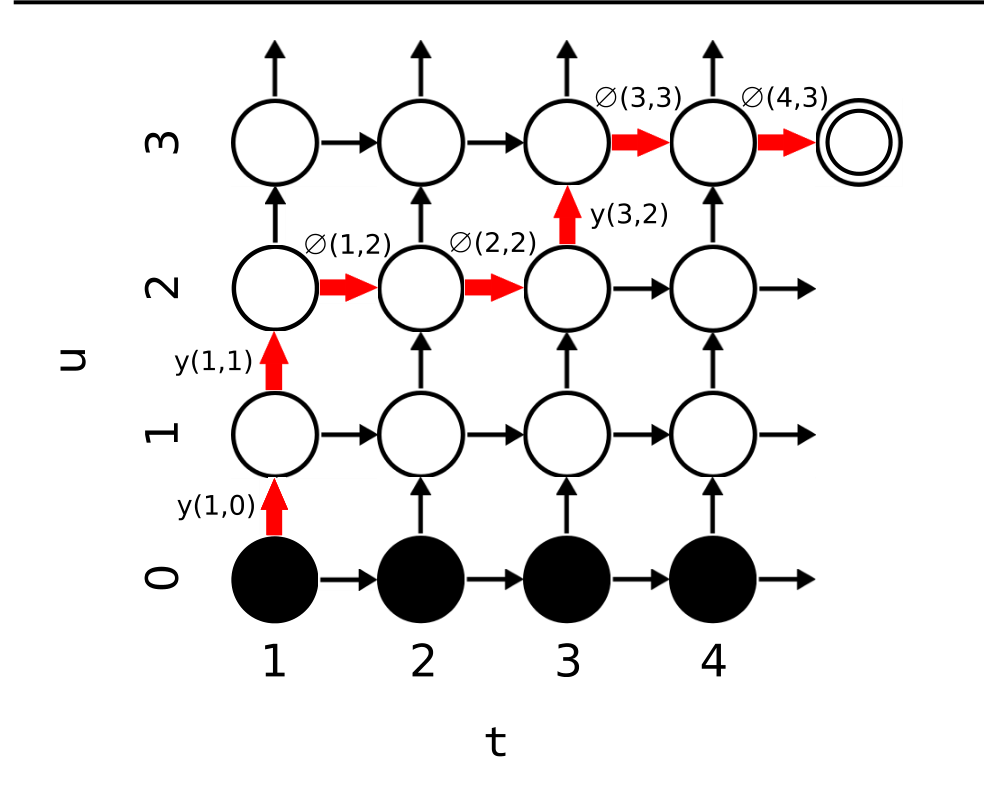
\includegraphics[width=0.58\linewidth]{report_figures/papers/figures/rnnt_alignment_lattice.png}
    \caption[Lưới xác suất biểu diễn các phép căn chỉnh trong RNN-T]{Lưới xác suất biểu diễn các phép căn chỉnh trong RNN-T \protect\cite{rnnt}.}
    \label{fig:rnnt-alignment-lattice}
\end{figure}

Trong huấn luyện, hàm mất mát RNN-T là log âm của xác suất chuỗi tham chiếu:

\begin{equation}
    \mathcal{L}_{\mathrm{RNNT}}
    =
    -\log P(Y\mid X).
\end{equation}

Xác suất tổng trên các đường căn chỉnh được tính hiệu quả bằng thuật toán forward--backward thay vì liệt kê từng đường đi \cite{rnnt}. Khi suy luận, mô hình có thể sử dụng greedy search hoặc beam search để tìm chuỗi token có xác suất cao. Vì quyết định đầu ra tại thời điểm hiện tại chỉ cần biểu diễn âm học đã có và lịch sử token, RNN-T phù hợp với nhận dạng theo luồng. Tuy nhiên, khả năng streaming thực tế còn phụ thuộc vào việc encoder có sử dụng ngữ cảnh tương lai hay toàn bộ câu nói.

\subsection{Conformer và Zipformer}

Encoder của hệ thống nhận dạng cần mô hình hóa cả quan hệ cục bộ, chẳng hạn sự biến đổi phổ trong các khung âm thanh lân cận, và quan hệ dài hạn giữa các phần cách xa nhau trong câu nói. Conformer kết hợp hai cơ chế tương ứng là convolution và multi-head self-attention \cite{conformer}. Một Conformer block có hai mô-đun feed-forward kiểu Macaron bao quanh mô-đun self-attention và mô-đun convolution. Self-attention khai thác tương tác toàn cục phụ thuộc nội dung, còn depthwise convolution một chiều khai thác các mẫu cục bộ theo thời gian. Kết quả thực nghiệm của công trình Conformer cho thấy mô-đun convolution là thành phần quan trọng đối với hiệu quả nhận dạng, trong khi cách bố trí hai feed-forward module với kết nối dư nửa bước cũng cải thiện chất lượng so với Transformer block thông thường \cite{conformer}.

Kiến trúc encoder trong Hình~\ref{fig:conformer-encoder} trước hết giảm tần suất khung bằng convolution subsampling, sau đó đưa biểu diễn qua nhiều Conformer block. Trong mỗi block, hai mô-đun feed-forward sử dụng kết nối dư với hệ số \(1/2\), còn self-attention và convolution lần lượt xử lý quan hệ toàn cục và cục bộ. Layer normalization được áp dụng sau chuỗi mô-đun để tạo đầu ra của block.

\begin{figure}[H]
    \centering
    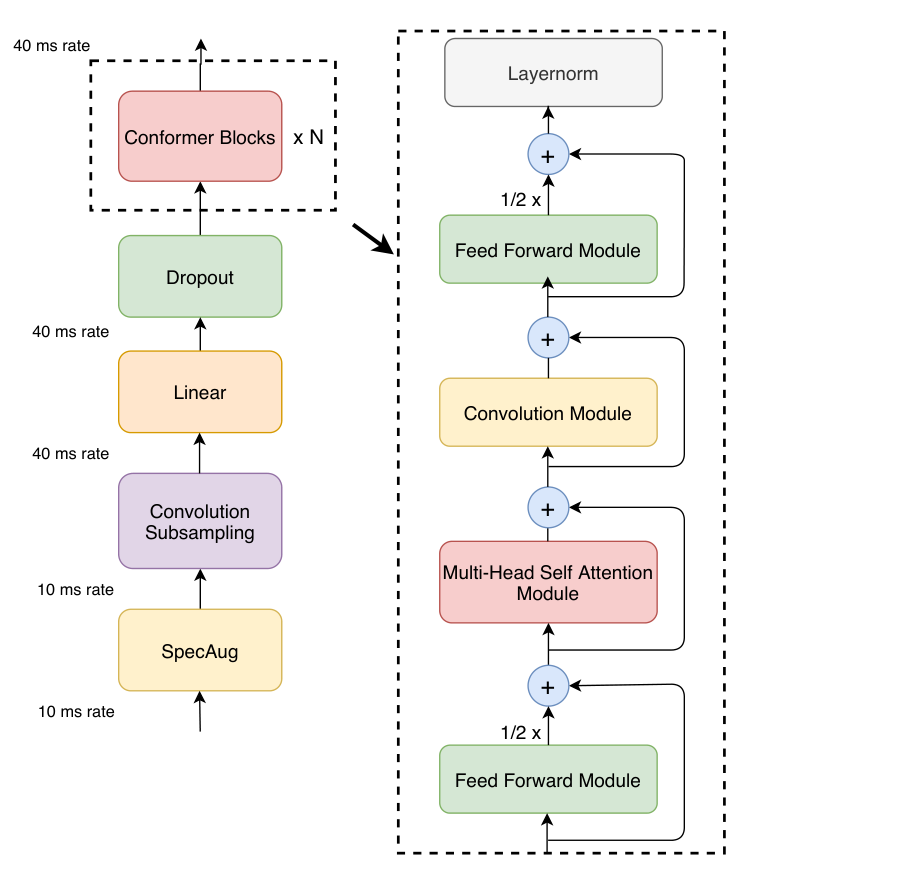
\includegraphics[width=\linewidth]{report_figures/papers/figures/conformer_encoder_cropped.png}
    \caption[Kiến trúc encoder và cấu trúc Conformer block]{Kiến trúc encoder và cấu trúc Conformer block \protect\cite{conformer}.}
    \label{fig:conformer-encoder}
\end{figure}

Hạn chế của self-attention là chi phí tính toán và bộ nhớ tăng theo bình phương độ dài chuỗi. Với tín hiệu tiếng nói có nhiều khung thời gian, việc duy trì cùng một tần suất khung ở tất cả các tầng làm tăng chi phí không cần thiết. Zipformer được đề xuất như một encoder nhanh hơn và tiết kiệm bộ nhớ hơn Conformer, đồng thời vẫn giữ khả năng mô hình hóa quan hệ cục bộ và toàn cục \cite{zipformer}.

Thay đổi quan trọng đầu tiên của Zipformer là cấu trúc encoder tương tự U-Net. Sau bước Conv-Embed, các stack encoder ở giữa hoạt động trên chuỗi đã được giảm tần suất khung; về cuối mạng, đặc trưng được tăng mẫu và kết hợp với các biểu diễn ở độ phân giải cao hơn. Theo cấu hình được trình bày trong công trình gốc, các stack lần lượt xử lý đặc trưng ở tần suất 50 Hz, 25 Hz, 12,5 Hz, 6,25 Hz, 12,5 Hz và 25 Hz \cite{zipformer}. Vì các tầng sâu nhất làm việc trên chuỗi ngắn hơn, chi phí của attention giảm đáng kể, trong khi các kết nối giữa nhiều độ phân giải giúp khôi phục thông tin thời gian cần thiết cho nhận dạng.

Thay đổi thứ hai nằm trong cấu trúc Zipformer block. Trọng số attention được tính một lần và tái sử dụng cho nhiều mô-đun, gồm hai mô-đun self-attention và một mô-đun non-linear attention. Việc dùng chung trọng số attention làm giảm các phép tính lặp lại nhưng vẫn cho phép block xử lý thông tin toàn cục qua nhiều phép biến đổi. Các kết nối bypass có hệ số học được điều chỉnh mức đóng góp giữa đầu vào và đầu ra của từng nhóm mô-đun \cite{zipformer}.

Zipformer còn thay LayerNorm bằng BiasNorm. Trong khi LayerNorm loại bỏ cả trung bình và độ lớn của vector, BiasNorm chỉ dịch chuyển vector bằng một độ lệch học được trước khi chuẩn hóa, nhờ đó encoder có thể giữ lại một phần thông tin liên quan đến độ lớn. Hai hàm kích hoạt SwooshR và SwooshL được thiết kế với hình dạng khác nhau cho các vị trí trong mô-đun feed-forward và convolution. Các thay đổi về chuẩn hóa và kích hoạt này là thành phần của kiến trúc Zipformer; ScaledAdam và lịch Eden được công trình đề xuất cho giai đoạn huấn luyện nhưng không làm thay đổi luồng suy luận của checkpoint đã huấn luyện \cite{zipformer}.

Hình~\ref{fig:zipformer-architecture} thể hiện kiến trúc tổng thể của Zipformer. Chuỗi đặc trưng được giảm mẫu dần từ 50 Hz xuống 6,25 Hz ở các stack giữa, sau đó tăng mẫu trở lại trước khi tạo đầu ra 25 Hz. Cách tổ chức nhiều độ phân giải này giúp encoder xử lý sâu hơn trên chuỗi ngắn ở tầng giữa, đồng thời vẫn giữ được thông tin thời gian cần thiết nhờ các bước tăng mẫu và kết nối giữa các mức tần suất khung.

\begin{figure}[H]
    \centering
    \makebox[\textwidth][c]{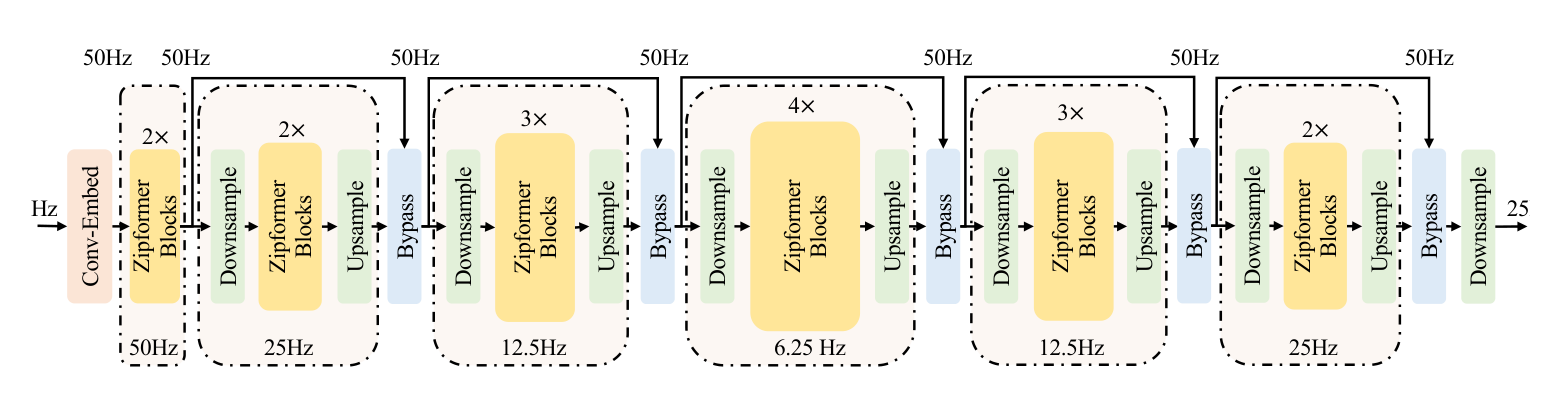
\includegraphics[width=1.12\textwidth]{report_figures/papers/figures/zipformer_overall_architecture_fig1.png}}
    \caption[Kiến trúc tổng thể của Zipformer]{Kiến trúc tổng thể của Zipformer \protect\cite{zipformer}.}
    \label{fig:zipformer-architecture}
\end{figure}

Trong mô hình nhận dạng hoàn chỉnh, Zipformer đóng vai trò encoder âm học của RNN-T. Encoder tạo biểu diễn từ chuỗi đặc trưng tiếng nói; prediction network mã hóa tiền tố token; joiner kết hợp hai biểu diễn để dự đoán token hoặc ký hiệu rỗng. Vì vậy, tên gọi Zipformer--RNN-T mô tả hai cấp khác nhau: Zipformer là kiến trúc encoder, còn RNN-T xác định cơ chế căn chỉnh, hàm mất mát và giải mã chuỗi.

Đồ án sử dụng checkpoint hynt/Zipformer-30M-RNNT-6000h cho tiếng Việt. Theo model card, checkpoint có khoảng 30 triệu tham số, sử dụng Zipformer với RNN-T loss và được huấn luyện trên khoảng 6000 giờ tiếng nói tiếng Việt được tập hợp từ nhiều bộ dữ liệu công khai \cite{zipformer6000h}. Mô hình được cung cấp ở định dạng phù hợp với Sherpa-ONNX và được triển khai cục bộ trong mô-đun ASR. Model card mô tả mô hình theo hướng tối ưu cho suy luận CPU tốc độ cao; tuy nhiên, hiệu năng sử dụng trong đồ án được xác định bằng thực nghiệm riêng trên môi trường triển khai thay vì sử dụng trực tiếp số liệu công bố của tác giả.


\section{Retrieval-Augmented Generation}

Retrieval-Augmented Generation (RAG) là hướng tiếp cận kết hợp một mô hình sinh với kho tri thức bên ngoài \cite{rag}. Trong hệ thống hỏi đáp thông thường, câu hỏi có thể được đưa trực tiếp vào mô hình ngôn ngữ lớn để sinh câu trả lời. Cách làm này thuận tiện nhưng có hạn chế: tri thức của mô hình được lưu gián tiếp trong tham số, có thể không cập nhật, khó kiểm soát nguồn và có nguy cơ tạo ra câu trả lời trôi chảy nhưng thiếu căn cứ. RAG thay đổi luồng xử lý bằng cách truy xuất tài liệu liên quan trước, đưa tài liệu đó vào ngữ cảnh đầu vào, rồi mới yêu cầu mô hình sinh câu trả lời.

Về mặt chức năng, một pipeline RAG gồm ba pha liên tiếp: Retrieval, Augmentation và Generation. Retrieval có nhiệm vụ tìm các đoạn tài liệu có liên quan đến câu hỏi. Augmentation xây dựng đầu vào cho mô hình sinh bằng cách ghép câu hỏi với các tài liệu truy xuất, chỉ dẫn hệ thống và các thông tin ngữ cảnh khác. Generation sử dụng mô hình ngôn ngữ lớn để tạo câu trả lời dựa trên phần ngữ cảnh đã được cung cấp.
\subsection{Retrieval: truy xuất tài liệu}

Pha Retrieval quyết định thông tin nào được đưa vào đầu vào của mô hình sinh. Nếu tài liệu truy xuất không chứa nội dung cần thiết, mô hình ngôn ngữ khó có thể tạo câu trả lời đúng dù khả năng sinh văn bản tốt. Ngược lại, nếu truy xuất đưa vào quá nhiều nội dung nhiễu, mô hình có thể bị phân tán hoặc sử dụng nhầm thông tin. Vì vậy, Retrieval không chỉ là bước tìm kiếm văn bản mà còn là bước chọn lọc tri thức cho toàn bộ pipeline.

Trong hệ thống hội thoại, câu hỏi đầu vào thường ngắn, chứa từ đệm, cách gọi phổ thông hoặc lỗi do nhận dạng tiếng nói. Chuẩn hóa truy vấn đưa các cách diễn đạt khác nhau về dạng nhất quán hơn trước khi tìm kiếm. Ví dụ, các cách gọi phổ thông có thể được ánh xạ về thuật ngữ thường gặp trong tài liệu dinh dưỡng. Mở rộng truy vấn bổ sung từ đồng nghĩa, thuật ngữ liên quan hoặc biến thể biểu đạt nhằm tăng khả năng khớp với tài liệu. Tuy nhiên, mở rộng truy vấn cũng có rủi ro: nếu bổ sung từ khóa không đúng ý định, truy vấn có thể bị lệch khỏi câu hỏi ban đầu và làm tăng nhiễu trong kết quả.

Một hướng mở rộng truy vấn khác là Hypothetical Document Embeddings (HyDE). Thay vì chỉ dùng câu hỏi ngắn, HyDE dùng mô hình ngôn ngữ để sinh một đoạn văn giả định có khả năng trả lời câu hỏi, sau đó mã hóa đoạn giả định này để truy xuất tài liệu thật \cite{hyde}. Ý tưởng chính là đoạn văn giả định thường giàu ngữ cảnh hơn câu hỏi ban đầu, từ đó có thể tạo embedding gần hơn với các tài liệu liên quan. Điểm đánh đổi là phương pháp này cần thêm một lượt sinh văn bản trước khi truy xuất, nên làm tăng độ trễ và cần được cân nhắc trong hệ thống tương tác bằng tiếng nói.

Với truy xuất ngữ nghĩa, tài liệu và truy vấn được ánh xạ vào một không gian vector liên tục. Bi-encoder mã hóa truy vấn và tài liệu độc lập, nhờ đó vector tài liệu có thể được tính trước và lưu trong kho dữ liệu \cite{sbert}. Khi có câu hỏi mới, hệ thống chỉ cần mã hóa câu hỏi và tìm các vector tài liệu gần nhất. Độ gần giữa truy vấn và tài liệu thường được đo bằng cosine similarity:

\begin{equation}
    \mathrm{sim}(q,d)
    =
    \frac{q \cdot d}{\lVert q\rVert\lVert d\rVert},
\end{equation}

trong đó \(q\) và \(d\) lần lượt là vector của truy vấn và tài liệu. Giá trị càng lớn cho thấy hai vector có hướng càng gần nhau trong không gian embedding. Cách truy xuất này phù hợp với câu hỏi tự nhiên vì có thể tìm các tài liệu gần nghĩa ngay cả khi chúng không chứa chính xác cùng từ khóa với truy vấn.

Khi số lượng vector lớn, việc so sánh truy vấn với toàn bộ kho dữ liệu có chi phí cao. Vector database giải quyết vấn đề này bằng cách lưu vector cùng metadata và cung cấp cơ chế tìm kiếm láng giềng gần nhất xấp xỉ. Một cấu trúc phổ biến là Hierarchical Navigable Small World (HNSW), tổ chức vector thành đồ thị nhiều tầng để tìm kiếm nhanh hơn so với duyệt tuyến tính \cite{hnsw}. Tìm kiếm bắt đầu ở tầng thưa để tiếp cận nhanh vùng gần truy vấn, sau đó đi xuống các tầng dày hơn để tinh chỉnh kết quả. Trong hệ thống ứng dụng, HNSW thường được vector database triển khai sẵn; người phát triển sử dụng giao diện truy vấn thay vì tự hiện thực thuật toán đồ thị.

Bi-encoder có tốc độ cao nhưng truy vấn và tài liệu được mã hóa độc lập, nên mô hình không quan sát trực tiếp tương tác giữa từng token của hai văn bản. Vì vậy, nhiều hệ thống RAG sử dụng truy xuất hai bước. Bước đầu dùng bi-encoder để lấy một tập ứng viên đủ rộng. Bước sau dùng cross-encoder để đánh giá lại từng cặp truy vấn--tài liệu. Cross-encoder đưa đồng thời câu hỏi và tài liệu vào cùng một mô hình, nhờ đó khai thác được tương tác token giữa hai văn bản và thường cho điểm liên quan chính xác hơn. Đổi lại, cross-encoder phải chạy suy luận riêng cho từng cặp, nên chỉ phù hợp với tập ứng viên đã được thu hẹp.

\subsection{Augmentation: xây dựng ngữ cảnh cho mô hình sinh}

Sau khi có các tài liệu liên quan, pha Augmentation quyết định cách đưa tri thức vào đầu vào của LLM. Đây là bước nối giữa truy xuất và sinh câu trả lời. Đầu vào của mô hình không chỉ gồm câu hỏi hiện tại, mà còn có thể bao gồm chỉ dẫn hệ thống, các đoạn văn bản truy xuất, lịch sử hội thoại, bản tóm tắt phiên và yêu cầu về phong cách trả lời. Việc tổ chức các thành phần này ảnh hưởng trực tiếp đến khả năng mô hình sử dụng đúng tài liệu.

Một prompt RAG cần làm rõ ba điểm: mô hình phải trả lời trong phạm vi nào, nguồn thông tin nào được phép sử dụng và phải làm gì khi tài liệu không đủ hỗ trợ kết luận. Với chủ đề có liên quan đến sức khỏe như dinh dưỡng, chỉ dẫn hệ thống cần giới hạn vai trò của mô hình ở mức cung cấp thông tin tham khảo, tránh chẩn đoán, kê đơn hoặc đưa ra chỉ định điều trị. Các đoạn tài liệu truy xuất nên được đặt ở vị trí rõ ràng trong prompt để mô hình phân biệt ngữ cảnh nguồn với câu hỏi của người dùng.

Pha Augmentation cũng phải xử lý giới hạn độ dài ngữ cảnh. Nếu đưa quá ít tài liệu, mô hình có thể thiếu bằng chứng để trả lời. Nếu đưa quá nhiều tài liệu, prompt dài hơn, chi phí suy luận tăng và nội dung nhiễu có thể làm câu trả lời kém tập trung. Do đó, số lượng đoạn văn bản đưa vào prompt là một tham số quan trọng của hệ thống RAG. Trong pipeline hai bước, reranker có vai trò chọn một tập nhỏ hơn từ các ứng viên ban đầu để cân bằng giữa độ phủ thông tin và mức nhiễu trong prompt.

Trong hội thoại nhiều lượt, Augmentation còn cần xử lý ngữ cảnh phiên. Câu hỏi hiện tại có thể phụ thuộc vào lượt trước, ví dụ người dùng hỏi tiếp bằng các đại từ hoặc cụm như ``vậy tôi nên ăn gì''. Nếu bỏ qua lịch sử, hệ thống có thể không hiểu đối tượng mà câu hỏi đang nhắc tới. Tuy nhiên, đưa toàn bộ lịch sử vào prompt làm độ dài tăng dần theo thời gian. Vì vậy, hệ thống thường giữ một số lượt gần nhất và bổ sung bản tóm tắt ngắn của các lượt cũ hơn. Cách làm này giúp duy trì ngữ cảnh hội thoại mà vẫn kiểm soát kích thước đầu vào của LLM.

\subsection{Generation: sinh câu trả lời bằng mô hình ngôn ngữ lớn}

Pha Generation sử dụng mô hình ngôn ngữ lớn để tạo câu trả lời từ prompt đã được xây dựng ở pha Augmentation. Đây là nơi LLM tham gia trực tiếp vào RAG. Nhiệm vụ của LLM không phải là tự trả lời hoàn toàn từ tri thức tham số, mà là đọc câu hỏi, đọc các đoạn ngữ cảnh được truy xuất và diễn đạt câu trả lời phù hợp với chỉ dẫn hệ thống.

Phần lớn LLM hiện đại dựa trên kiến trúc Transformer \cite{transformer}. Thành phần cốt lõi của Transformer là self-attention, cho phép mô hình xác định mức liên quan giữa các token trong cùng một chuỗi. Với truy vấn \(Q\), khóa \(K\) và giá trị \(V\), scaled dot-product attention được xác định bởi:

\begin{equation}
    \mathrm{Attention}(Q,K,V)
    =
    \mathrm{softmax}\left(
    \frac{QK^{T}}{\sqrt{d_k}}
    \right)V.
\end{equation}

Cơ chế này giúp mô hình kết hợp thông tin từ nhiều vị trí trong prompt, bao gồm câu hỏi, chỉ dẫn và tài liệu truy xuất. Khi sinh câu trả lời, mô hình thường hoạt động theo cơ chế tự hồi quy: token tiếp theo được dự đoán dựa trên toàn bộ chuỗi token đã có trước đó. Xác suất của một chuỗi đầu ra có thể viết dưới dạng:

\begin{equation}
    P(y_1,\ldots,y_n \mid c)
    =
    \prod_{i=1}^{n}P(y_i \mid y_1,\ldots,y_{i-1},c),
\end{equation}

trong đó \(c\) là ngữ cảnh đầu vào gồm câu hỏi, tài liệu truy xuất và các chỉ dẫn liên quan. Công thức này cho thấy chất lượng câu trả lời phụ thuộc đồng thời vào năng lực sinh của mô hình và chất lượng ngữ cảnh được cung cấp. Nếu ngữ cảnh thiếu hoặc sai, mô hình vẫn có thể sinh câu trả lời trôi chảy nhưng không đáng tin cậy. Ngược lại, nếu ngữ cảnh tốt nhưng prompt không ràng buộc rõ, mô hình có thể không sử dụng hết thông tin truy xuất hoặc suy diễn vượt quá tài liệu.

Trong RAG, một yêu cầu quan trọng đối với pha Generation là tính bám ngữ cảnh. Câu trả lời cần được hỗ trợ bởi các đoạn văn bản đã truy xuất, tránh thêm khuyến nghị không có trong nguồn. Với hệ thống tư vấn dinh dưỡng, điều này đặc biệt quan trọng vì câu trả lời có thể ảnh hưởng đến lựa chọn ăn uống của người dùng. Khi tài liệu không đủ thông tin, mô hình nên trả lời thận trọng hoặc yêu cầu người dùng cung cấp thêm chi tiết thay vì cố gắng đưa ra kết luận chắc chắn.

Mô hình sinh câu trả lời được sử dụng trong đồ án là Qwen-3-4b-2507, tương ứng với model card chính thức Qwen3-4B-Instruct-2507. Đây là mô hình ngôn ngữ nhân quả thuộc họ Qwen3, được phát triển cho chế độ non-thinking và đã qua giai đoạn hậu huấn luyện để tuân theo chỉ dẫn \cite{qwen3,qwen3modelcard}. Khác với các biến thể có cơ chế suy luận dài, phiên bản Instruct-2507 chỉ sinh câu trả lời cuối cùng mà không tạo các khối suy nghĩ trung gian. Đặc điểm này phù hợp với hệ thống hội thoại bằng tiếng nói, nơi câu trả lời cần ngắn gọn, trực tiếp và có độ trễ thấp.

Theo model card, Qwen3-4B-Instruct-2507 có khoảng 4,0 tỉ tham số, trong đó 3,6 tỉ tham số không thuộc embedding; mô hình gồm 36 lớp Transformer và sử dụng Grouped-Query Attention với 32 attention head cho truy vấn và 8 head cho khóa--giá trị \cite{qwen3modelcard}. Grouped-Query Attention giúp giảm chi phí lưu trữ và truy cập key-value cache trong quá trình suy luận so với việc dùng cùng số lượng head cho \(Q\), \(K\) và \(V\), trong khi vẫn giữ khả năng biểu diễn của nhiều head truy vấn. Mô hình hỗ trợ ngữ cảnh dài tới 262144 token, nhưng trong hệ thống RAG của đồ án, ngữ cảnh thực tế được giới hạn bởi số đoạn truy xuất, lịch sử hội thoại và yêu cầu độ trễ.

\begin{table}[H]
    \centering
    \begin{tabular}{p{5.2cm}p{8.5cm}}
        \toprule
        Thuộc tính      & Giá trị                                                          \\
        \midrule
        Loại mô hình    & Causal language model, hậu huấn luyện cho chỉ dẫn                \\
        Số tham số      & Khoảng 4,0 tỉ tham số; 3,6 tỉ tham số không tính embedding       \\
        Số lớp          & 36 lớp Transformer                                               \\
        Attention       & Grouped-Query Attention, 32 head cho \(Q\) và 8 head cho \(K,V\) \\
        Độ dài ngữ cảnh & 262144 token theo model card                                     \\
        Chế độ suy luận & Non-thinking mode, không sinh khối suy nghĩ trung gian           \\
        Giấy phép       & Apache 2.0                                                       \\
        \bottomrule
    \end{tabular}
    \caption[Một số thông số của Qwen3-4B-Instruct-2507]{Một số thông số của Qwen3-4B-Instruct-2507 theo model card chính thức \cite{qwen3modelcard}.}
    \label{tab:qwen3-4b-specs}
\end{table}

Bảng~\ref{tab:qwen3-4b-specs} cho thấy mô hình được lựa chọn vì cân bằng giữa kích thước và khả năng triển khai. So với các mô hình lớn hơn trong cùng họ, bản 4B có chi phí bộ nhớ và thời gian suy luận thấp hơn, phù hợp hơn với yêu cầu demo và thử nghiệm cục bộ. Trong hệ thống, Qwen-3-4b-2507 không được xem là nguồn tri thức chính mà đảm nhiệm pha Generation: tổng hợp câu trả lời từ câu hỏi, lịch sử hội thoại và các đoạn văn bản đã truy xuất. Chất lượng câu trả lời vì vậy phụ thuộc đồng thời vào khả năng tuân theo chỉ dẫn của mô hình, chất lượng các đoạn ngữ cảnh được cung cấp và cách prompt ràng buộc mô hình chỉ trả lời trong phạm vi tài liệu.

\section{Tổng hợp tiếng nói}

Tổng hợp tiếng nói là bài toán chuyển văn bản thành tín hiệu âm thanh sao cho nội dung được đọc đúng, phát âm rõ, nhịp ngắt tự nhiên và có thể nghe được trong ngữ cảnh hội thoại. Trong hệ thống tư vấn dinh dưỡng qua kênh tiếng nói, TTS không chỉ là mô-đun ở cuối pipeline mà còn ảnh hưởng trực tiếp tới cảm nhận thời gian thực của người dùng. Một câu trả lời có nội dung đúng nhưng bắt đầu phát quá muộn, ngắt nghỉ thiếu tự nhiên hoặc phát âm sai thuật ngữ dinh dưỡng đều làm giảm chất lượng tương tác.

Đối với tiếng Việt, bài toán TTS có một số yêu cầu riêng. Thanh điệu là một phần của âm tiết và có thể làm thay đổi nghĩa của từ, do đó lỗi dấu hoặc lỗi trường độ dễ làm người nghe hiểu sai. Ngoài ra, câu trả lời trong chủ đề dinh dưỡng thường chứa số, đơn vị đo, tên vi chất, tên bệnh lý phổ biến và từ vay mượn. Những yếu tố này khiến khâu chuẩn hóa văn bản, biểu diễn phát âm và chia đoạn đầu vào trở nên quan trọng trước khi sinh âm thanh.

\subsection{Chuẩn hóa văn bản và biểu diễn phát âm}

Văn bản đầu vào của TTS thường không ở dạng có thể đọc trực tiếp. Các biểu diễn như ``100 mg'', ``vitamin D3'', ``omega-3'', tỉ lệ phần trăm, số thập phân hoặc ký hiệu y học cần được chuyển về dạng phát âm phù hợp. Chuẩn hóa văn bản vì vậy có nhiệm vụ biến chuỗi ký tự thành chuỗi từ có thể đọc tự nhiên, đồng thời loại bỏ hoặc thay thế các ký hiệu không nên phát âm nguyên dạng.

Sau chuẩn hóa, hệ thống có thể ánh xạ văn bản sang biểu diễn phát âm. Với tiếng Việt, biểu diễn này cần bảo toàn âm đầu, âm chính, âm cuối và thanh điệu. Các từ nước ngoài, tên riêng hoặc cách viết tắt không phải lúc nào cũng tuân theo quy tắc chữ--âm thông thường, nên phần mềm TTS thường kết hợp bộ chuyển đổi chữ sang âm với từ điển phát âm. Cách biểu diễn theo phát âm giúp mô hình nhận đầu vào gần với cách đọc hơn so với chuỗi chữ viết ban đầu.

\subsection{Neural audio codec}

Các hệ thống TTS hiện đại không nhất thiết sinh trực tiếp từng mẫu waveform. Một hướng phổ biến là dùng neural audio codec để nén âm thanh thành chuỗi mã rời rạc rồi tái tạo waveform từ chuỗi mã đó. Gọi \(x\) là tín hiệu âm thanh, \(E_{\mathrm{codec}}\) là bộ mã hóa và \(D_{\mathrm{codec}}\) là bộ giải mã, quá trình này có thể viết:

\begin{equation}
    z = E_{\mathrm{codec}}(x),
    \qquad
    \hat{x} = D_{\mathrm{codec}}(z),
\end{equation}

trong đó \(z = (z_1,\ldots,z_M)\) là chuỗi token âm thanh rời rạc và \(\hat{x}\) là waveform được khôi phục. So với việc mô hình hóa trực tiếp waveform, chuỗi token codec ngắn hơn và có cấu trúc gần với bài toán sinh chuỗi. Nhờ vậy, một mô hình ngôn ngữ có thể được dùng để sinh token tiếng nói, còn codec decoder đảm nhiệm việc chuyển token thành tín hiệu âm thanh.

Chất lượng của codec ảnh hưởng trực tiếp tới chất lượng TTS. Nếu codec nén quá mạnh, âm thanh sau giải mã có thể mất chi tiết về âm sắc, độ rõ hoặc ngữ điệu. Nếu chuỗi token quá dài, mô hình sinh token phải xử lý nhiều bước hơn, làm tăng độ trễ. Vì vậy, neural audio codec đóng vai trò cân bằng giữa chất lượng tái tạo, tốc độ giải mã và chi phí sinh tự hồi quy.

\subsection{Mô hình ngôn ngữ sinh token tiếng nói}

Trong hướng neural codec language model, TTS được chuyển thành bài toán sinh chuỗi token âm thanh có điều kiện theo văn bản \cite{valle}. Thay vì dự đoán mẫu âm thanh liên tục, mô hình học phân phối:

\begin{equation}
    P(z_1,\ldots,z_M \mid c)
    =
    \prod_{i=1}^{M}
    P(z_i \mid z_1,\ldots,z_{i-1},c),
\end{equation}

trong đó \(c\) là điều kiện đầu vào, bao gồm biểu diễn văn bản và có thể kèm thông tin người nói tham chiếu; \(z_i\) là token tiếng nói tại bước \(i\). Sau khi mô hình sinh xong một phần hoặc toàn bộ chuỗi token, neural codec decoder chuyển các token này thành waveform.

Điều kiện người nói tham chiếu thường gồm hai phần: văn bản tham chiếu và chuỗi token codec được trích ra từ một đoạn âm thanh mẫu. Văn bản tham chiếu giúp mô hình biết nội dung tương ứng với chuỗi token mẫu, còn token codec mang thông tin về âm sắc và cách phát âm của người nói. Nhờ cơ chế này, mô hình có thể tổng hợp cùng một nội dung theo các mẫu người nói khác nhau mà không cần huấn luyện lại toàn bộ hệ thống.

\subsection{Kiến trúc của VieNeu-TTS}

VieNeu-TTS là một mô hình TTS tiếng Việt hỗ trợ nhân bản tiếng nói tức thời từ một đoạn tham chiếu ngắn \cite{vieneutts}. Theo model card chính thức, phiên bản VieNeu-TTS-0.3B được huấn luyện từ đầu trên bộ dữ liệu tiếng Việt quy mô khoảng 1000 giờ và sử dụng backbone theo kiến trúc Qwen3ForCausalLM \cite{vieneutts03b}. Ở mức cơ sở lý thuyết, có thể xem VieNeu-TTS như một trường hợp ứng dụng của kiến trúc Transformer nhân quả cho bài toán sinh token tiếng nói tiếng Việt.

Backbone Qwen3ForCausalLM vẫn là một mô hình ngôn ngữ nhân quả dựa trên Transformer, nhưng trong VieNeu-TTS, miền sinh không phải token văn bản hội thoại mà là token tiếng nói. Về kiến trúc, mô hình gồm các lớp Transformer decoder xếp chồng, sử dụng cơ chế self-attention có mặt nạ nhân quả để tại mỗi bước chỉ quan sát các token điều kiện và các token đã sinh trước đó. Trạng thái ẩn cuối cùng được ánh xạ qua lớp dự đoán để tạo phân phối xác suất trên không gian token tiếng nói, sau đó mô hình chọn token tiếp theo theo cơ chế tự hồi quy. Cách tổ chức này phù hợp với TTS dựa trên codec vì chuỗi âm thanh đã được rời rạc hóa thành một bài toán sinh chuỗi.

Đầu vào của mô hình gồm văn bản cần đọc sau khi chuẩn hóa phát âm, văn bản tham chiếu và chuỗi token codec được trích từ tiếng nói tham chiếu. Văn bản tham chiếu giúp mô hình liên hệ chuỗi token mẫu với nội dung đã được đọc, còn token tham chiếu mang thông tin về âm sắc, nhịp nói và đặc trưng người nói. Từ các điều kiện đó, mô hình sinh tiếp chuỗi token tiếng nói cho văn bản đích.

\begin{figure}[H]
    \centering
    \resizebox{\textwidth}{!}{%
        \begin{tikzpicture}[
            font=\small,
            node distance=1.1cm and 1.3cm,
            block/.style={
                    draw,
                    rounded corners,
                    align=center,
                    minimum height=1.15cm,
                    text width=3.2cm,
                    fill=blue!6
                },
            model/.style={
                    draw,
                    rounded corners,
                    align=center,
                    minimum height=1.25cm,
                    text width=3.6cm,
                    fill=orange!12
                },
            codec/.style={
                    draw,
                    rounded corners,
                    align=center,
                    minimum height=1.15cm,
                    text width=3.2cm,
                    fill=green!10
                },
            arrow/.style={-{Latex[length=2.5mm]}, thick}
            ]
            \node[block] (target_text) {Văn bản cần đọc\\sau chuẩn hóa phát âm};
            \node[block, below=of target_text] (ref_text) {Văn bản tham chiếu};
            \node[block, below=of ref_text] (ref_audio) {Token tiếng nói\\tham chiếu};

            \node[model, right=2.0cm of ref_text] (backbone) {Backbone\\Qwen3ForCausalLM};
            \node[block, right=1.8cm of backbone] (speech_tokens) {Token tiếng nói\\được sinh};
            \node[codec, right=1.8cm of speech_tokens] (decoder) {Neural codec\\decoder};
            \node[block, right=1.8cm of decoder] (waveform) {Waveform\\tiếng nói đầu ra};

            \draw[arrow] (target_text.east) -- (backbone.west);
            \draw[arrow] (ref_text.east) -- (backbone.west);
            \draw[arrow] (ref_audio.east) -- (backbone.west);
            \draw[arrow] (backbone) -- node[above]{tự hồi quy} (speech_tokens);
            \draw[arrow] (speech_tokens) -- (decoder);
            \draw[arrow] (decoder) -- (waveform);
        \end{tikzpicture}%
    }
    \caption{Kiến trúc khái quát của VieNeu-TTS.}
    \label{fig:vieneutts-architecture}
\end{figure}

Sau khi chuỗi token tiếng nói được sinh ra, một neural codec decoder tái tạo waveform tương ứng. Như vậy, quá trình tổng hợp được tách thành hai mức: mô hình ngôn ngữ xử lý cấu trúc rời rạc của tiếng nói, còn codec decoder xử lý việc khôi phục tín hiệu âm thanh liên tục. Cách tách này giúp tận dụng khả năng sinh chuỗi của mô hình ngôn ngữ, đồng thời tránh phải dự đoán trực tiếp từng mẫu waveform.

Quá trình huấn luyện của mô hình có thể hiểu ở mức khái quát như sau. Từ các cặp âm thanh--văn bản trong bộ dữ liệu huấn luyện, codec trước hết biểu diễn âm thanh thành chuỗi token rời rạc. Văn bản được chuẩn hóa và ánh xạ sang biểu diễn phát âm. Backbone Qwen3ForCausalLM sau đó được huấn luyện theo kiểu mô hình ngôn ngữ nhân quả: với văn bản và token tiếng nói tham chiếu làm điều kiện, mô hình dự đoán token tiếng nói tiếp theo của đoạn cần tổng hợp. Hàm mục tiêu tương ứng là cực đại hóa xác suất của chuỗi token tiếng nói đúng, hay tương đương cực tiểu hóa cross-entropy trên token sinh ra. Cách huấn luyện này biến TTS thành bài toán dự đoán chuỗi rời rạc, tương tự sinh ngôn ngữ, nhưng miền token đầu ra là token âm thanh.

Đối với hệ thống hội thoại, một điểm quan trọng là khả năng phát âm thanh trước khi toàn bộ câu trả lời được tổng hợp xong. Với mô hình sinh token tiếng nói, streaming có thể được tổ chức bằng cách gom một số token mới thành cửa sổ giải mã. Mỗi cửa sổ có thể sử dụng thêm một phần ngữ cảnh quá khứ và một phần ngữ cảnh tương lai ngắn để giảm đứt gãy ở biên đoạn. Các đoạn waveform sau giải mã được nối bằng kỹ thuật overlap-add hoặc các biến thể tương tự để làm mượt ranh giới giữa các đoạn. Kích thước cửa sổ càng nhỏ thì âm thanh đầu tiên có thể xuất hiện sớm hơn, nhưng nguy cơ giảm độ liền mạch và tự nhiên cũng cao hơn.

\chapter{GIẢI PHÁP ĐỀ XUẤT}

\section{Kiến trúc hệ thống}

Chương này trình bày giải pháp ở mức thiết kế hệ thống và quy trình xử lý, chưa đi vào tên công cụ, framework hoặc checkpoint cụ thể. Các lựa chọn triển khai chi tiết sẽ được trình bày ở Chương 4. Ở mức giải pháp, hệ thống được tổ chức thành pipeline mô-đun gồm giao diện người dùng, mô-đun điều phối, mô-đun ASR, mô-đun xử lý hội thoại, LLM, database, bộ nhớ phiên và mô-đun TTS streaming.

Hình~\ref{fig:proposed-architecture-generic} trình bày kiến trúc hệ thống và luồng dữ liệu chính của giải pháp.

\begin{center}
    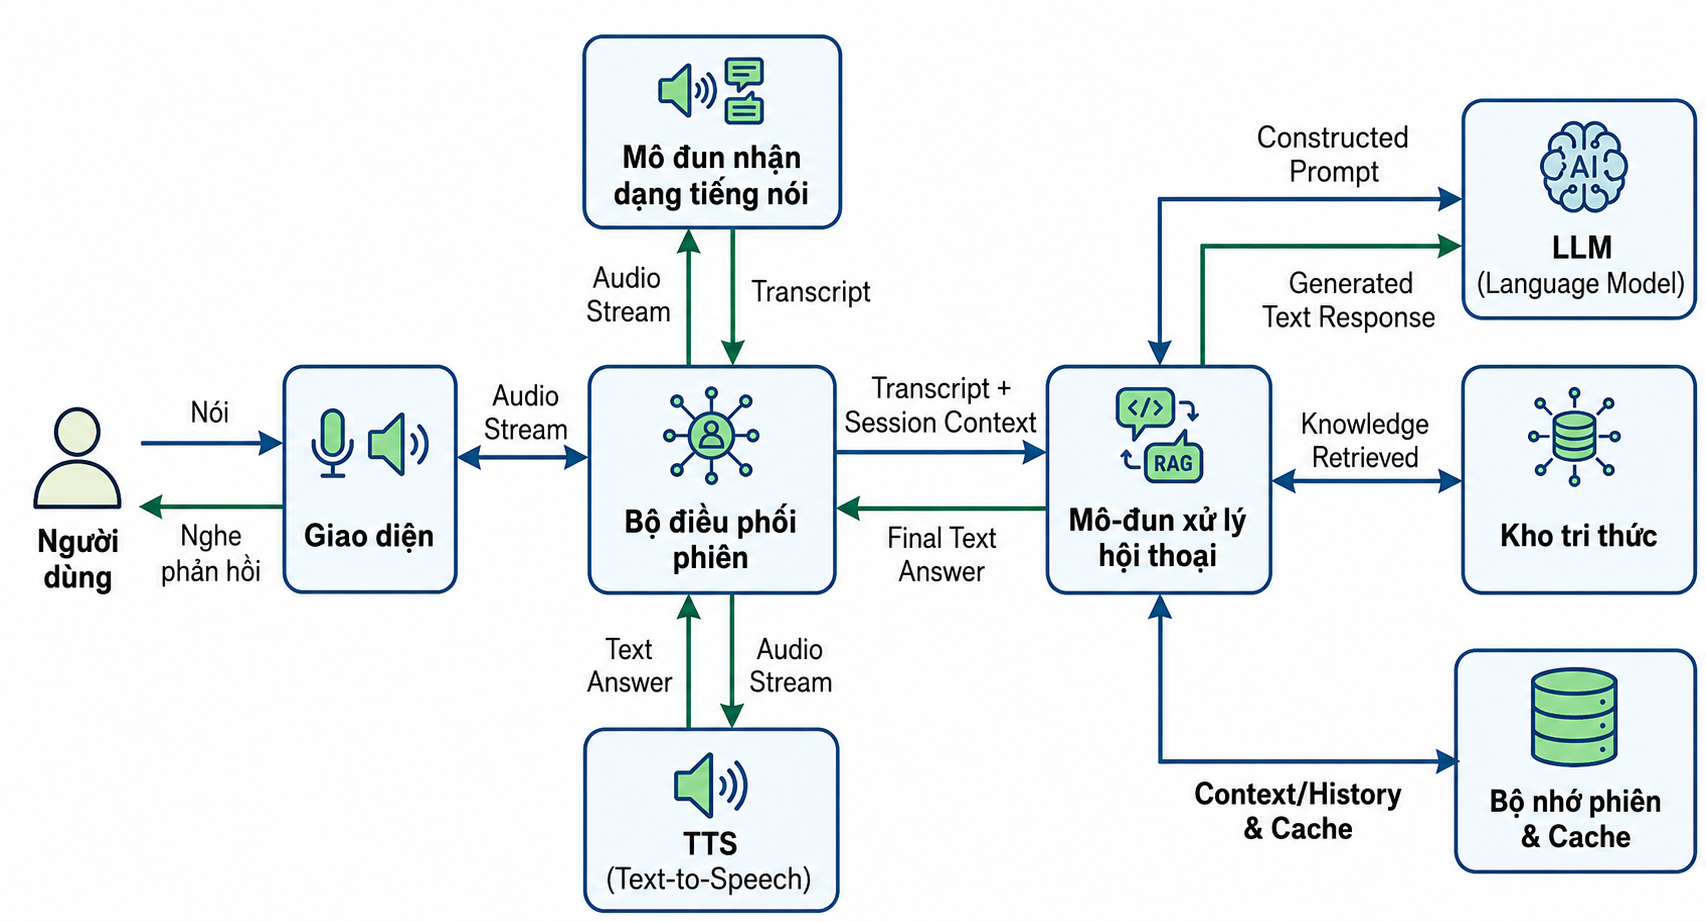
\includegraphics[width=\textwidth]{report_figures/chapter3_architecture_simplified.png}
    \captionof{figure}{Kiến trúc hệ thống và luồng dữ liệu của giải pháp}
    \label{fig:proposed-architecture-generic}
\end{center}
\nopagebreak[4]

Trong Hình~\ref{fig:proposed-architecture-generic}, hệ thống được chia thành ba nhóm xử lý chính. Nhóm thứ nhất là kênh tương tác với người dùng, gồm giao diện thu tiếng nói và phát âm thanh phản hồi. Giao diện không xử lý nội dung tư vấn mà chỉ chuẩn hóa âm thanh đầu vào, gửi các đoạn audio ngắn tới hệ thống và phát lại audio stream nhận được từ phía sau.

Nhóm thứ hai là bộ điều phối phiên. Thành phần này nằm giữa giao diện và các mô-đun xử lý, có nhiệm vụ giữ trạng thái của từng phiên hội thoại và định tuyến dữ liệu theo đúng thứ tự. Audio stream từ giao diện được chuyển tới mô-đun ASR; transcript cuối cùng từ ASR được ghép với lịch sử hội thoại và bản tóm tắt phiên trước khi gửi sang mô-đun xử lý hội thoại. Khi nhận text stream từ mô-đun xử lý hội thoại, bộ điều phối chia văn bản thành các đoạn phù hợp để gửi sang TTS, sau đó chuyển audio stream phản hồi về giao diện.

Nhóm thứ ba là các mô-đun AI và lưu trữ tri thức. Mô-đun ASR biến tín hiệu tiếng nói thành transcript. Mô-đun xử lý hội thoại kiểm tra phạm vi câu hỏi, chuẩn hóa truy vấn, truy xuất tri thức từ database, chọn lại các đoạn văn bản phù hợp và xây dựng đầu vào có ngữ cảnh cho LLM. LLM sinh câu trả lời theo luồng thay vì chờ hoàn thành toàn bộ văn bản. Mô-đun TTS streaming nhận từng đoạn văn bản và tổng hợp thành âm thanh để trả về người dùng sớm nhất có thể.

Database trong Hình~\ref{fig:proposed-architecture-generic} đại diện cho kho tri thức đã được mã hóa thành các vector phục vụ truy xuất ngữ nghĩa. Bộ nhớ phiên lưu lịch sử hội thoại, bản tóm tắt theo session và retrieval cache. Nhờ đó, hệ thống có thể duy trì ngữ cảnh giữa các lượt hỏi đáp, đồng thời tránh lặp lại một số bước truy xuất khi câu hỏi lặp lại hoặc gần nghĩa. Khi người dùng ngắt lời trong lúc hệ thống đang phát âm thanh, bộ điều phối gửi tín hiệu hủy để dừng phản hồi cũ và chuyển sang xử lý lượt nói mới.

Cách tổ chức này tách rõ trách nhiệm giữa các thành phần: giao diện phụ trách tương tác, bộ điều phối phụ trách luồng dữ liệu và trạng thái phiên, các mô-đun AI phụ trách nhận dạng--truy xuất--sinh--tổng hợp, còn database và bộ nhớ phiên phụ trách lưu trữ. Nhờ vậy, giải pháp có thể đo thời gian từng giai đoạn, thay thế từng mô-đun khi cần và phân tích rõ điểm gây độ trễ trong toàn bộ pipeline.

\begin{table}[H]
    \centering
    \begin{tabular}{|p{3.2cm}|p{10cm}|}
        \hline
        \textbf{Thành phần}    & \textbf{Vai trò}                                                                 \\
        \hline
        Giao diện              & Thu âm, gửi dữ liệu tiếng nói và phát âm thanh phản hồi cho người dùng.          \\
        \hline
        Mô-đun điều phối       & Điều phối audio stream, transcript, text stream, text segment và audio stream.   \\
        \hline
        Mô-đun ASR             & Chuyển tín hiệu tiếng nói tiếng Việt thành transcript.                           \\
        \hline
        Mô-đun xử lý hội thoại & Kiểm tra phạm vi, truy xuất tri thức, reranking và xây dựng đầu vào có ngữ cảnh. \\
        \hline
        LLM                    & Sinh câu trả lời dựa trên câu hỏi, lịch sử hội thoại và ngữ cảnh truy xuất.      \\
        \hline
        Mô-đun TTS streaming   & Chuyển các đoạn văn bản trả lời thành audio stream.                              \\
        \hline
        Database               & Lưu kho tri thức dạng vector và phục vụ truy xuất ngữ nghĩa.                     \\
        \hline
        Bộ nhớ phiên           & Lưu lịch sử, bản tóm tắt theo session và retrieval cache.                        \\
        \hline
    \end{tabular}
    \caption{Vai trò của các thành phần trong giải pháp}
    \label{tab:component-roles}
\end{table}

\subsection{Hai luồng xử lý chính}

Từ kiến trúc hệ thống ở Hình~\ref{fig:proposed-architecture-generic}, có thể tách hoạt động của voicebot thành hai luồng xử lý chính. Luồng thứ nhất là luồng hỏi đáp thông thường, mô tả đường đi của dữ liệu từ tiếng nói đầu vào tới âm thanh phản hồi. Luồng thứ hai là luồng barge-in, mô tả cách hệ thống hủy phản hồi cũ khi người dùng bắt đầu nói trong lúc bot đang phát âm thanh.

\begin{center}
    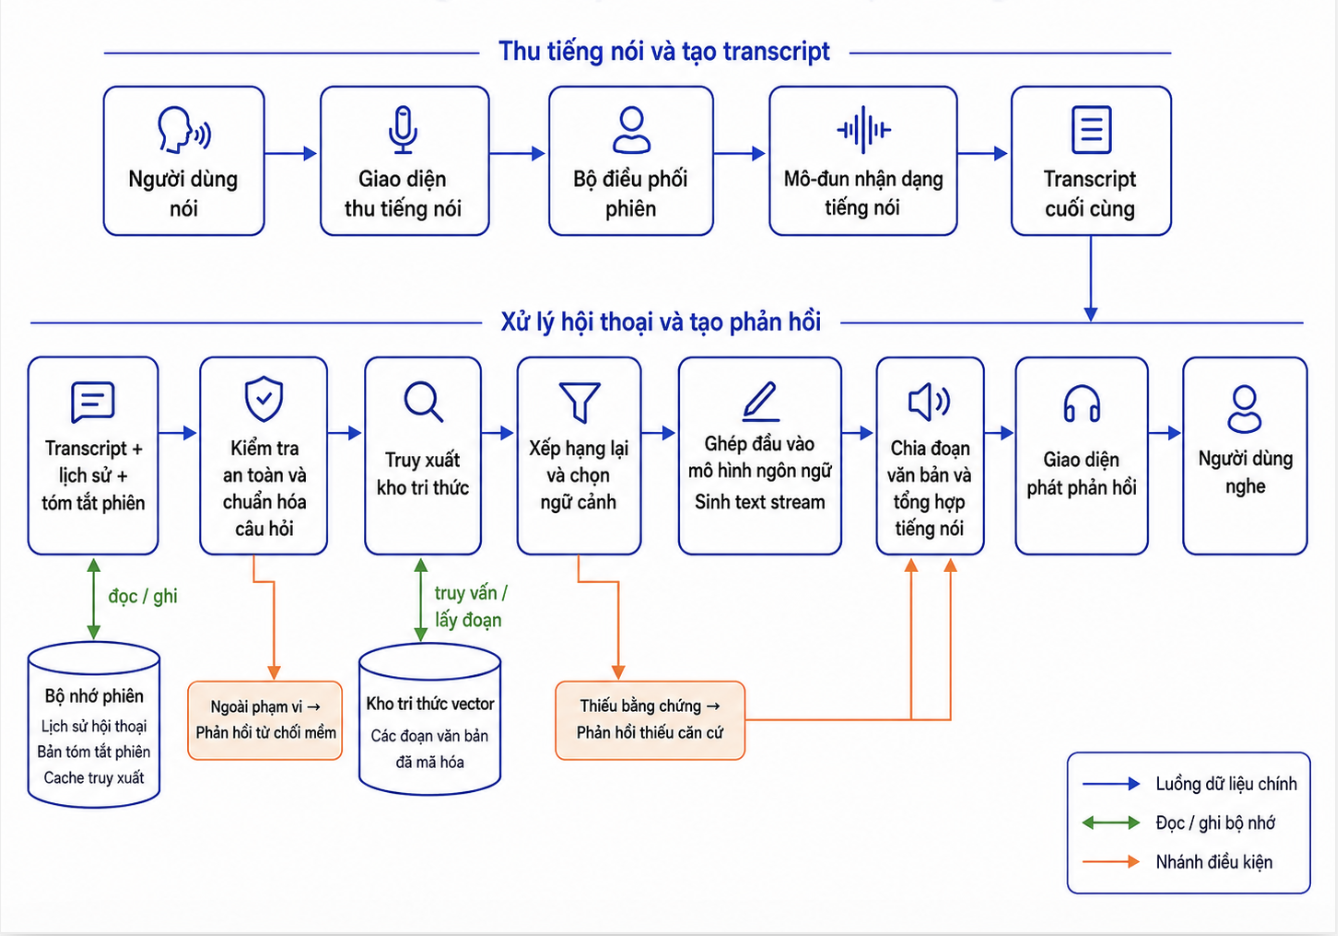
\includegraphics[width=\textwidth,height=0.72\textheight,keepaspectratio]{report_figures/main_qa_flow.png}
    \captionof{figure}{Luồng hỏi đáp chính của hệ thống}
    \label{fig:main-qa-flow}
\end{center}
\nopagebreak[4]

Hình~\ref{fig:main-qa-flow} cho thấy luồng dữ liệu chính của một lượt hội thoại. Giao diện thu tiếng nói và gửi audio stream tới bộ điều phối phiên. Bộ điều phối chuyển audio sang mô-đun nhận dạng tiếng nói để tạo transcript cuối cùng, sau đó gửi transcript cùng lịch sử và bản tóm tắt phiên sang mô-đun xử lý hội thoại. Mô-đun xử lý hội thoại kiểm tra phạm vi, truy xuất tri thức, xây dựng đầu vào cho mô hình ngôn ngữ và sinh câu trả lời theo luồng. Các phần văn bản phản hồi được chuyển dần sang mô-đun TTS để tổng hợp thành audio stream và phát lại ở giao diện.

\begin{center}
    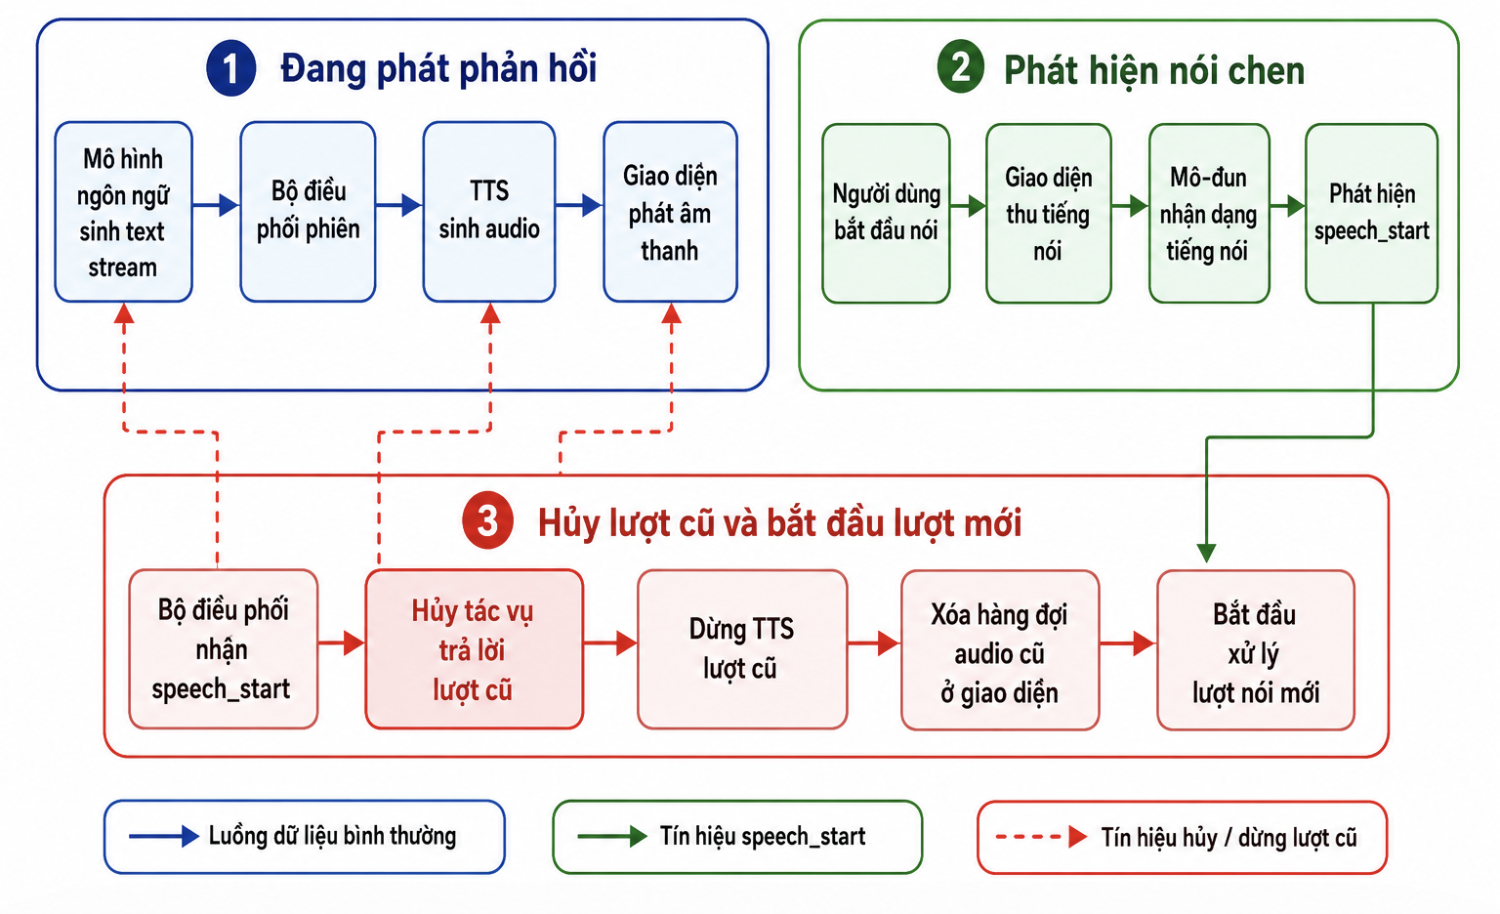
\includegraphics[width=\textwidth,height=0.72\textheight,keepaspectratio]{report_figures/barge_in_flow_compact.png}
    \captionof{figure}{Luồng xử lý barge-in khi người dùng ngắt lời}
    \label{fig:barge-in-flow}
\end{center}
\nopagebreak[4]

Hình~\ref{fig:barge-in-flow} mô tả luồng hủy phản hồi cũ khi người dùng nói chen. Khi mô-đun nhận dạng tiếng nói phát hiện tín hiệu bắt đầu nói, bộ điều phối phiên hủy tác vụ phản hồi hiện tại, yêu cầu TTS dừng tổng hợp theo phiên và thông báo giao diện xóa phần âm thanh đã lập lịch. Sau đó, audio của lượt nói mới được xử lý như một lượt hội thoại mới. Luồng này giúp hạn chế việc âm thanh hoặc văn bản của lượt cũ bị trộn vào lượt mới.

\section{Thiết kế các mô-đun}

\subsection{Giao diện và bộ điều phối phiên}

Giao diện là điểm tiếp xúc trực tiếp giữa người dùng và hệ thống. Thành phần này không thực hiện suy luận nội dung tư vấn, mà tập trung vào hai nhiệm vụ thời gian thực: thu tiếng nói đầu vào và phát âm thanh phản hồi. Ở chiều thu âm, tín hiệu từ micro được lấy liên tục, chuẩn hóa về định dạng thống nhất và chia thành các đoạn ngắn trước khi gửi tới hệ thống. Việc gửi audio theo đoạn ngắn giúp mô-đun nhận dạng tiếng nói phát hiện kịp thời thời điểm người dùng bắt đầu và kết thúc lượt nói, thay vì phải chờ toàn bộ file âm thanh hoàn chỉnh.

Ở chiều phát phản hồi, giao diện nhận các đoạn audio do hệ thống trả về theo luồng. Các đoạn này không được phát rời rạc ngay khi đến, mà được đưa vào hàng đợi phát và lập lịch nối tiếp trên trình duyệt. Cách làm này hạn chế khoảng trống giữa các đoạn âm thanh, đồng thời giúp người dùng nghe câu trả lời như một phản hồi liên tục. Ngoài âm thanh, giao diện cũng nhận các sự kiện trạng thái và văn bản nhận dạng để hiển thị tiến trình hội thoại, chẳng hạn đang nghe, đang xử lý, đang phát phản hồi hoặc transcript của câu hỏi vừa được nhận dạng.

Bộ điều phối phiên là thành phần trung tâm ở phía sau giao diện. Mỗi kết nối hội thoại được gắn với một phiên riêng để tránh trộn dữ liệu giữa các người dùng hoặc giữa các lượt hỏi đáp khác nhau. Bộ điều phối nhận audio từ giao diện, chuyển tới mô-đun nhận dạng tiếng nói và nhận lại văn bản nhận dạng cuối cùng. Sau đó, văn bản này được ghép với lịch sử hội thoại và bản tóm tắt phiên để tạo đầu vào cho mô-đun xử lý hội thoại. Khi mô-đun xử lý hội thoại sinh câu trả lời theo luồng, bộ điều phối nhận các phần văn bản phản hồi, gom chúng thành các đoạn văn bản đủ điều kiện và gửi sang mô-đun tổng hợp tiếng nói.

Một vai trò quan trọng khác của bộ điều phối phiên là duy trì thứ tự và ranh giới dữ liệu trong toàn bộ pipeline. Audio đầu vào, transcript, luồng văn bản phản hồi và luồng audio phản hồi đều phải thuộc đúng phiên hội thoại. Nếu không có lớp điều phối, các mô-đun phía sau có thể vẫn hoạt động độc lập nhưng hệ thống khó bảo đảm rằng câu trả lời, âm thanh và lịch sử hội thoại tương ứng với cùng một lượt người dùng. Vì vậy, bộ điều phối không trực tiếp tạo nội dung tư vấn, nhưng quyết định tính ổn định của trải nghiệm hội thoại.

Hình~\ref{fig:interface-session-flow} minh họa luồng xử lý giữa giao diện và bộ điều phối phiên.

\begin{center}
    \makebox[\textwidth][c]{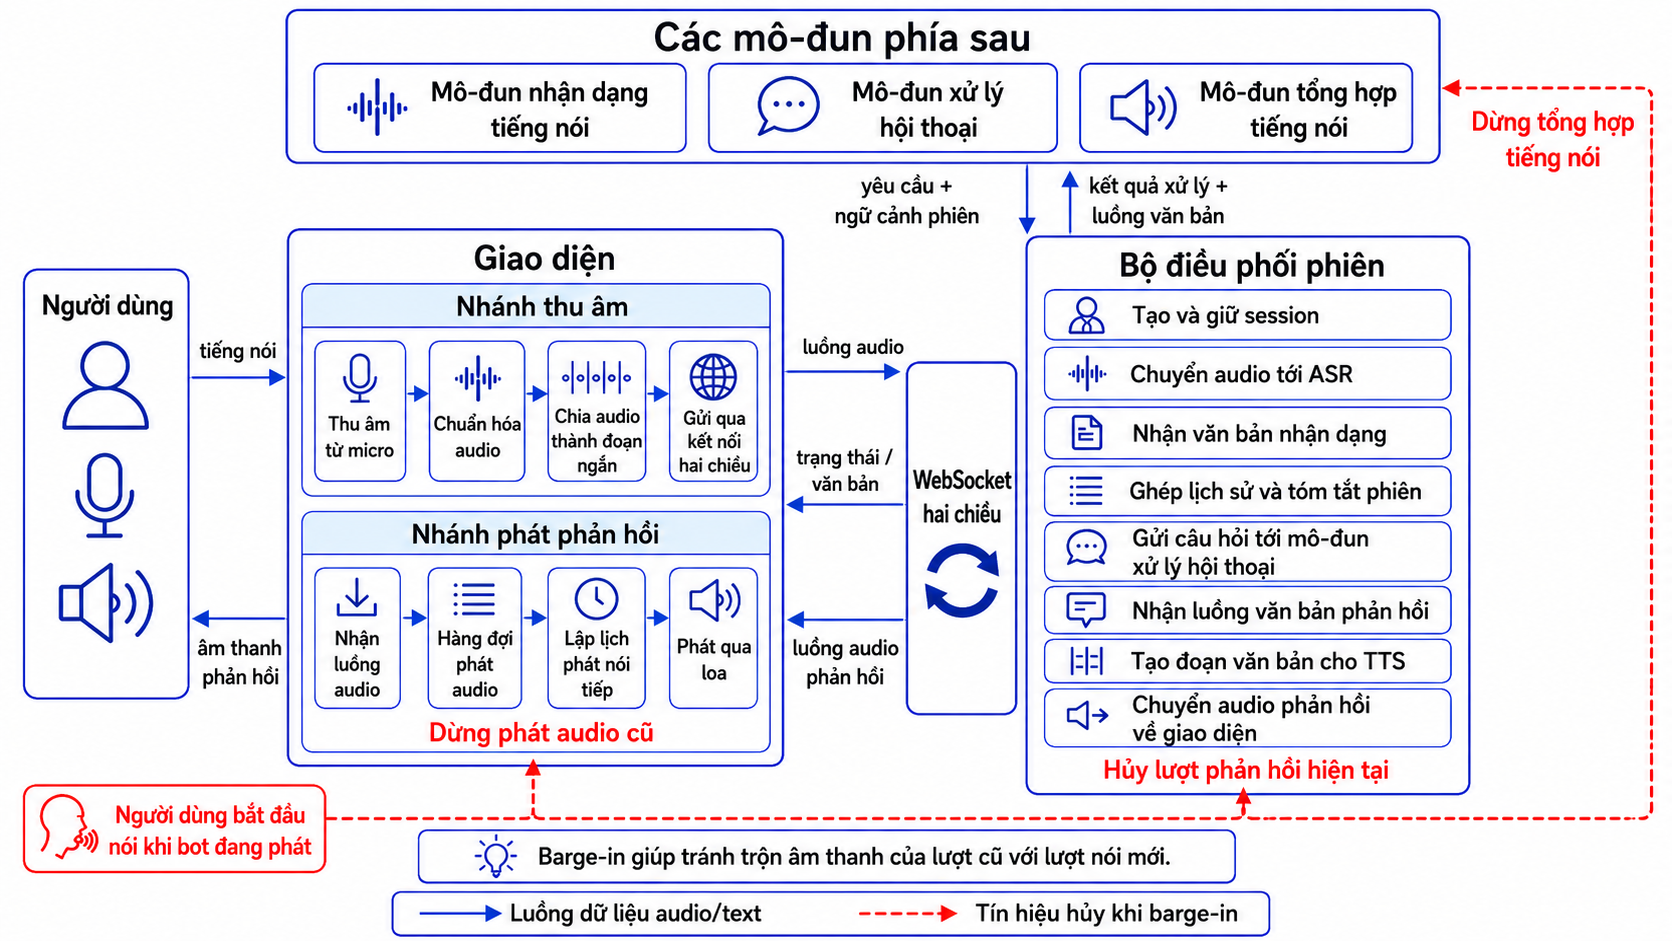
\includegraphics[width=1.18\textwidth]{report_figures/interface_session_flow.png}}
    \captionof{figure}{Luồng xử lý giữa giao diện và bộ điều phối phiên}
    \label{fig:interface-session-flow}
\end{center}
\nopagebreak[4]

Trong Hình~\ref{fig:interface-session-flow}, nhánh thu âm của giao diện nhận tiếng nói từ micro, chuẩn hóa audio, chia thành các đoạn ngắn và gửi qua kết nối hai chiều tới bộ điều phối. Nhánh phát phản hồi thực hiện luồng ngược lại: nhận audio phản hồi từ hệ thống, đưa vào hàng đợi phát, lập lịch phát nối tiếp và phát qua loa. Hai nhánh này cùng tồn tại trong một phiên hội thoại để hệ thống vừa có thể tiếp tục lắng nghe người dùng, vừa phát phản hồi khi có kết quả từ TTS.

Ở phía bộ điều phối, luồng chính bắt đầu bằng việc tạo và giữ phiên hội thoại. Sau đó, audio được chuyển tới ASR để tạo văn bản nhận dạng. Văn bản nhận dạng không được gửi trực tiếp tới LLM một cách độc lập, mà được kết hợp với lịch sử và bản tóm tắt phiên để giữ ngữ cảnh hội thoại. Mô-đun xử lý hội thoại trả về luồng văn bản phản hồi; bộ điều phối chia luồng này thành các đoạn văn bản phù hợp với TTS. Audio sau khi được tổng hợp tiếp tục được chuyển ngược về giao diện để phát cho người dùng.

Luồng barge-in trong Hình~\ref{fig:interface-session-flow} được biểu diễn bằng nét đứt màu đỏ. Khi người dùng bắt đầu nói trong lúc hệ thống đang phát phản hồi, giao diện dừng phần audio cũ đã lập lịch, bộ điều phối hủy lượt phản hồi hiện tại và mô-đun TTS dừng tổng hợp tiếng nói. Cơ chế này giúp hạn chế việc âm thanh của lượt cũ bị trộn với lượt nói mới.

\subsection{Mô-đun nhận dạng tiếng nói}

Mô-đun nhận dạng tiếng nói có nhiệm vụ chuyển luồng audio của người dùng thành văn bản đầu vào cho các bước xử lý phía sau. Trong hệ thống đề xuất, mô-đun này không chỉ chạy một mô hình ASR trên toàn bộ audio, mà còn kết hợp phát hiện hoạt động tiếng nói để xác định ranh giới của từng lượt nói. Cách tổ chức này phù hợp với hệ thống hội thoại vì bộ điều phối cần biết khi nào người dùng bắt đầu nói, khi nào một lượt nói đã kết thúc và khi nào có thể chuyển transcript sang mô-đun xử lý hội thoại.

Đầu vào của mô-đun là luồng audio đã được chuẩn hóa từ bộ điều phối phiên. Audio được đưa qua bước chuẩn hóa để bảo đảm định dạng thống nhất trước khi đi vào bộ phát hiện tiếng nói. Bộ phát hiện tiếng nói xử lý các frame ngắn liên tiếp và duy trì trạng thái của lượt nói hiện tại. Khi phát hiện có tiếng nói, mô-đun phát ra tín hiệu bắt đầu nói. Tín hiệu này không chỉ có ý nghĩa đối với ASR, mà còn được dùng để kích hoạt barge-in nếu hệ thống đang phát câu trả lời cũ.

Trong giai đoạn người dùng đang nói, các frame audio được ghi vào bộ đệm của lượt nói. Bộ đệm này đóng vai trò gom các đoạn audio rời rạc thành một đoạn audio hoàn chỉnh tương ứng với một câu hỏi hoặc một lượt phát ngôn. Khi bộ phát hiện tiếng nói xác định rằng người dùng đã ngừng nói đủ lâu, mô-đun phát ra tín hiệu kết thúc lượt nói và đóng bộ đệm. Đoạn audio hoàn chỉnh sau đó mới được đưa vào mô hình nhận dạng tiếng nói để tạo transcript cuối cùng.

Mô hình nhận dạng trong mô-đun này là mô hình Zipformer--RNN-T. Zipformer đóng vai trò encoder âm học để trích xuất biểu diễn từ chuỗi đặc trưng tiếng nói, còn RNN-T đảm nhiệm cơ chế căn chỉnh và giải mã chuỗi token đầu ra. Kết quả của bước này là transcript cuối cùng của lượt nói, được trả về bộ điều phối phiên. Bộ điều phối sau đó gửi transcript cùng lịch sử và tóm tắt phiên sang mô-đun xử lý hội thoại.

\begin{center}
    \makebox[\textwidth][c]{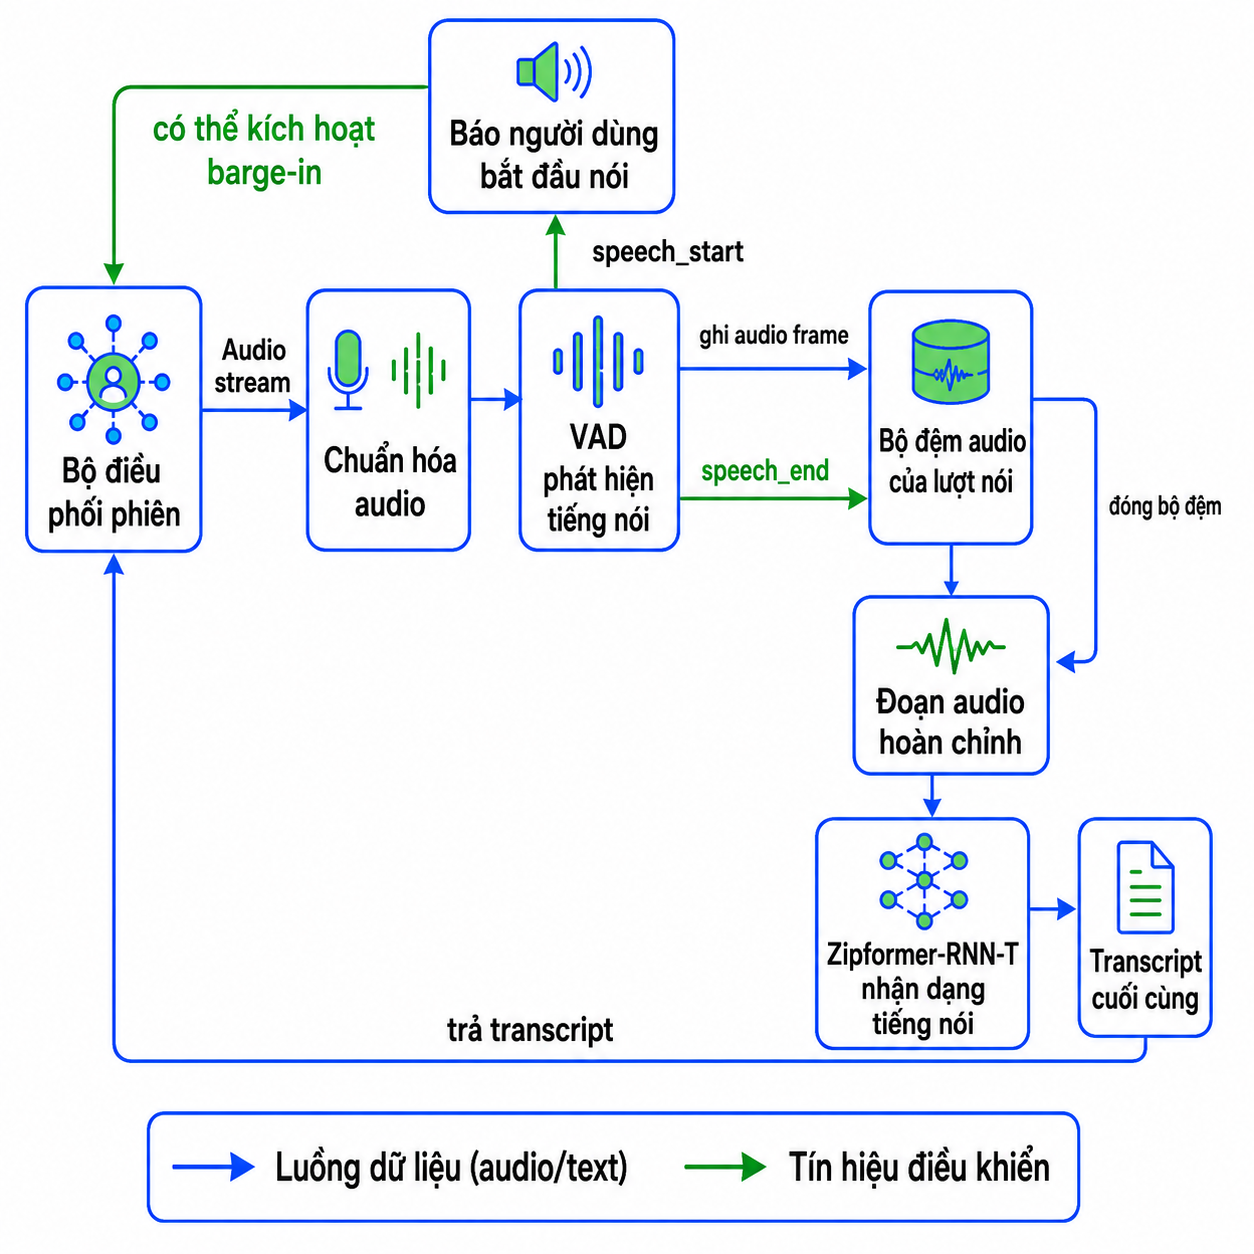
\includegraphics[width=1.12\textwidth,height=0.72\textheight,keepaspectratio]{report_figures/speech_recognition_module_flow.png}}
    \captionof{figure}{Luồng xử lý bên trong mô-đun nhận dạng tiếng nói}
    \label{fig:speech-recognition-module-flow}
\end{center}
\nopagebreak[4]

Hình~\ref{fig:speech-recognition-module-flow} mô tả luồng xử lý bên trong mô-đun nhận dạng tiếng nói. Mũi tên màu xanh dương biểu diễn luồng dữ liệu audio hoặc văn bản, còn mũi tên màu xanh lá biểu diễn tín hiệu điều khiển. Audio stream từ bộ điều phối phiên đi qua bước chuẩn hóa audio, sau đó được đưa vào VAD để phát hiện trạng thái nói. Khi VAD phát hiện người dùng bắt đầu nói, tín hiệu speech\_start được gửi ngược về bộ điều phối để hệ thống có thể dừng phản hồi cũ nếu cần. Khi VAD phát hiện kết thúc lượt nói, tín hiệu speech\_end đóng bộ đệm audio và tạo đoạn audio hoàn chỉnh cho mô hình Zipformer--RNN-T.

Cách tổ chức theo lượt nói giúp hệ thống xác định rõ thời điểm bắt đầu xử lý RAG và tránh gửi các đoạn audio chưa hoàn chỉnh sang mô hình ngôn ngữ. Tuy nhiên, transcript cuối cùng vẫn có thể chứa lỗi ở từ mượn, chữ số hoặc thuật ngữ dinh dưỡng như ``omega ba'', ``can xi'' và ``vitamin đê''. Vì vậy, các bước phía sau cần có cơ chế chuẩn hóa truy vấn và mở rộng thuật ngữ để giảm tác động của lỗi nhận dạng tới truy xuất tri thức.



\subsection{Mô-đun xử lý hội thoại}

Mô-đun xử lý hội thoại nhận transcript từ mô-đun nhận dạng tiếng nói và tạo câu trả lời phù hợp với ngữ cảnh hội thoại. Trong giải pháp đề xuất, mô-đun này không chỉ gọi trực tiếp mô hình ngôn ngữ, mà tổ chức câu hỏi theo quy trình RAG gồm ba pha chính: Retrieval, Augmentation và Generation. Cách tổ chức này giúp câu trả lời được ràng buộc bởi kho tri thức của hệ thống thay vì chỉ dựa vào kiến thức sẵn có của mô hình ngôn ngữ.

Ở pha Retrieval, câu hỏi được kiểm tra phạm vi, chuẩn hóa và mở rộng một số thuật ngữ thường gặp trong chủ đề dinh dưỡng. Sau đó, hệ thống dùng mô hình nhúng để biểu diễn câu hỏi dưới dạng vector và truy xuất một tập đoạn văn bản ứng viên từ kho tri thức vector. Các đoạn ứng viên tiếp tục được đánh giá lại bằng mô hình xếp hạng lại để chọn một số đoạn phù hợp nhất. Việc truy xuất hai bước này nhằm kết hợp ưu điểm của tìm kiếm vector, vốn nhanh và bao phủ rộng, với khả năng đánh giá mức liên quan chi tiết hơn của mô hình xếp hạng lại.

Ở pha Augmentation, các đoạn văn bản đã chọn được ghép với chỉ dẫn hệ thống, lịch sử hội thoại, bản tóm tắt phiên và câu hỏi hiện tại để tạo đầu vào cho mô hình ngôn ngữ. Bước này quyết định cách tri thức bên ngoài được đưa vào quá trình sinh câu trả lời. Nếu ngữ cảnh truy xuất không đủ căn cứ, hệ thống cần trả lời thận trọng thay vì yêu cầu mô hình ngôn ngữ suy diễn vượt quá tài liệu.

Ở pha Generation, mô hình ngôn ngữ sinh câu trả lời dựa trên prompt đã có ngữ cảnh. Do đầu ra sẽ được chuyển sang TTS, câu trả lời cần ngắn gọn, rõ ý, dễ đọc thành tiếng nói và tránh các cấu trúc quá dài. Mô-đun xử lý hội thoại trả văn bản theo luồng để bộ điều phối có thể chuyển dần từng phần sang mô-đun TTS, qua đó giảm thời gian chờ trước âm thanh phản hồi đầu tiên.

\begin{center}
    \makebox[\textwidth][c]{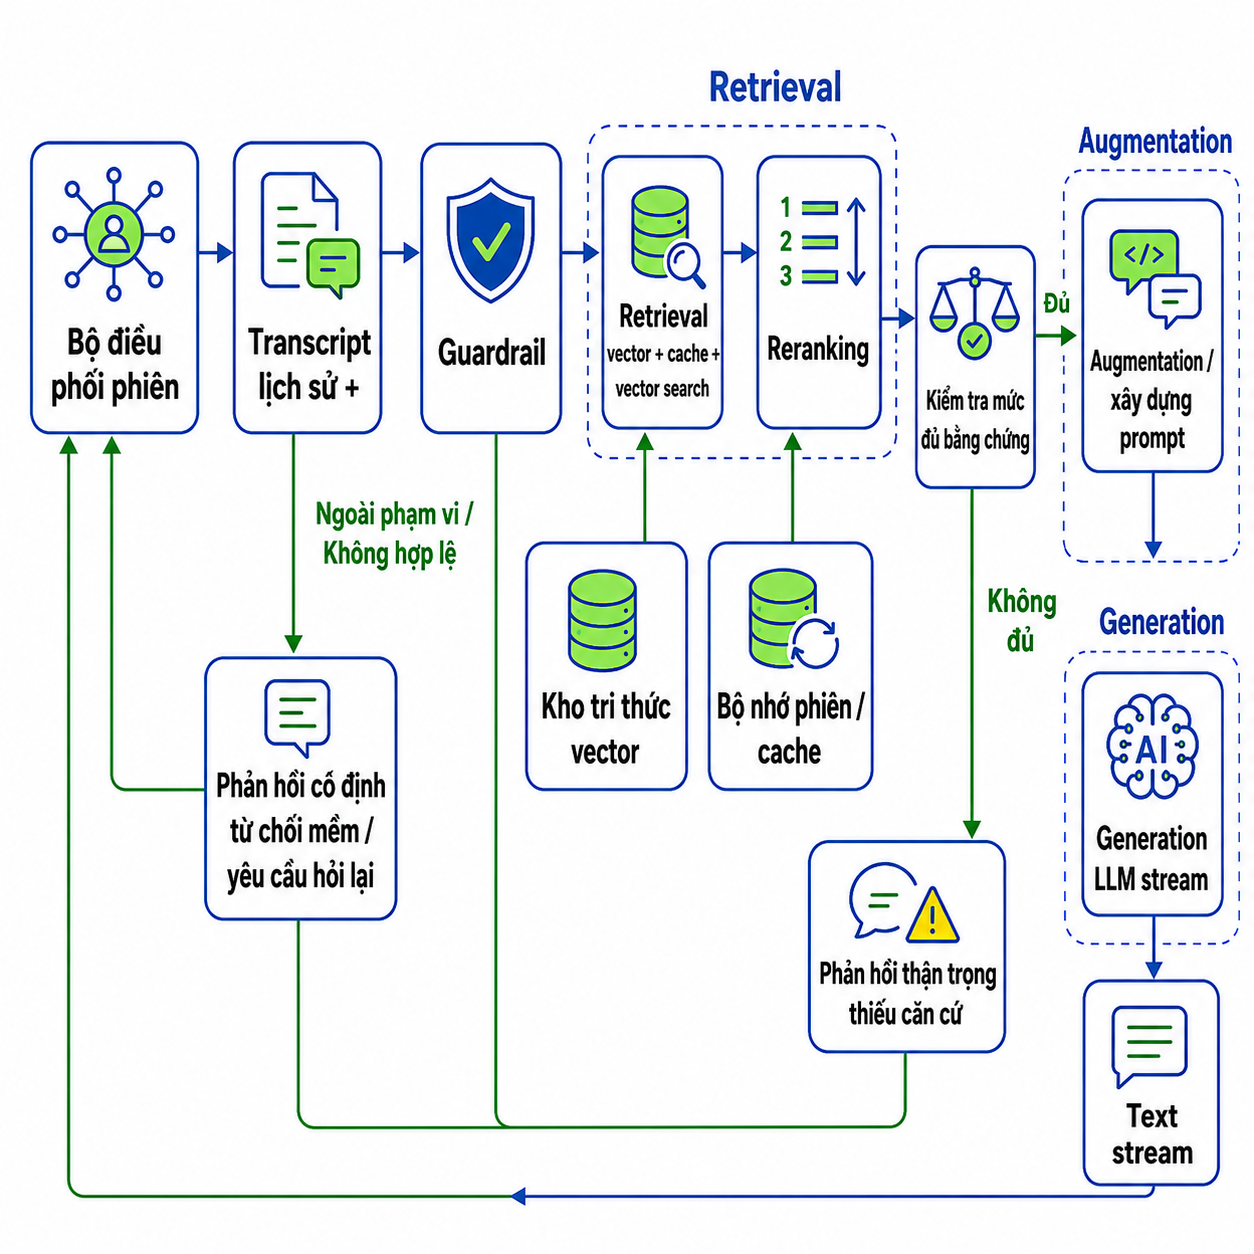
\includegraphics[width=1.12\textwidth,height=0.72\textheight,keepaspectratio]{report_figures/dialogue_module_flow.png}}
    \captionof{figure}{Luồng xử lý bên trong mô-đun xử lý hội thoại}
    \label{fig:dialogue-module-flow}
\end{center}
\nopagebreak[4]

Hình~\ref{fig:dialogue-module-flow} mô tả luồng xử lý bên trong mô-đun xử lý hội thoại ở mức giải pháp. Câu hỏi sau ASR được kiểm tra phạm vi, chuẩn hóa, truy xuất trên kho tri thức, xếp hạng lại và ghép vào prompt cùng ngữ cảnh phiên. Nếu câu hỏi vượt phạm vi hoặc ngữ cảnh không đủ căn cứ, hệ thống có thể trả về phản hồi thận trọng mà không yêu cầu mô hình ngôn ngữ sinh tự do. Nếu câu hỏi hợp lệ và có đủ ngữ cảnh, mô hình ngôn ngữ sinh câu trả lời theo luồng để phục vụ bước tổng hợp tiếng nói phía sau.

\subsection{Mô-đun TTS}

Mô-đun TTS chuyển các đoạn văn bản phản hồi thành tín hiệu âm thanh để phát cho người dùng. Trong hệ thống đề xuất, TTS không nhận toàn bộ câu trả lời sau khi LLM sinh xong, mà nhận từng đoạn văn bản từ bộ điều phối phiên. Cách tổ chức này giúp quá trình tổng hợp tiếng nói có thể bắt đầu sớm hơn, từ đó giảm thời gian người dùng phải chờ trước khi nghe được phần âm thanh đầu tiên.

Đầu vào của mô-đun là một đoạn văn bản đã được bộ điều phối làm sạch và chia tại các ranh giới tương đối tự nhiên. Việc chia đoạn được thực hiện trước TTS nhằm tránh gửi những mảnh văn bản quá ngắn hoặc bị cắt giữa từ. Nếu đoạn quá ngắn, TTS có thể tạo nhịp đọc thiếu tự nhiên; nếu đoạn quá dài, thời gian chờ trước chunk âm thanh đầu tiên sẽ tăng. Vì vậy, kích thước đoạn văn bản là một tham số ảnh hưởng trực tiếp tới cân bằng giữa độ trễ và chất lượng cảm nhận.

\begin{center}
    \makebox[\textwidth][c]{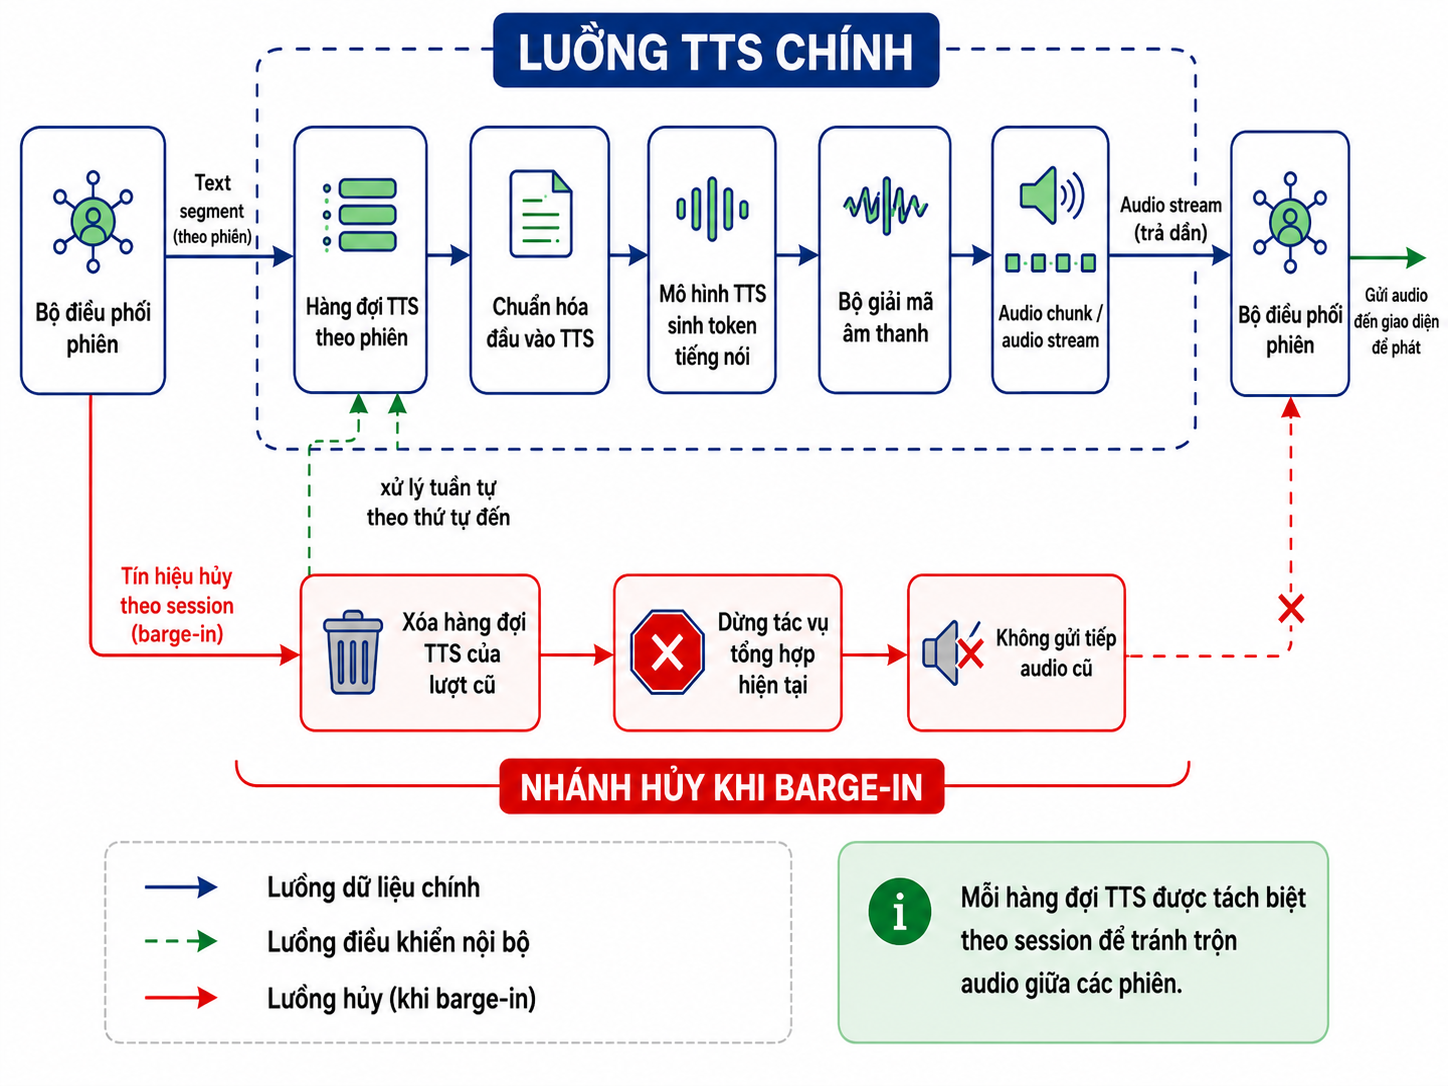
\includegraphics[width=1.12\textwidth,height=0.72\textheight,keepaspectratio]{report_figures/tts_module_flow.png}}
    \captionof{figure}{Luồng xử lý bên trong mô-đun TTS}
    \label{fig:tts-module-flow}
\end{center}
\nopagebreak[4]

Hình~\ref{fig:tts-module-flow} mô tả luồng xử lý bên trong mô-đun TTS. Sau khi nhận một đoạn văn bản, mô-đun kiểm tra cache âm thanh theo nội dung văn bản và cấu hình giọng đọc. Nếu cache có kết quả, hệ thống có thể trả lại các đoạn PCM đã lưu mà không cần chạy lại mô hình tổng hợp. Nếu cache không có kết quả phù hợp, đoạn văn bản được đưa vào bộ tổng hợp tiếng nói để sinh audio stream.

Mô hình TTS được sử dụng theo cơ chế sinh luồng. Văn bản đầu vào được chuyển thành chuỗi token tiếng nói; khi số token mới sinh ra đạt một ngưỡng nhất định, bộ giải mã âm thanh sẽ tái tạo một đoạn waveform tương ứng và trả ra ngay cho bộ điều phối. Trong cấu hình hiện tại, mỗi lần giải mã sử dụng một cửa sổ gồm các token mới, một phần ngữ cảnh quá khứ và một phần ngữ cảnh tương lai ngắn. Ngữ cảnh quá khứ giúp đoạn âm thanh mới nối mạch với phần đã phát trước đó, còn ngữ cảnh tương lai giúp giảm lỗi phát âm hoặc ngắt nhịp ở biên đoạn.

Cụ thể, cơ chế streaming của VieNeu-TTS duy trì một bộ nhớ token đã sinh và giải mã âm thanh theo từng cửa sổ. Mỗi cửa sổ lấy thêm một số token nhìn lại phía trước và phía sau so với phần âm thanh cần phát. Sau khi giải mã, các đoạn waveform được ghép bằng overlap-add tuyến tính để làm mượt ranh giới giữa các đoạn. Phần âm thanh ổn định sau xử lý được chuyển thành PCM int16, đơn kênh, tần số lấy mẫu 24 kHz và gửi dần về bộ điều phối phiên. Bộ điều phối sau đó chuyển các đoạn PCM này về giao diện để phát nối tiếp.

Do backend TTS hiện tại chưa được giả định là an toàn khi chạy nhiều suy luận song song trên cùng một tiến trình, mô-đun giới hạn số tác vụ tổng hợp đồng thời. Cách làm này ưu tiên tính ổn định của demo và tránh tình trạng nhiều lượt tổng hợp cùng truy cập trạng thái nội bộ của mô hình. Khi cần mở rộng số người dùng đồng thời, hướng phù hợp hơn là nhân bản tiến trình TTS hoặc tách nhiều worker thay vì tăng tùy tiện số luồng suy luận trong cùng một tiến trình.

Khi người dùng ngắt lời trong lúc hệ thống đang phát, bộ điều phối gửi tín hiệu hủy theo phiên. Mô-đun TTS dừng tổng hợp phần âm thanh của lượt cũ và không tiếp tục trả các đoạn âm thanh đã không còn phù hợp. Cơ chế này giúp hạn chế việc phản hồi cũ bị trộn với lượt hội thoại mới.

\subsection{Kho tri thức và bộ nhớ phiên}

Kho tri thức và bộ nhớ phiên là hai thành phần lưu trữ có vai trò khác nhau trong hệ thống. Kho tri thức lưu các thông tin nền đã được chuẩn bị trước để phục vụ truy xuất, trong khi bộ nhớ phiên lưu trạng thái hội thoại ngắn hạn của từng người dùng. Việc tách hai nhóm lưu trữ này giúp hệ thống vừa có nguồn tri thức ổn định để sinh câu trả lời có căn cứ, vừa duy trì được mạch hội thoại giữa các lượt hỏi đáp liên tiếp.

\begin{center}
    \makebox[\textwidth][c]{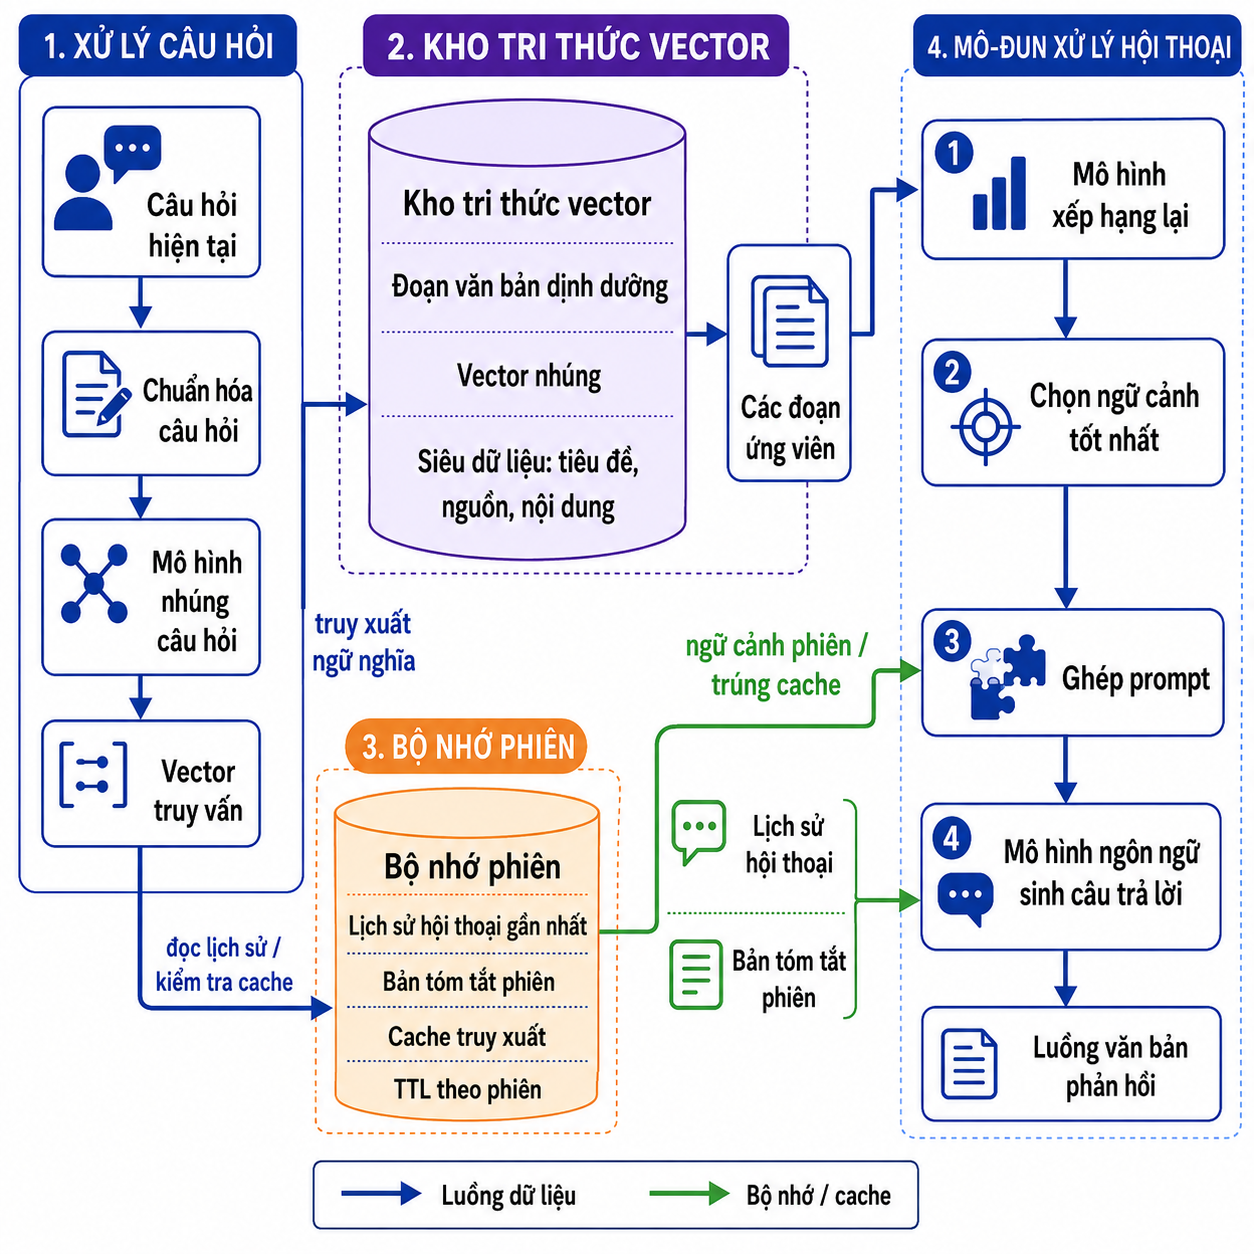
\includegraphics[width=1.12\textwidth,height=0.72\textheight,keepaspectratio]{report_figures/knowledge_session_memory_flow.png}}
    \captionof{figure}{Quan hệ giữa kho tri thức, bộ nhớ phiên và đầu vào mô hình ngôn ngữ}
    \label{fig:knowledge-session-memory-flow}
\end{center}
\nopagebreak[4]
\FloatBarrier

Hình~\ref{fig:knowledge-session-memory-flow} minh họa cách câu hỏi hiện tại, kho tri thức vector và bộ nhớ phiên cùng tham gia vào quá trình tạo đầu vào cho mô hình ngôn ngữ. Kho tri thức cung cấp các đoạn văn bản có căn cứ, còn bộ nhớ phiên cung cấp lịch sử, bản tóm tắt và cache truy xuất để giữ mạch hội thoại và giảm lặp lại các bước xử lý tốn thời gian.

Kho tri thức được tổ chức theo đơn vị đoạn văn bản thay vì toàn bộ bài viết. Mỗi bài viết sau khi thu thập và làm sạch được chia thành nhiều đoạn nhỏ. Một đoạn phù hợp cần đủ ngắn để truy xuất chính xác theo câu hỏi, nhưng vẫn đủ dài để giữ được ngữ cảnh cần thiết cho mô hình ngôn ngữ. Nếu đoạn quá dài, kết quả truy xuất có thể chứa nhiều thông tin thừa; nếu đoạn quá ngắn, mô hình ngôn ngữ có thể thiếu căn cứ để tạo câu trả lời đầy đủ. Vì vậy, phân đoạn tài liệu là bước ảnh hưởng trực tiếp đến chất lượng của pha Retrieval.

Mỗi đoạn văn bản trong kho tri thức được lưu cùng hai nhóm thông tin. Nhóm thứ nhất là nội dung phục vụ truy xuất và sinh câu trả lời, bao gồm tiêu đề, phần văn bản chính và đoạn văn bản sau xử lý. Nhóm thứ hai là thông tin mô tả, bao gồm nguồn, địa chỉ bài viết, chuyên mục hoặc các trường hỗ trợ truy vết. Các thông tin mô tả này không nhất thiết được đưa trực tiếp vào câu trả lời, nhưng có ý nghĩa trong quá trình kiểm tra dữ liệu, đánh giá kết quả truy xuất và cập nhật kho tri thức.

Để phục vụ truy xuất ngữ nghĩa, mỗi đoạn văn bản được mã hóa bằng mô hình nhúng thành một vector. Khi người dùng đặt câu hỏi, câu hỏi sau chuẩn hóa cũng được mã hóa thành vector truy vấn. Hệ thống so sánh vector truy vấn với các vector trong kho tri thức để tìm ra một tập đoạn văn bản ứng viên có ý nghĩa gần với câu hỏi. Đây là bước truy xuất ban đầu, có nhiệm vụ thu hẹp không gian tìm kiếm từ toàn bộ kho tri thức xuống một số đoạn có khả năng liên quan.

Tuy nhiên, kết quả truy xuất theo vector chưa đủ để đưa trực tiếp vào đầu vào của mô hình ngôn ngữ. Một số đoạn có thể gần về mặt từ vựng hoặc chủ đề nhưng không trả lời đúng trọng tâm câu hỏi. Vì vậy, các đoạn ứng viên tiếp tục được đưa qua mô hình xếp hạng lại. Mô hình này đánh giá trực tiếp mức phù hợp giữa câu hỏi và từng đoạn văn bản, sau đó chọn ra một số đoạn tốt nhất làm ngữ cảnh. Cách xử lý hai bước này giúp cân bằng giữa tốc độ truy xuất của kho vector và độ chính xác của bước lựa chọn ngữ cảnh.

Bên cạnh kho tri thức, bộ nhớ phiên lưu các thông tin gắn với một phiên hội thoại cụ thể. Thành phần này gồm lịch sử hội thoại gần nhất, bản tóm tắt các lượt cũ hơn và một số dữ liệu cache phục vụ tối ưu truy xuất. Lịch sử gần nhất giữ lại nguyên văn một số lượt hỏi đáp mới xảy ra để xử lý các câu hỏi nối tiếp. Bản tóm tắt phiên giúp duy trì các thông tin quan trọng trong hội thoại dài hơn, chẳng hạn nhóm đối tượng, mục tiêu ăn uống, tình trạng liên quan hoặc chủ đề đã trao đổi, mà không làm đầu vào của mô hình ngôn ngữ tăng quá dài.

Cache truy xuất được dùng để tránh lặp lại các bước tốn thời gian khi câu hỏi đã chuẩn hóa xuất hiện lại hoặc có dạng rất gần với câu hỏi trước đó. Thay vì mã hóa lại câu hỏi, tìm kiếm lại trong kho tri thức và xếp hạng lại toàn bộ các đoạn ứng viên, hệ thống có thể tái sử dụng tập ngữ cảnh đã chọn nếu điều kiện cache phù hợp. Cache này chỉ lưu kết quả truy xuất hoặc ngữ cảnh đã chọn, không cố định toàn bộ câu trả lời cuối cùng. Lý do là câu trả lời còn phụ thuộc vào lịch sử của phiên hiện tại, cách người dùng đặt câu hỏi và các ràng buộc trong prompt tại thời điểm sinh.

Khi xây dựng đầu vào cho mô hình ngôn ngữ, mô-đun xử lý hội thoại kết hợp ba nhóm thông tin: câu hỏi hiện tại, ngữ cảnh truy xuất từ kho tri thức và ngữ cảnh hội thoại từ bộ nhớ phiên. Câu hỏi hiện tại xác định yêu cầu cần trả lời; ngữ cảnh truy xuất cung cấp bằng chứng nội dung; lịch sử và bản tóm tắt phiên giúp hiểu các câu hỏi nối tiếp. Việc ghép ba nhóm thông tin này là pha Augmentation trong pipeline RAG, nhằm giúp mô hình ngôn ngữ sinh câu trả lời bám vào tài liệu thay vì chỉ dựa vào tri thức tham số.

Các dữ liệu trong bộ nhớ phiên cần có thời gian tồn tại để tránh tích lũy vô hạn và hạn chế lưu các thông tin không còn cần thiết. Lịch sử hội thoại và bản tóm tắt nên gắn với vòng đời của phiên, trong khi cache truy xuất có thể tồn tại lâu hơn nếu không chứa thông tin cá nhân nhạy cảm. Thiết kế này tách rõ hai mục tiêu: duy trì ngữ cảnh hội thoại cho trải nghiệm hỏi đáp liên tục và tái sử dụng kết quả truy xuất để giảm độ trễ cho các câu hỏi thường gặp.

\section{Chiến thuật streaming và tối ưu độ trễ}

Nếu pipeline hoạt động tuần tự, hệ thống phải chờ mô hình ngôn ngữ sinh xong toàn bộ câu trả lời rồi mới bắt đầu TTS. Giải pháp đề xuất cho phép quá trình sinh văn bản và tổng hợp tiếng nói chồng lấp thời gian. Mô hình ngôn ngữ đóng vai trò producer tạo các phần văn bản, TTS là consumer tổng hợp từng đoạn, còn bộ điều phối duy trì hàng đợi bất đồng bộ giữa hai thành phần.

Văn bản được phân đoạn ở hai mức. Trước hết, mô-đun xử lý hội thoại tạo các phần văn bản theo dấu kết thúc câu hoặc theo ngưỡng ký tự. Bộ điều phối tiếp tục cộng dồn các phần này trong một bộ đệm trước khi gửi sang TTS. Bộ điều phối ưu tiên tách sau dấu câu khi bộ đệm đạt ngưỡng tối thiểu; nếu bộ đệm đạt ngưỡng tối đa mà chưa gặp dấu câu phù hợp, toàn bộ nội dung hiện có được chuyển sang TTS để tránh chờ quá lâu. Hàng đợi văn bản gửi TTS được giới hạn kích thước để tốc độ sinh văn bản không vượt quá xa tốc độ tổng hợp âm thanh.

Với xử lý tuần tự, thời gian đến âm thanh đầu tiên có thể biểu diễn gần đúng bởi:

\begin{equation}
    T_{\mathrm{seq}}
    =
    T_{\mathrm{ASR}}
    +T_{\mathrm{RAG}}
    +T_{\mathrm{LLM\text{-}full}}
    +T_{\mathrm{TTS\text{-}first}}.
\end{equation}

Khi sử dụng streaming, hệ thống chỉ cần chờ phần văn bản đầu tiên đủ điều kiện:

\begin{equation}
    T_{\mathrm{stream}}
    =
    T_{\mathrm{ASR}}
    +T_{\mathrm{RAG}}
    +T_{\mathrm{LLM\text{-}first\text{-}chunk}}
    +T_{\mathrm{TTS\text{-}first}}.
\end{equation}

Do \(T_{\mathrm{LLM\text{-}first\text{-}chunk}}\) nhỏ hơn thời gian sinh toàn bộ câu trả lời, chiến thuật này làm giảm Time-to-First-Audio mà không yêu cầu bỏ bớt bước truy xuất. Tuy nhiên, đoạn quá nhỏ có thể làm giọng đọc rời rạc và tăng số lần tổng hợp, còn đoạn quá lớn làm tăng thời gian chờ. Vì vậy, ảnh hưởng của ngưỡng chia đoạn được đánh giá thực nghiệm trong Chương 5.


\chapter{PHÁT TRIỂN HỆ THỐNG VOICEBOT TƯ VẤN DINH DƯỠNG}

\section{Kiến trúc hệ thống voicebot}

Chương này trình bày cách hiện thực giải pháp đã nêu ở Chương 3 thành một hệ thống có thể chạy thử và đo đạc. Khác với Chương 3, nội dung ở đây đi vào các công nghệ, mô hình và cơ chế phần mềm cụ thể được sử dụng trong từng mô-đun. Hệ thống được tổ chức theo pipeline gồm giao diện, Gateway, ASR, mô-đun xử lý hội thoại, mô hình ngôn ngữ, TTS, Qdrant và Redis. Các thành phần trao đổi với nhau bằng HTTP, WebSocket và cơ chế streaming, trong đó Gateway giữ vai trò điều phối phiên hội thoại.

Ở mức triển khai, giao diện sử dụng React, Vite và Web Audio API để thu tiếng nói, hiển thị trạng thái hội thoại và phát âm thanh phản hồi \cite{react,vite,webaudio}. Gateway được xây dựng bằng FastAPI, duy trì kết nối hai chiều với giao diện, nhận audio đầu vào, chuyển audio sang ASR, nhận transcript, gọi mô-đun xử lý hội thoại và chuyển văn bản sang TTS \cite{fastapi}. ASR sử dụng Sherpa-ONNX, Silero VAD và checkpoint Zipformer--RNN-T tiếng Việt \cite{sherpaonnx,silerovad,zipformer6000h}. Mô-đun xử lý hội thoại sử dụng Qwen-3-4b-2507 cho pha sinh câu trả lời, AITeamVN/Vietnamese\_Embedding cho mô hình nhúng, thanhtantran/Vietnamese\_Reranker cho mô hình xếp hạng lại và Qdrant cho truy xuất vector \cite{qwen3modelcard,vietembedding,vietreranker,qdrant}. TTS sử dụng VieNeu-TTS để tổng hợp tiếng nói tiếng Việt thành PCM 24~kHz \cite{vieneutts}. Redis được dùng cho lịch sử phiên, bản tóm tắt hội thoại và cache truy xuất \cite{redis}.

Các thành phần được đóng gói bằng Docker Compose \cite{dockercompose}. Mỗi thành phần có Dockerfile riêng để tách môi trường phụ thuộc, tránh xung đột thư viện giữa các mô-đun có yêu cầu runtime khác nhau. Cấu hình chính khởi động Gateway, ASR, mô-đun xử lý hội thoại, TTS, Qdrant, Redis và giao diện. Cấu hình GPU bổ sung mô hình ngôn ngữ chạy qua máy chủ tương thích OpenAI API, đồng thời cho phép ASR, mô hình nhúng, mô hình xếp hạng lại và TTS sử dụng CUDA khi môi trường hỗ trợ \cite{cuda}. Mỗi thành phần chính có healthcheck để Gateway chỉ khởi động sau khi các mô-đun phụ thuộc sẵn sàng, giúp tránh lỗi kết nối trong giai đoạn khởi động hệ thống.

\begin{figure}[H]
    \centering
    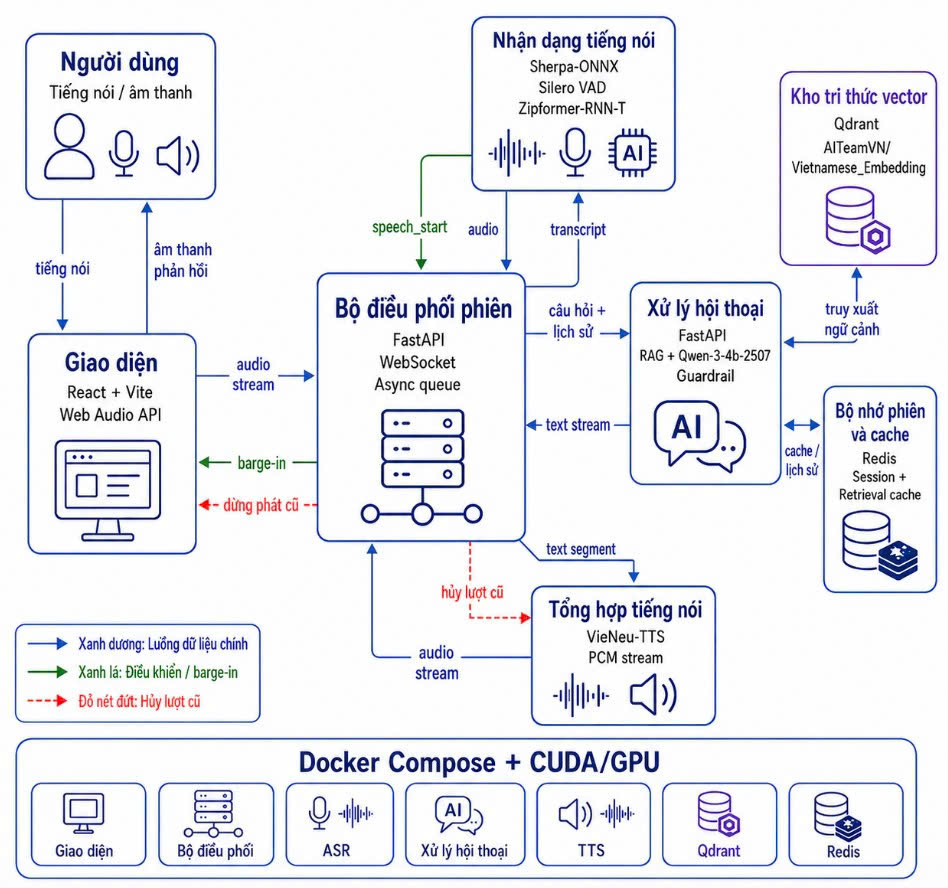
\includegraphics[width=\textwidth]{report_figures/chapter4_system_architecture.png}
    \caption{Kiến trúc triển khai của hệ thống voicebot với các công nghệ sử dụng}
    \label{fig:chapter4-system-architecture}
\end{figure}

Hình~\ref{fig:chapter4-system-architecture} mô tả kiến trúc triển khai với các công nghệ cụ thể. Gateway là điểm vào chính của pipeline thời gian thực. Các mô-đun ASR, xử lý hội thoại và TTS được triển khai tách biệt để cô lập môi trường thư viện, mô hình và tài nguyên tính toán. Qdrant lưu kho tri thức dạng vector, còn Redis lưu dữ liệu có vòng đời ngắn hơn như phiên hội thoại, bản tóm tắt và kết quả truy xuất đã xếp hạng lại. Bảng~\ref{tab:system-technologies} tóm tắt công nghệ sử dụng trong từng thành phần.

\begin{table}[H]
    \centering
    \normalsize
    \renewcommand{\arraystretch}{1.3}
    \begin{tabularx}{\textwidth}{|>{\RaggedRight\arraybackslash}p{3.0cm}|>{\RaggedRight\arraybackslash}p{4.8cm}|>{\RaggedRight\arraybackslash}X|}
        \hline
        \textbf{Thành phần} & \textbf{Công nghệ chính}                        & \textbf{Vai trò trong hệ thống}                                             \\
        \hline
        Giao diện           & React, Vite, Web Audio API                      & Thu audio, gửi PCM 16~kHz, hiển thị transcript và phát PCM 24~kHz phản hồi. \\
        \hline
        Gateway             & FastAPI, WebSocket, hàng đợi bất đồng bộ        & Quản lý session, điều phối audio, transcript, text stream và audio stream.  \\
        \hline
        ASR                 & Sherpa-ONNX, Silero VAD, Zipformer--RNN-T       & Phát hiện lượt nói, tạo đoạn audio hoàn chỉnh và nhận dạng tiếng Việt.      \\
        \hline
        Xử lý hội thoại     & FastAPI, Qwen-3-4b-2507, RAG                    & Guardrail, chuẩn hóa truy vấn, truy xuất, xếp hạng lại và sinh câu trả lời. \\
        \hline
        Kho tri thức        & Qdrant, AITeamVN/\newline Vietnamese\_Embedding & Lưu vector và phục vụ truy xuất ngữ nghĩa trên dữ liệu dinh dưỡng.          \\
        \hline
        Lưu trạng thái      & Redis                                           & Lưu lịch sử phiên, bản tóm tắt hội thoại và cache truy xuất.                \\
        \hline
        TTS                 & VieNeu-TTS                                      & Tổng hợp text segment thành audio PCM int16, đơn kênh, 24~kHz.              \\
        \hline
        Triển khai          & Docker Compose, CUDA                            & Tách môi trường thư viện, cấu hình healthcheck và hỗ trợ tăng tốc trên GPU. \\
        \hline
    \end{tabularx}
    \caption{Công nghệ sử dụng trong hệ thống voicebot}
    \label{tab:system-technologies}
\end{table}

\section{Thiết kế chi tiết}

\subsection{Giao diện}

Giao diện đảm nhiệm hai luồng xử lý đồng thời: thu tiếng nói đầu vào và phát âm thanh phản hồi. Khi người dùng bắt đầu phiên hội thoại, trình duyệt xin quyền micro và tạo một ngữ cảnh âm thanh ở tần số 16~kHz, một kênh. Tín hiệu thu được được đưa qua một bộ xử lý audio chạy trong audio thread của trình duyệt. Bộ xử lý này gom mẫu âm thanh thành từng đoạn 100 ms, tương ứng 1600 mẫu ở 16~kHz, sau đó chuyển biên độ dạng số thực sang PCM int16 và gửi từng đoạn qua kết nối hai chiều tới Gateway.

\begin{figure}[H]
    \centering
    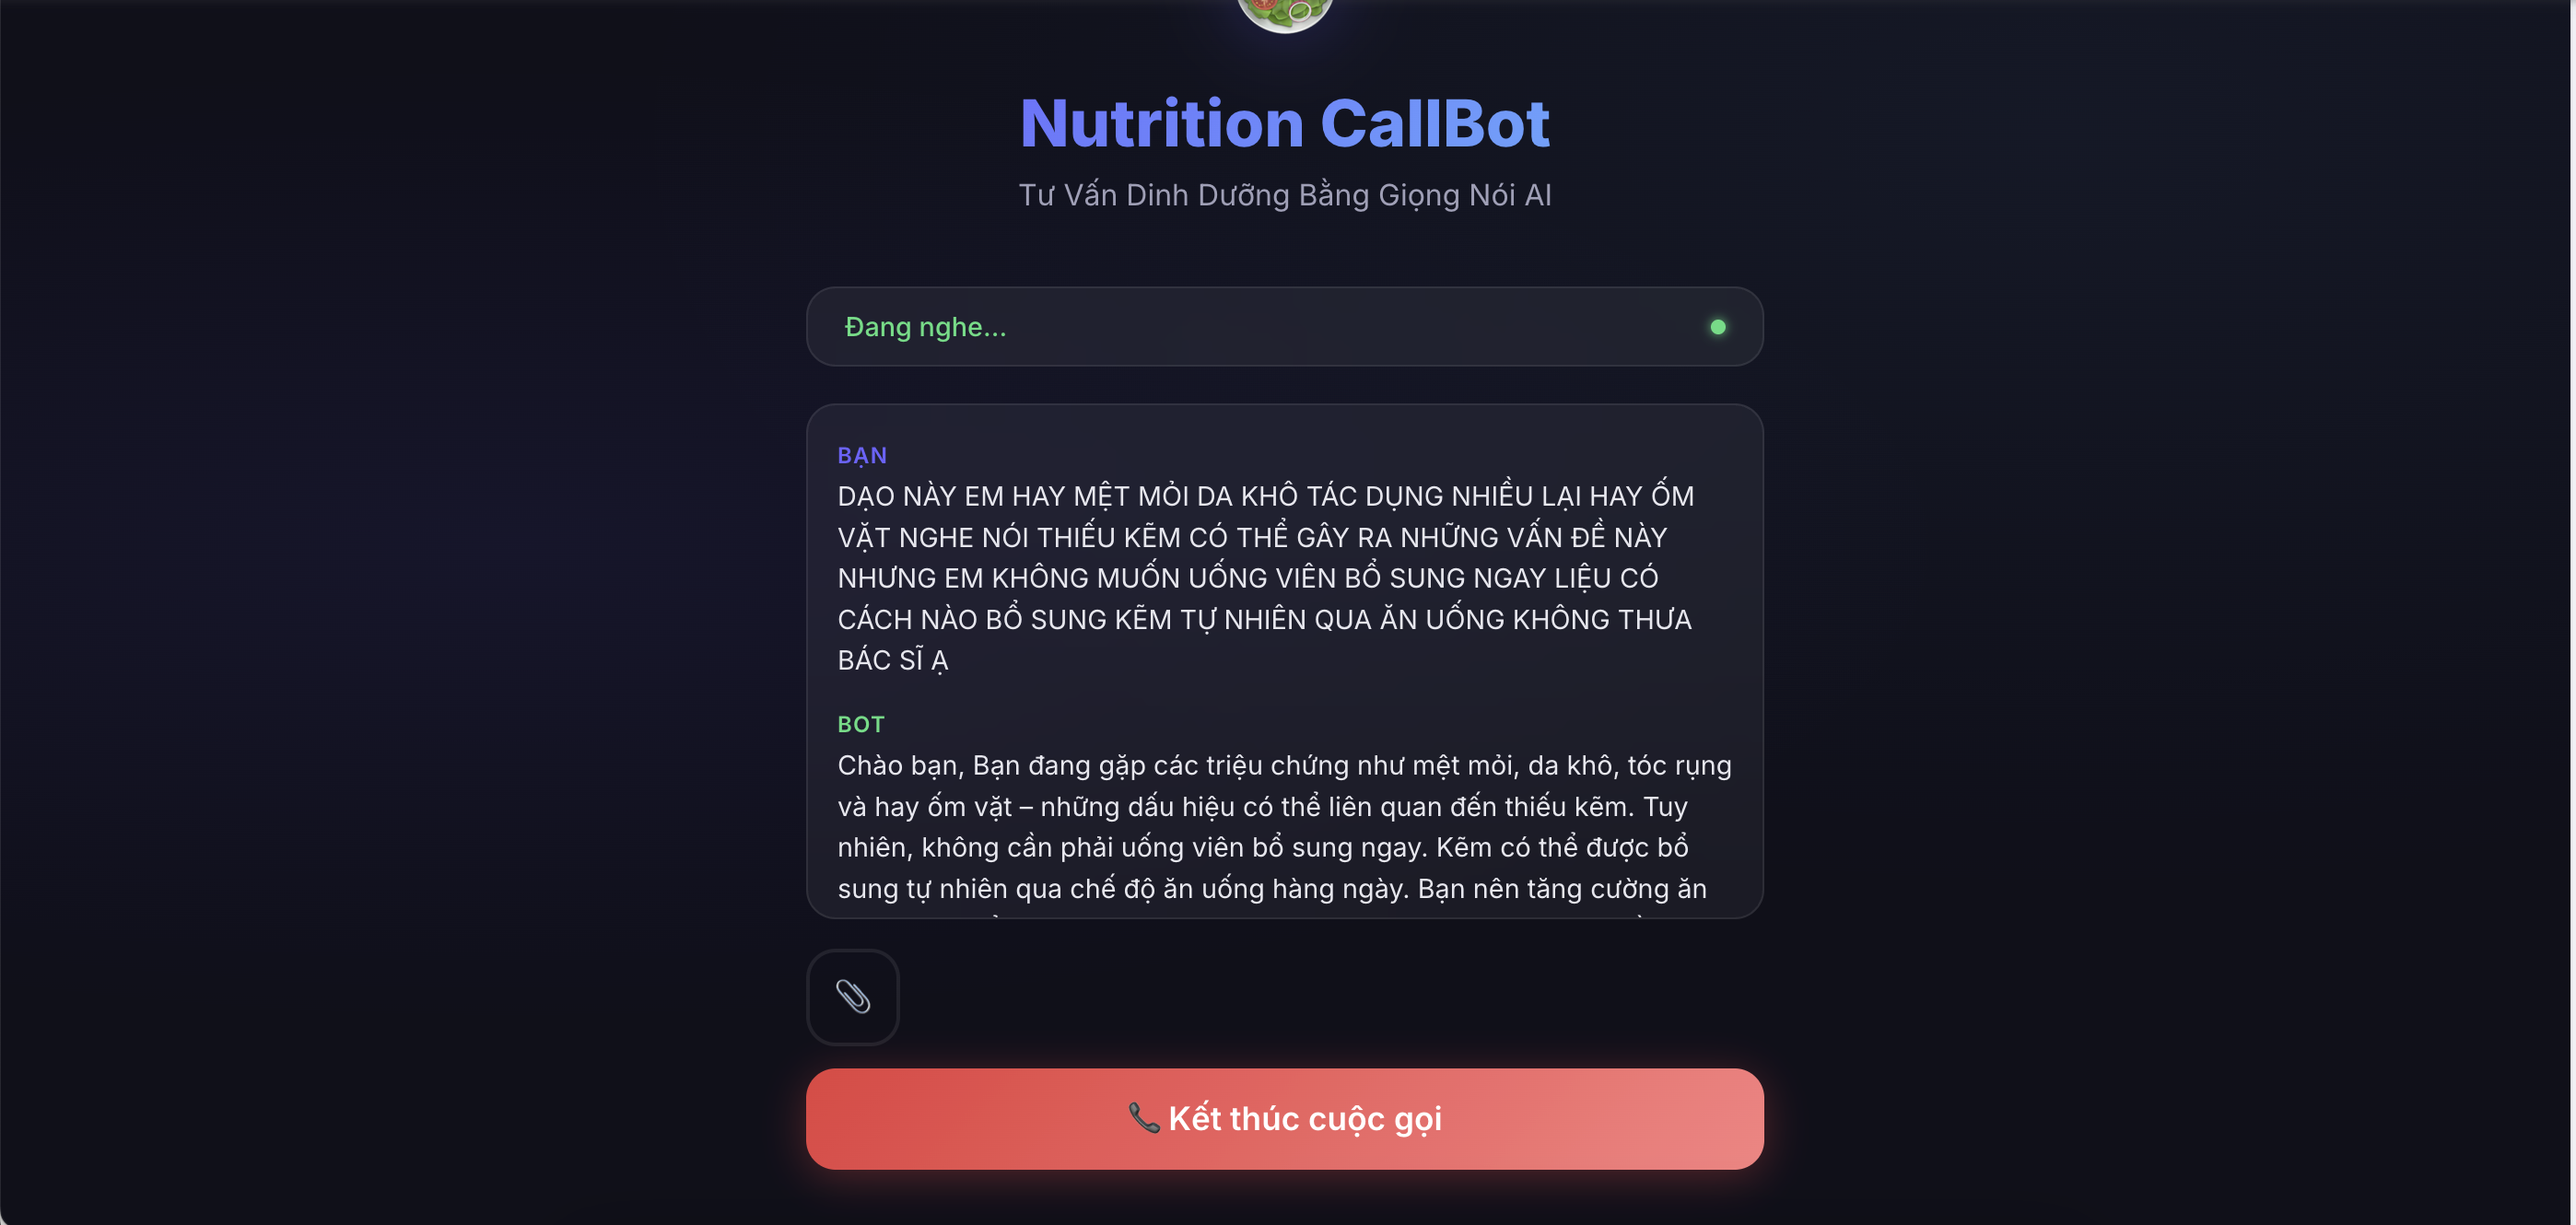
\includegraphics[width=\textwidth]{report_figures/chapter4_interface_demo.png}
    \caption{Giao diện thử nghiệm của hệ thống voicebot tư vấn dinh dưỡng}
    \label{fig:chapter4-interface-demo}
\end{figure}

Hình~\ref{fig:chapter4-interface-demo} minh họa giao diện thử nghiệm của hệ thống trong một phiên hỏi đáp. Giao diện hiển thị trạng thái phiên, transcript của người dùng, nội dung phản hồi dạng văn bản của hệ thống và nút kết thúc cuộc gọi. Trong quá trình demo, phần văn bản giúp kiểm tra nhanh kết quả nhận dạng và câu trả lời, còn kênh tương tác chính vẫn là thu tiếng nói và phát âm thanh phản hồi.

Cách gửi audio theo đoạn ngắn giúp hệ thống phía sau phát hiện được tín hiệu bắt đầu nói và kết thúc lượt nói mà không cần chờ người dùng tải lên một file âm thanh hoàn chỉnh. Trình duyệt cũng bật các tùy chọn giảm nhiễu và khử vọng ở mức thiết bị khi xin quyền micro. Dữ liệu gửi đi ở dạng nhị phân, còn các thông báo trạng thái như transcript, trạng thái đang nghe, đang xử lý hoặc đang phát phản hồi được nhận ở dạng JSON.

Ở chiều phát âm thanh, giao diện nhận các đoạn PCM int16 24~kHz từ Gateway. Mỗi đoạn được chuyển thành AudioBuffer một kênh và được lập lịch phát bằng một biến thời gian kế tiếp. Nếu đoạn mới đến khi đoạn trước vẫn đang phát, giao diện đặt thời điểm bắt đầu của đoạn mới ngay sau đoạn trước; nếu hàng đợi đã rỗng, đoạn mới được phát từ thời điểm hiện tại. Cách lập lịch này giúp giảm khoảng trống giữa các audio chunk và tạo cảm giác phản hồi liền mạch hơn.

Khi hệ thống bắt đầu một câu trả lời mới, giao diện xóa lịch phát cũ để tránh âm thanh từ lượt trước tiếp tục phát. Khi nhận sự kiện người dùng ngắt lời, giao diện dừng các AudioBufferSource đã lập lịch, xóa hàng đợi phát và chuyển trạng thái hiển thị sang đang xử lý lượt mới. Nhờ đó, giao diện không chỉ là lớp hiển thị mà còn tham gia trực tiếp vào việc bảo đảm ranh giới giữa các lượt hội thoại.

\subsection{Gateway và điều phối phiên}

Gateway là lớp điều phối trung tâm của pipeline. Mỗi kết nối từ giao diện được gán một mã phiên riêng. Mã phiên này được dùng xuyên suốt quá trình chuyển audio sang ASR, gửi transcript sang mô-đun xử lý hội thoại, gọi TTS và lưu lịch sử hội thoại. Việc gắn mọi dữ liệu với mã phiên giúp hạn chế việc văn bản hoặc âm thanh của hai lượt hội thoại bị trộn lẫn.

Khi phiên bắt đầu, Gateway tạo một worker riêng để duy trì kết nối streaming tới ASR. Audio nhị phân từ giao diện được đưa vào hàng đợi và chuyển tiếp sang ASR. ASR trả về hai loại thông tin: tín hiệu phát hiện người dùng bắt đầu nói và transcript cuối cùng của một lượt nói. Khi nhận tín hiệu bắt đầu nói trong lúc hệ thống đang trả lời, Gateway hủy tác vụ phản hồi hiện tại, gọi TTS để dừng tổng hợp theo session và gửi thông báo cho giao diện xóa âm thanh cũ đã lập lịch.

Khi nhận transcript cuối cùng, Gateway lấy ngữ cảnh phiên gồm lịch sử gần nhất và bản tóm tắt hội thoại. Nếu Redis khả dụng, dữ liệu này được đọc từ Redis; nếu Redis tạm thời không khả dụng, Gateway dùng bộ nhớ cục bộ làm phương án dự phòng cho phiên hiện tại. Transcript sau đó được gửi sang mô-đun xử lý hội thoại cùng lịch sử và bản tóm tắt. Mô-đun xử lý hội thoại trả về các phần văn bản theo luồng, còn Gateway vừa chuyển text stream về giao diện để hiển thị, vừa tích lũy văn bản vào bộ đệm để gửi sang TTS.

Để giảm thời gian phát âm thanh đầu tiên, Gateway không chờ toàn bộ câu trả lời. Thay vào đó, văn bản từ mô-đun xử lý hội thoại được đưa vào một hàng đợi cho TTS. Gateway tìm điểm cắt theo dấu câu sau khi bộ đệm đạt ngưỡng tối thiểu 40 ký tự; nếu bộ đệm dài tới khoảng 200 ký tự mà chưa có dấu câu phù hợp, Gateway vẫn chuyển phần hiện có sang TTS để tránh tăng độ trễ. Trước khi gửi sang TTS, Gateway làm sạch một số ký hiệu markdown, liên kết và xuống dòng để văn bản phù hợp hơn với tổng hợp tiếng nói.

Gateway sử dụng hai hàng đợi bất đồng bộ trong quá trình này. Một hàng đợi nhận text segment để TTS tiêu thụ, một hàng đợi nhận các sự kiện cần trả về giao diện. Mô-đun xử lý hội thoại đóng vai trò producer sinh văn bản, còn TTS đóng vai trò consumer tổng hợp âm thanh. Hai tiến trình này chạy chồng lấp thời gian, nhờ đó âm thanh có thể bắt đầu phát khi mô hình ngôn ngữ mới sinh được phần đầu của câu trả lời.

\subsection{Mô-đun nhận dạng tiếng nói}

Mô-đun nhận dạng tiếng nói được xây dựng bằng FastAPI, WebSocket, Sherpa-ONNX và Silero VAD \cite{fastapi,sherpaonnx,silerovad}. Đầu vào của mô-đun là các audio chunk do bộ điều phối phiên chuyển tới theo từng session. Các audio chunk này có định dạng PCM int16, một kênh, tần số lấy mẫu 16~kHz. Trước khi đưa vào bộ phát hiện tiếng nói, dữ liệu byte được chuyển thành mảng tín hiệu số và chuẩn hóa từ miền int16 sang float32 để phù hợp với đầu vào của VAD và bộ nhận dạng.

\begin{figure}[H]
    \centering
    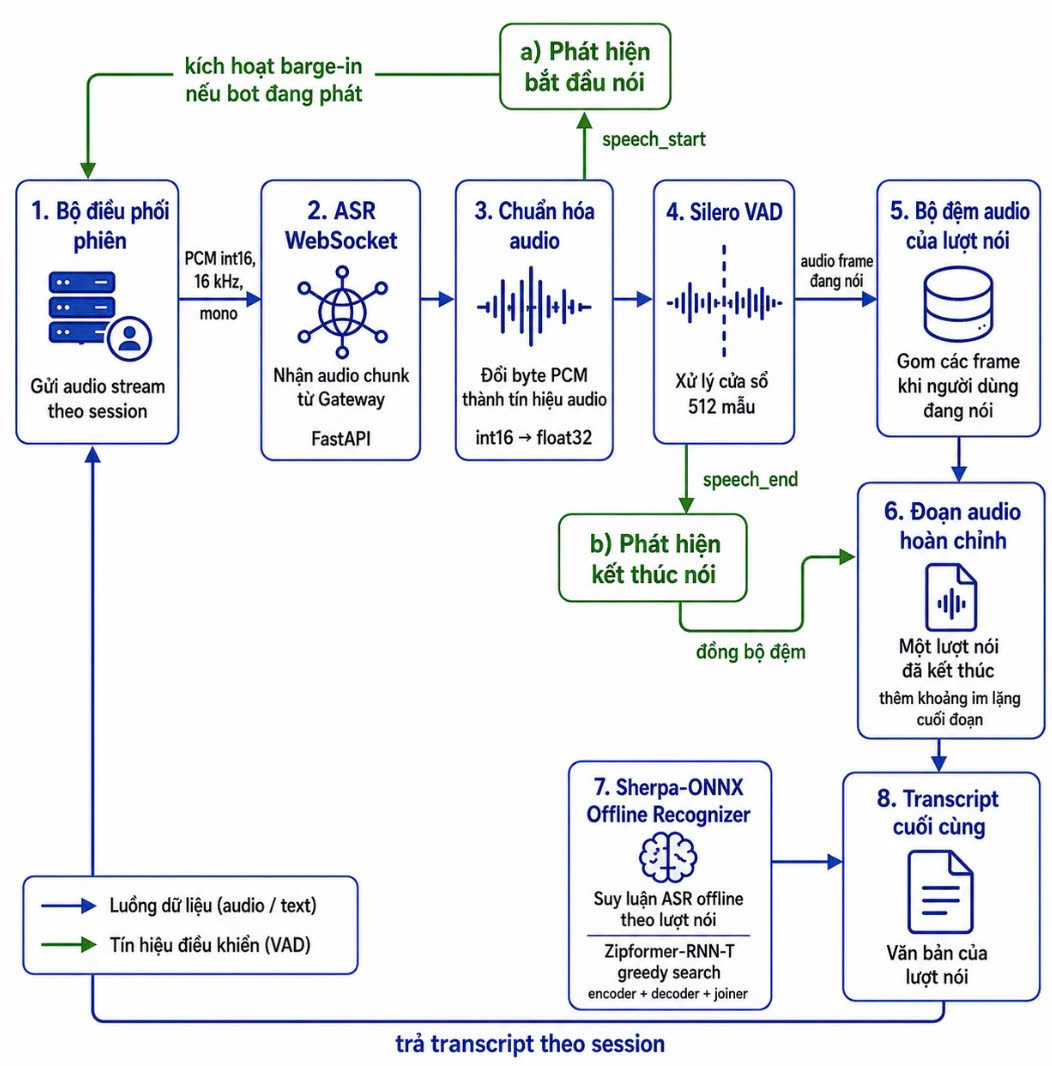
\includegraphics[width=0.86\textwidth]{report_figures/chapter4_asr_pipeline.png}
    \caption{Luồng xử lý trong mô-đun nhận dạng tiếng nói}
    \label{fig:chapter4-asr-pipeline}
\end{figure}

Hình~\ref{fig:chapter4-asr-pipeline} minh họa luồng xử lý cụ thể bên trong mô-đun nhận dạng tiếng nói. Điểm quan trọng của thiết kế này là audio được gửi liên tục để phát hiện ranh giới lượt nói, nhưng kết quả nhận dạng cuối cùng chỉ được tạo sau khi hệ thống xác định người dùng đã kết thúc lượt nói.

Silero VAD xử lý audio theo các cửa sổ 512 mẫu, tương ứng khoảng 32~ms ở tần số 16~kHz. Mỗi phiên hội thoại có trạng thái VAD riêng để phân biệt vùng im lặng, vùng đang nói và thời điểm kết thúc lượt nói. Khi VAD phát hiện điểm bắt đầu tiếng nói, mô-đun phát sự kiện \textit{speech\_start} về bộ điều phối phiên. Sự kiện này được dùng như tín hiệu điều khiển để kích hoạt barge-in nếu hệ thống đang phát phản hồi cũ. Nhờ vậy, phản hồi đang phát có thể được hủy sớm thay vì phải chờ người dùng nói xong.

Trong giai đoạn người dùng đang nói, các frame audio được ghi vào bộ đệm của lượt nói hiện tại. Bộ đệm này chỉ chứa audio thuộc cùng một lượt nói và cùng một session, giúp tránh trộn dữ liệu giữa các lượt hội thoại khác nhau. Khi VAD phát hiện \textit{speech\_end} sau một khoảng im lặng đủ dài, bộ đệm được đóng lại và tạo thành một đoạn audio hoàn chỉnh. Trước khi đưa đoạn audio này vào mô hình nhận dạng, hệ thống bổ sung một khoảng im lặng ngắn ở cuối đoạn để giúp mô hình xử lý hết các frame cuối.

Đoạn audio hoàn chỉnh được đưa vào Sherpa-ONNX OfflineRecognizer. Recognizer sử dụng checkpoint Zipformer--RNN-T tiếng Việt, trong đó mô hình transducer gồm các thành phần encoder, decoder và joiner. Cấu hình suy luận dùng tần số lấy mẫu 16~kHz, đặc trưng âm học 80 chiều và phương pháp giải mã greedy search. Đầu ra của bước này là transcript cuối cùng của lượt nói, được trả lại bộ điều phối phiên để chuyển tiếp sang mô-đun xử lý hội thoại.

Cách tổ chức trên phù hợp với mục tiêu của đồ án vì nó tách rõ hai nhiệm vụ: phát hiện ranh giới lượt nói theo thời gian thực và nhận dạng nội dung của lượt nói đã hoàn chỉnh. Thiết kế này không phải là nhận dạng từng token trong lúc người dùng vẫn đang nói, nhưng vẫn cho phép hệ thống phản ứng nhanh với tín hiệu bắt đầu nói để hỗ trợ barge-in, đồng thời giữ pipeline nhận dạng ổn định hơn trong điều kiện demo.


\subsection{Mô-đun xử lý hội thoại}

Mô-đun xử lý hội thoại là thành phần tiếp nhận transcript cuối cùng từ bộ điều phối phiên và tạo ra luồng văn bản phản hồi để chuyển tiếp sang TTS. Thành phần này được xây dựng bằng FastAPI và cung cấp giao diện \textit{/think/stream}. Kết quả trả về theo định dạng NDJSON streaming, trong đó mỗi dòng là một JSON chunk chứa phần văn bản mới sinh ra, trạng thái kết thúc, thông tin timing, trạng thái cache hoặc các metadata liên quan. Cách trả kết quả theo luồng giúp Gateway có thể bắt đầu gom text segment cho TTS ngay khi mô hình ngôn ngữ sinh được phần đầu của câu trả lời, thay vì chờ toàn bộ câu trả lời hoàn tất.

Đầu vào của mô-đun gồm bốn nhóm thông tin: câu hỏi hiện tại, mã phiên, lịch sử hội thoại gần nhất và bản tóm tắt phiên. Câu hỏi hiện tại là transcript cuối cùng do mô-đun nhận dạng tiếng nói trả về. Mã phiên được dùng để ghi log, gắn metadata và tránh trộn dữ liệu giữa các hội thoại. Lịch sử gần nhất và bản tóm tắt phiên được Gateway đọc từ bộ nhớ phiên rồi gửi kèm request, giúp mô hình xử lý được các câu hỏi nối tiếp như ``vậy trẻ em thì sao'' hoặc ``còn phụ nữ mang thai thì thế nào''.

\begin{figure}[H]
    \centering
    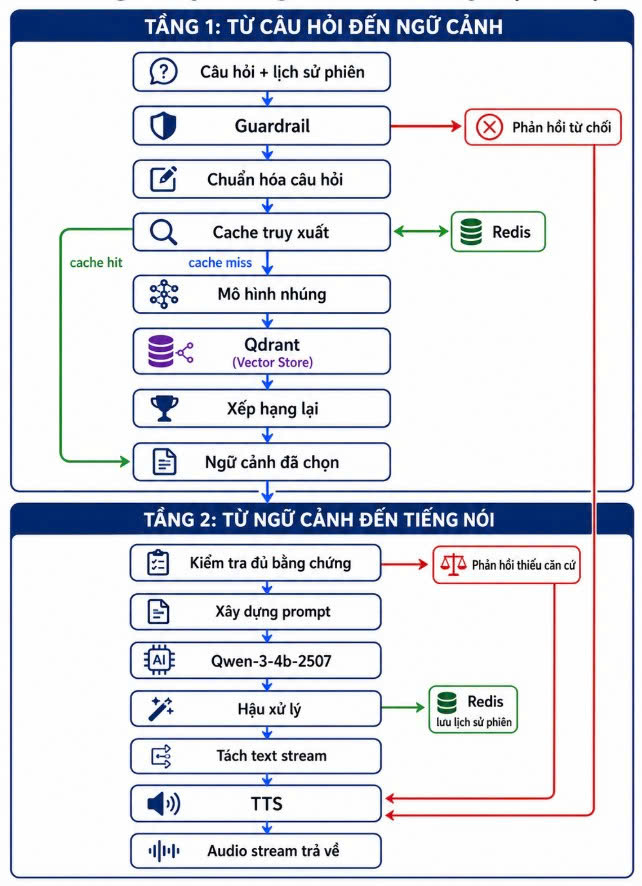
\includegraphics[width=0.78\textwidth]{report_figures/chapter4_dialogue_pipeline.jpg}
    \caption{Luồng xử lý trong mô-đun xử lý hội thoại}
    \label{fig:chapter4-dialogue-pipeline}
\end{figure}

Hình~\ref{fig:chapter4-dialogue-pipeline} trình bày luồng xử lý chi tiết của mô-đun xử lý hội thoại trong quá trình triển khai. Hình này làm rõ ba điểm chính: hệ thống kiểm tra phạm vi trước khi truy xuất, cache chỉ tái sử dụng ngữ cảnh truy xuất thay vì lưu câu trả lời cuối cùng, và mô hình ngôn ngữ chỉ được gọi khi câu hỏi hợp lệ và có đủ bằng chứng từ kho tri thức.

Bước đầu tiên trong luồng xử lý là guardrail đầu vào dựa trên luật. Hệ thống kiểm tra bốn nhóm trường hợp chính: câu hỏi rỗng hoặc không nghe rõ, dấu hiệu khẩn cấp y tế, yêu cầu chẩn đoán hoặc điều chỉnh thuốc, và câu hỏi nằm ngoài phạm vi dinh dưỡng. Các mẫu khẩn cấp bao gồm những cụm như khó thở, đau ngực, ngất, co giật, đột quỵ hoặc nôn ra máu. Các mẫu quyết định lâm sàng bao gồm kê đơn, hỏi liều thuốc, tăng giảm liều, ngừng thuốc hoặc yêu cầu chẩn đoán. Nếu guardrail được kích hoạt, mô-đun trả ngay một phản hồi cố định theo hướng từ chối mềm hoặc khuyến nghị gặp cơ sở y tế phù hợp. Khi đó hệ thống không thực hiện truy xuất, không gọi mô hình ngôn ngữ và không tiêu tốn thêm tài nguyên cho RAG.

Nếu câu hỏi hợp lệ, mô-đun thực hiện chuẩn hóa truy vấn bằng từ điển dinh dưỡng. Mục tiêu của bước này là giảm ảnh hưởng của cách nói tự nhiên sau ASR và tăng khả năng khớp với tài liệu trong kho tri thức. Ví dụ, ``tiểu đường'' được chuẩn hóa thành ``đái tháo đường'', ``bà bầu'' thành ``phụ nữ mang thai'', ``omega 3'' thành ``axit béo omega-3'', ``canxi'' thành ``canxi calcium'', và ``protein'' thành ``protein chất đạm''. Đây là bước đơn giản nhưng có tác dụng thực tế trong hệ thống tiếng Việt, vì người dùng thường dùng từ thông dụng trong khi tài liệu dinh dưỡng có thể dùng thuật ngữ chuyên môn hơn.

Sau chuẩn hóa, hệ thống đi vào tầng cache truy xuất. Tầng thứ nhất là cache truy xuất chính xác trong Redis. Khóa cache được tạo bằng cách băm các thông tin quyết định kết quả truy xuất, gồm câu hỏi sau chuẩn hóa, tên mô hình nhúng, tên mô hình xếp hạng lại, số đoạn ứng viên ban đầu, số đoạn cuối cùng, trạng thái bật HyDE và phiên bản corpus. Với cấu hình hiện tại, cache này có thời gian sống mặc định 86400 giây. Nếu cache khớp, hệ thống tái sử dụng danh sách tài liệu đã được xếp hạng lại, bỏ qua các bước mã hóa câu hỏi, tìm kiếm vector và chạy mô hình xếp hạng lại.

Nếu cache truy xuất chính xác không khớp, hệ thống kiểm tra cache truy xuất ngữ nghĩa. Câu hỏi được mã hóa thành vector và truy vấn trong một collection cache riêng của Qdrant. Cache ngữ nghĩa không chỉ dựa vào độ tương đồng vector, mà còn lọc theo chữ ký ngữ nghĩa gồm nhóm đối tượng, tình trạng và ý định hỏi. Ngoài ra, cache còn phải khớp phiên bản corpus, mô hình nhúng, mô hình xếp hạng lại, số lượng đoạn ứng viên và số lượng đoạn cuối cùng. Ngưỡng tương đồng mặc định là 0.90 và thời gian sống mặc định là 604800 giây. Cơ chế này giúp tái sử dụng ngữ cảnh cho các câu hỏi gần nghĩa, nhưng hạn chế dùng nhầm kết quả cho các câu hỏi có bề mặt giống nhau nhưng đối tượng hoặc mục đích khác nhau.

Khi không có cache phù hợp, hệ thống thực hiện truy xuất thật trên kho tri thức. Câu hỏi hoặc đoạn HyDE, nếu cấu hình HyDE được bật, được mã hóa bằng mô hình \textit{AITeamVN/Vietnamese\_Embedding} \cite{vietembedding}. Vector câu hỏi được chuẩn hóa trước khi truy vấn Qdrant \cite{qdrant}. Hệ thống lấy 15 đoạn văn bản ứng viên từ collection \textit{nutrition\_articles}. Mỗi kết quả truy xuất gồm nội dung đoạn văn bản và metadata như tiêu đề, nguồn, địa chỉ bài viết và điểm tương đồng vector. Nếu bước mã hóa quá 30 giây, hệ thống coi truy xuất không thành công để tránh một request treo làm nghẽn pipeline.

Các đoạn ứng viên sau đó được đưa vào mô hình xếp hạng lại \textit{thanhtantran/Vietnamese\_Reranker} \cite{vietreranker}. Mô hình này nhận từng cặp câu hỏi--đoạn văn bản và trả điểm phù hợp cho từng cặp. Hệ thống sắp xếp các đoạn theo điểm xếp hạng lại và chọn 5 đoạn tốt nhất để đưa vào prompt. Bước xếp hạng lại cũng có timeout 30 giây; nếu timeout, hệ thống dùng lại thứ tự theo điểm truy xuất vector và lấy các đoạn đầu tiên. Các bước mã hóa và xếp hạng lại dùng chung semaphore để giới hạn số tác vụ GPU chạy đồng thời, tránh nhiều request cùng lúc làm quá tải bộ nhớ hoặc làm tăng độ trễ đột biến.

Sau khi có các đoạn ngữ cảnh, mô-đun kiểm tra mức đủ tối thiểu của bằng chứng. Điều kiện hiện thực gồm ít nhất một đoạn tài liệu được truy xuất và tổng số ký tự ngữ cảnh đạt tối thiểu 120 ký tự. Nếu không thỏa điều kiện này, hệ thống trả về một phản hồi thận trọng, nói rằng chưa có đủ tài liệu dinh dưỡng đáng tin cậy để trả lời chính xác và gợi ý người dùng đặt lại câu hỏi cụ thể hơn. Nhánh này giúp hạn chế việc mô hình ngôn ngữ tự suy diễn khi kho tri thức không cung cấp đủ căn cứ.

Với ngữ cảnh đủ điều kiện, nội dung truy xuất được làm sạch trước khi đưa vào prompt. Hệ thống loại các dòng có dấu hiệu chèn lệnh vào ngữ cảnh như yêu cầu bỏ qua chỉ dẫn trước đó, nhắc tới system prompt, developer message hoặc yêu cầu đóng vai. Các URL và ký hiệu nguồn không cần thiết cũng được loại bỏ để câu trả lời cuối cùng phù hợp hơn với kênh tiếng nói. Sau đó, prompt được xây dựng từ các thành phần: chỉ dẫn hệ thống, hai ví dụ hỏi đáp mẫu, năm đoạn tài liệu dinh dưỡng đã chọn, bản tóm tắt hội thoại, lịch sử gần nhất và câu hỏi hiện tại. Chỉ dẫn hệ thống yêu cầu câu trả lời ngắn gọn, dễ nghe, dựa trên tài liệu, không nhắc tên nguồn hoặc URL, không chẩn đoán, không kê đơn và không điều chỉnh thuốc.

Mô hình ngôn ngữ được sử dụng ở bước sinh là Qwen-3-4b-2507. Mô-đun gọi mô hình theo chế độ streaming, nhận từng phần văn bản được sinh ra và ghi nhận thời gian tới chunk đầu tiên nếu backend trả metadata tương ứng. Các token đầu ra không được chuyển thẳng từng mảnh nhỏ về Gateway, mà được đưa qua bộ gom đoạn. Bộ gom đoạn tích lũy văn bản tới ngưỡng tối thiểu, ưu tiên cắt tại dấu kết thúc câu; nếu văn bản quá dài mà chưa có dấu câu phù hợp, hệ thống cắt tại khoảng trắng gần nhất. Cấu hình mặc định của mô-đun xử lý hội thoại dùng ngưỡng tối thiểu 40 ký tự. Cách gom đoạn này giúp giảm số chunk quá nhỏ, đồng thời vẫn giữ được khả năng bắt đầu TTS sớm.

Trong quá trình streaming, mỗi đoạn văn bản đầu ra được làm sạch để loại liên kết, markdown link và khoảng trắng thừa. Mô-đun cũng tích lũy toàn bộ văn bản đã phát ra để kiểm tra an toàn đầu ra sau khi sinh xong. Nếu câu trả lời thiếu câu khuyến nghị gặp bác sĩ dinh dưỡng, hệ thống bổ sung câu này ở cuối. Nếu phát hiện các mẫu không an toàn như ngừng thuốc, tăng liều, giảm liều hoặc khẳng định chắc chắn chữa khỏi, metadata đầu ra sẽ ghi nhận dấu hiệu này để phục vụ debug và đánh giá. Chunk cuối cùng của luồng không chứa thêm văn bản, mà chứa trạng thái kết thúc, các đoạn ngữ cảnh đã dùng, thông tin cache, đánh giá đủ bằng chứng và tổng thời gian xử lý.

Như vậy, mô-đun xử lý hội thoại không chỉ gọi mô hình ngôn ngữ để sinh câu trả lời, mà thực hiện một chuỗi bước kiểm soát trước và sau sinh. Guardrail quyết định câu hỏi có được đưa vào RAG hay không; cache giúp giảm lặp lại các bước truy xuất tốn thời gian; mô hình nhúng và Qdrant tạo tập ứng viên; mô hình xếp hạng lại chọn ngữ cảnh hẹp hơn; kiểm tra bằng chứng quyết định có đủ căn cứ để sinh hay không; cuối cùng, Qwen-3-4b-2507 sinh câu trả lời theo luồng để Gateway có thể chuyển dần sang TTS.

\subsection{Mô-đun TTS}

Mô-đun TTS là thành phần cuối của pipeline tiếng nói, nhận các text segment từ Gateway và chuyển thành audio stream trả về trình duyệt. Thành phần này được xây dựng bằng FastAPI và bọc VieNeu-TTS thông qua lớp tổng hợp tiếng nói riêng. Trong luồng chính, Gateway gọi giao diện streaming của TTS thay vì yêu cầu trả về một file âm thanh hoàn chỉnh. Đầu ra của mô-đun là các byte PCM int16, một kênh, tần số 24~kHz; các byte này được Gateway chuyển tiếp về giao diện dưới dạng binary frame để phát nối tiếp.

\begin{figure}[H]
    \centering
    \makebox[\textwidth][c]{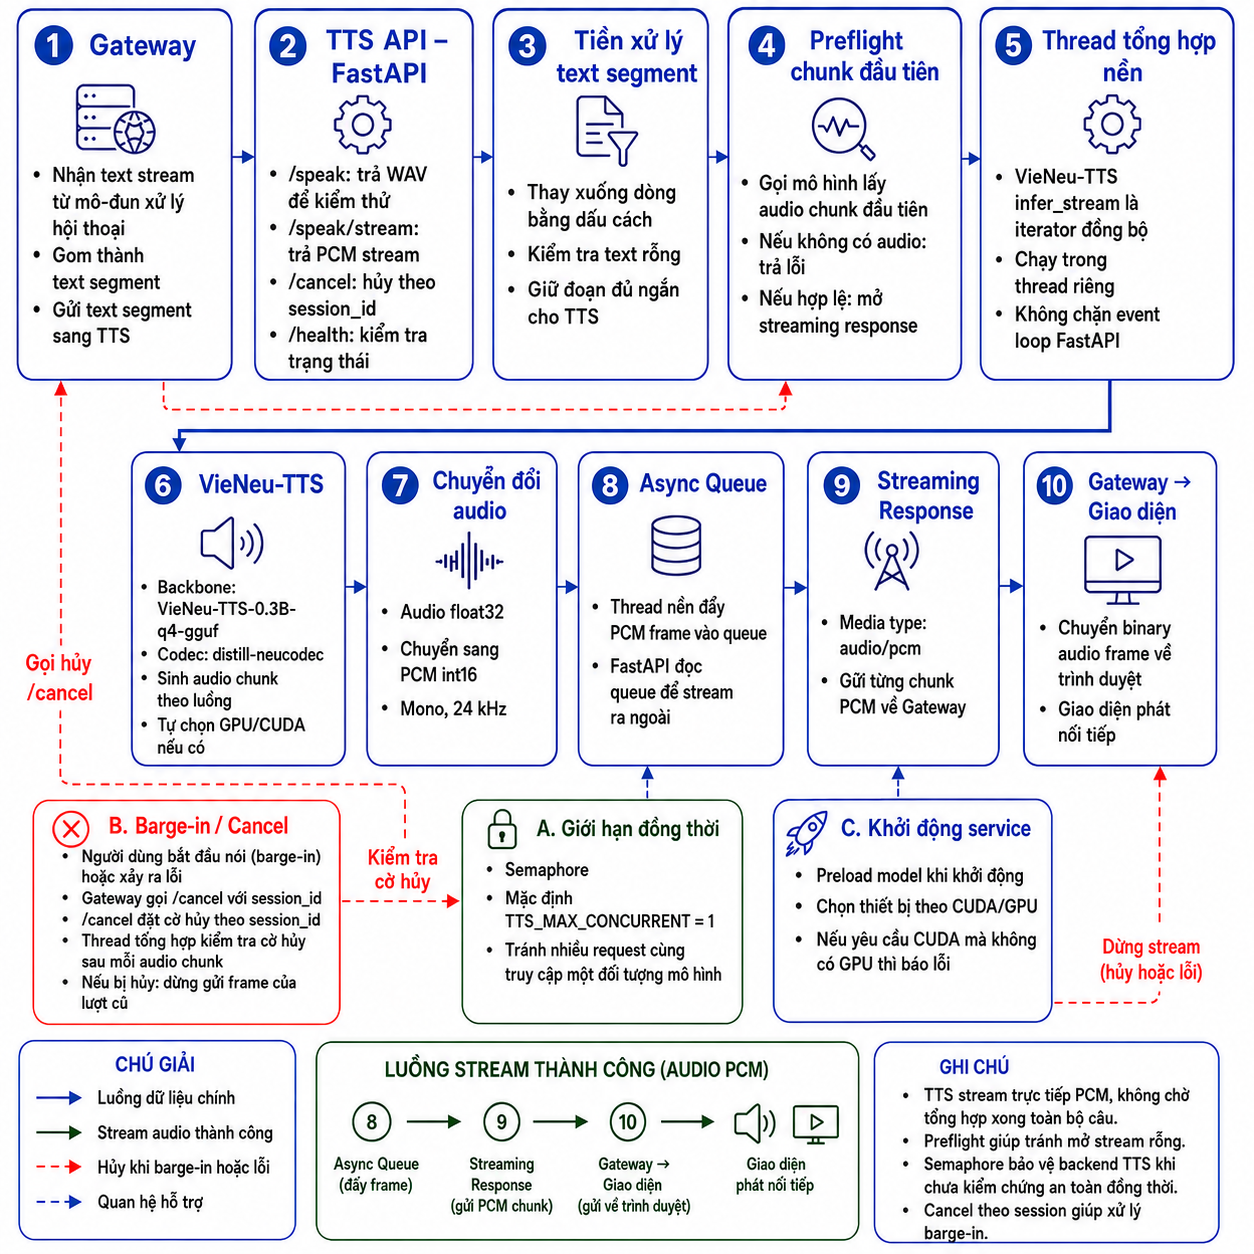
\includegraphics[width=0.98\textwidth]{report_figures/chapter4_tts_module.png}}
    \caption{Luồng xử lý trong mô-đun TTS}
    \label{fig:chapter4-tts-module}
\end{figure}

Hình~\ref{fig:chapter4-tts-module} mô tả luồng xử lý bên trong mô-đun TTS khi nhận một text segment từ Gateway. Điểm chính của thiết kế là tách quá trình tổng hợp đồng bộ của VieNeu-TTS khỏi event loop của FastAPI bằng thread nền và hàng đợi bất đồng bộ. Nhờ đó, service có thể stream từng frame âm thanh ra ngoài, đồng thời vẫn hỗ trợ hủy tổng hợp theo session khi xảy ra barge-in.

Mô-đun cung cấp ba nhóm giao diện chính. Thứ nhất là giao diện kiểm tra trạng thái, trả về tình trạng service, trạng thái nạp mô hình và kết nối tới Redis nếu được bật trong cấu hình. Thứ hai là giao diện tổng hợp đầy đủ, nhận văn bản và trả về file WAV cùng các header đo đạc như thời gian tới byte đầu tiên, hệ số thời gian thực và thời lượng âm thanh. Giao diện này chủ yếu phục vụ kiểm thử hoặc đo riêng mô-đun TTS. Thứ ba là giao diện streaming, nhận văn bản và trả dần các chunk PCM ngay khi mô hình sinh được âm thanh. Pipeline hội thoại sử dụng giao diện streaming vì mục tiêu chính là giảm thời gian chờ trước khi người dùng nghe được âm thanh đầu tiên.

Khi khởi động, lớp tổng hợp tiếng nói nạp VieNeu-TTS với hai thành phần: backbone sinh token tiếng nói và codec âm thanh. Backbone mặc định trong cấu hình là \textit{pnnbao-ump/VieNeu-TTS-0.3B-q4-gguf}, còn codec là \textit{neuphonic/distill-neucodec}. Mô-đun tự chọn thiết bị dựa trên khả năng CUDA của môi trường: nếu có GPU, backbone được đặt ở chế độ GPU và codec dùng CUDA; nếu không, hệ thống có thể chạy ở CPU cho mục đích kiểm thử chức năng. Khi biến cấu hình yêu cầu CUDA được bật, service sẽ báo lỗi nếu container không có GPU phù hợp. Cấu hình mặc định nạp mô hình ngay trong giai đoạn khởi động service để tránh độ trễ lớn ở request đầu tiên.

Trước khi đưa văn bản vào mô hình, TTS thực hiện bước tiền xử lý đơn giản ở mức service. Các ký tự xuống dòng do mô hình ngôn ngữ sinh ra được thay bằng dấu cách để tránh việc TTS đọc ngắt bất thường giữa câu. Trong pipeline chính, việc chia văn bản thành text segment đã được Gateway thực hiện trước đó dựa trên luồng sinh của mô hình ngôn ngữ. Vì vậy TTS thường nhận từng đoạn đủ ngắn để tổng hợp ngay. Bên trong VieNeu-TTS vẫn có giới hạn độ dài tối đa cho mỗi lần suy luận; nếu một đoạn quá dài, thư viện có thể tiếp tục chia nhỏ theo cấu hình nội bộ.

Điểm quan trọng của hiện thực TTS là chuyển một iterator đồng bộ thành stream bất đồng bộ. API streaming của VieNeu-TTS trả về từng audio chunk thông qua vòng lặp đồng bộ. Nếu gọi trực tiếp trong luồng xử lý HTTP bất đồng bộ, service sẽ dễ chặn event loop của FastAPI. Để tránh điều này, TTS tạo một thread nền cho tác vụ tổng hợp. Thread này đọc từng frame âm thanh từ VieNeu-TTS, chuyển dữ liệu float32 sang PCM int16 và đẩy vào một hàng đợi bất đồng bộ. Phía FastAPI đọc hàng đợi này và stream từng chunk ra ngoài. Nhờ cơ chế này, service có thể gửi chunk âm thanh đầu tiên ngay khi mô hình tạo được frame đầu tiên, thay vì phải chờ toàn bộ đoạn văn bản được tổng hợp xong.

Trong giao diện streaming, TTS thực hiện một bước kiểm tra trước khi mở luồng phản hồi. Service gọi mô hình để lấy chunk âm thanh đầu tiên. Nếu mô hình không trả audio hoặc phát sinh lỗi, service trả lỗi ngay cho Gateway thay vì mở một stream rỗng khiến Gateway chờ vô hạn. Nếu chunk đầu tiên hợp lệ, service bắt đầu trả \textit{StreamingResponse}; chunk đầu tiên được gửi trước, các chunk tiếp theo được gửi khi thread nền tiếp tục nhận được frame mới từ mô hình.

Để tránh nhiều request đồng thời cùng truy cập trạng thái mô hình trong một tiến trình, mô-đun giới hạn số tác vụ tổng hợp chạy song song bằng semaphore. Cấu hình mặc định của biến \textit{TTS\_MAX\_CONCURRENT} là 1, tức tại một thời điểm chỉ có một tác vụ tổng hợp thực sự chạy trong worker TTS. Đây là lựa chọn thận trọng vì backend hiện tại chưa được coi là an toàn khi nhiều suy luận cùng sử dụng chung đối tượng mô hình. Khi cần tăng thông lượng, hướng phù hợp hơn là chạy nhiều instance TTS độc lập hoặc kiểm thử lại độ an toàn đồng thời của backend trước khi tăng giới hạn này.

Mô-đun TTS cũng hỗ trợ hủy tổng hợp theo session để phục vụ barge-in. Với mỗi session đang tổng hợp, lớp tổng hợp tiếng nói tạo một cờ hủy riêng. Khi Gateway phát hiện người dùng bắt đầu nói trong lúc hệ thống đang phát phản hồi, Gateway gọi giao diện hủy của TTS với session tương ứng. Nếu vòng lặp tổng hợp đang chạy, nó kiểm tra cờ hủy ở mỗi audio chunk; khi cờ được bật, vòng lặp dừng và không tiếp tục gửi frame của lượt cũ. Cơ chế này giúp hạn chế việc âm thanh cũ vẫn tiếp tục phát sau khi người dùng đã bắt đầu lượt nói mới.

Như vậy, mô-đun TTS không chỉ thực hiện chuyển văn bản thành âm thanh, mà còn đảm nhiệm các yêu cầu vận hành quan trọng của hệ thống hội thoại: nạp mô hình theo cấu hình phần cứng, stream PCM trực tiếp, không chặn event loop, kiểm tra chunk đầu tiên trước khi mở stream, giới hạn đồng thời để bảo vệ backend và hủy tác vụ theo session khi xảy ra barge-in.

\subsection{Cơ sở dữ liệu, cache và dữ liệu phiên}

Hệ thống sử dụng hai loại lưu trữ chính. Qdrant giữ kho tri thức dạng vector, còn Redis giữ trạng thái phiên và cache truy xuất. Cách tách này phản ánh hai nhu cầu khác nhau: Qdrant phục vụ tìm kiếm ngữ nghĩa trên tập tài liệu lớn, trong khi Redis phục vụ các thao tác đọc ghi nhỏ, cần độ trễ thấp và có thời gian sống ngắn theo phiên hoặc theo cấu hình cache.

Hình~\ref{fig:chapter4-storage-cache-session} minh họa cách các thành phần lưu trữ tham gia vào luồng xử lý. Redis phục vụ hai nhóm dữ liệu có vòng đời ngắn là bộ nhớ phiên và cache truy xuất chính xác. Qdrant phục vụ hai nhóm dữ liệu dạng vector là kho tri thức chính và cache truy xuất ngữ nghĩa. Snapshot Qdrant được dùng ở thời điểm triển khai hoặc khởi động để khôi phục nhanh kho tri thức, không phải một bước chạy trong từng lượt hỏi đáp.

\begin{figure}[H]
    \centering
    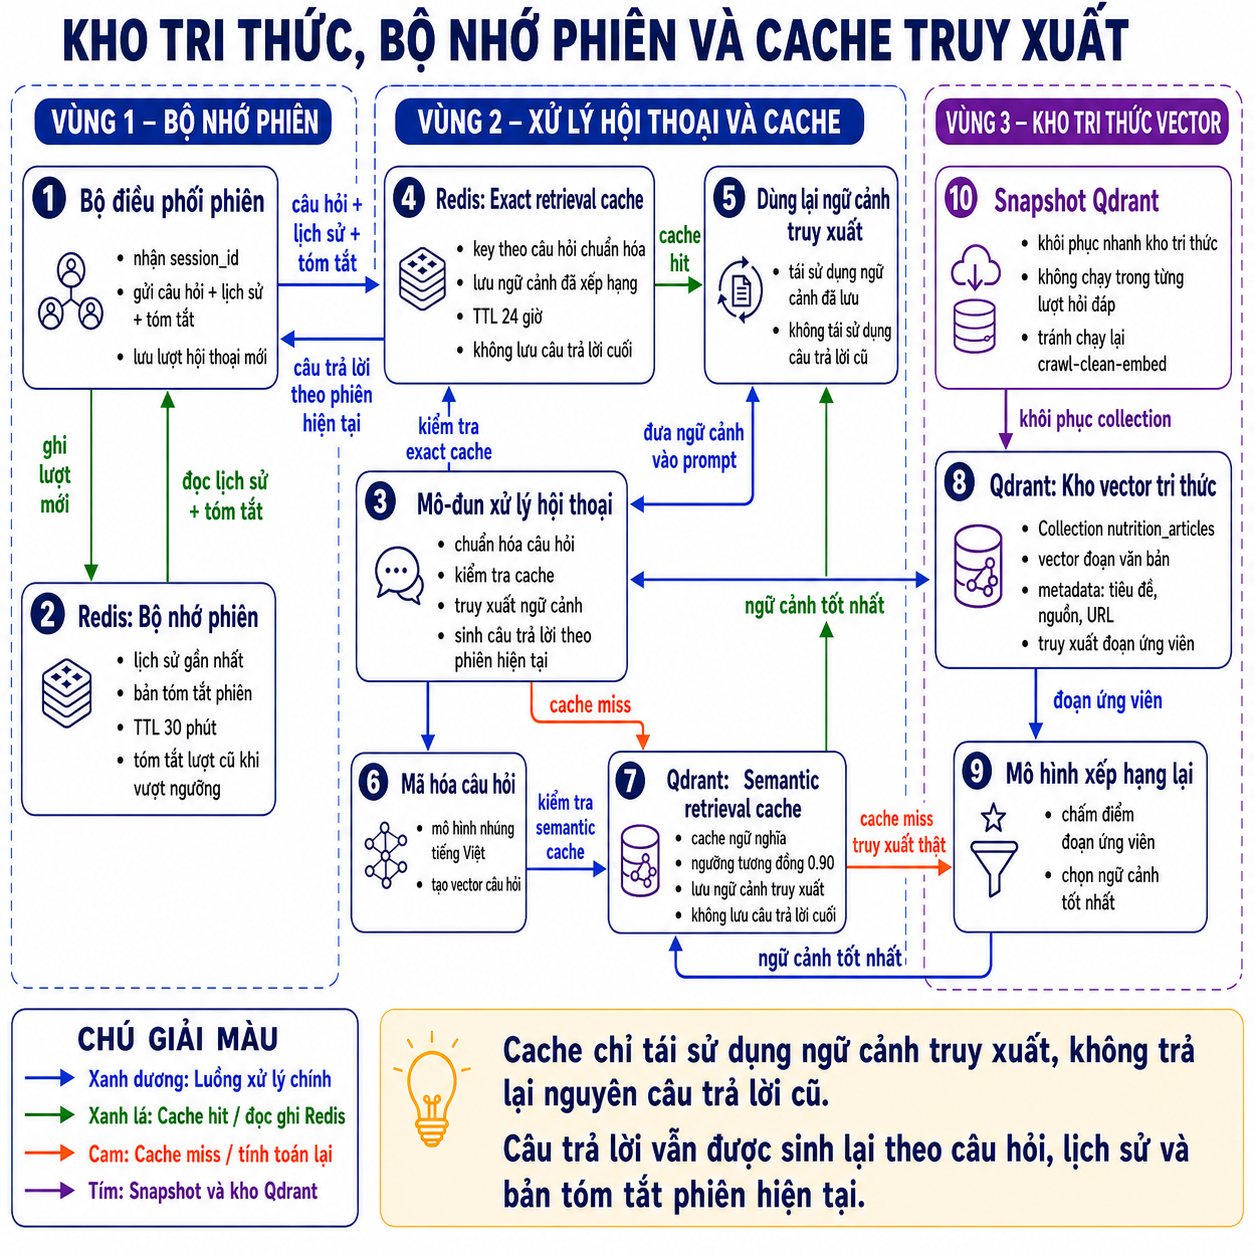
\includegraphics[width=0.9\textwidth]{report_figures/chapter4_storage_cache_session.png}
    \caption{Cơ sở dữ liệu, cache và dữ liệu phiên trong hệ thống}
    \label{fig:chapter4-storage-cache-session}
\end{figure}

Trong Qdrant, mỗi điểm dữ liệu biểu diễn một đoạn văn bản trong kho tri thức dinh dưỡng. Redis phục vụ hai nhóm dữ liệu có vòng đời ngắn là bộ nhớ phiên và cache truy xuất chính xác. Qdrant phục vụ hai nhóm dữ liệu dạng vector là kho tri thức chính và cache truy xuất ngữ nghĩa. Snapshot Qdrant được dùng ở thời điểm triển khai hoặc khởi động để khôi phục nhanh kho tri thức, không phải một bước chạy trong từng lượt hỏi đáp.

Trong Qdrant, mỗi điểm dữ liệu biểu diễn một đoạn văn bản trong kho tri thức dinh dưỡng. Điểm dữ liệu gồm vector nhúng và phần dữ liệu đi kèm như tiêu đề bài viết, nguồn, địa chỉ bài viết, nội dung đoạn văn bản và các thông tin phục vụ truy vết. Collection chính của hệ thống là kho các đoạn văn bản dinh dưỡng đã được mã hóa. Khi mô-đun xử lý hội thoại nhận câu hỏi, vector của câu hỏi sau chuẩn hóa được dùng để truy vấn collection này và lấy ra các đoạn ứng viên. Các đoạn ứng viên sau đó được mô hình xếp hạng lại đánh giá thêm trước khi chọn làm ngữ cảnh cho mô hình ngôn ngữ.

Qdrant cũng được dùng để khôi phục nhanh kho tri thức khi triển khai. Cấu hình hệ thống cho phép chỉ định đường dẫn snapshot của collection. Khi khởi động, nếu collection đã có dữ liệu thì bước khôi phục được bỏ qua; nếu collection chưa có dữ liệu hoặc cấu hình yêu cầu khôi phục lại, hệ thống nạp snapshot vào Qdrant trước khi phục vụ truy vấn. Cơ chế này giúp môi trường demo hoặc môi trường máy chủ mới không phải chạy lại toàn bộ pipeline thu thập, làm sạch, phân đoạn và mã hóa dữ liệu.

Redis được sử dụng trước hết cho bộ nhớ phiên hội thoại. Với mỗi session, hệ thống lưu hai nhóm thông tin: danh sách các lượt hội thoại gần nhất và bản tóm tắt tích lũy của các lượt cũ hơn. Cấu hình mặc định giữ tối đa ba lượt gần nhất ở dạng nguyên văn. Khi số lượt vượt quá ngưỡng này, các lượt cũ được tách ra để tóm tắt bất đồng bộ thông qua mô-đun xử lý hội thoại, còn Redis chỉ giữ lại hai lượt mới nhất cùng bản tóm tắt đã cập nhật. Các khóa phiên có thời gian sống mặc định 30 phút, giúp trạng thái hội thoại tự hết hạn nếu người dùng không tiếp tục tương tác.

Việc cập nhật lịch sử phiên được thực hiện theo hướng nguyên tử. Khi thêm một lượt mới, hệ thống đọc danh sách lượt hiện có, nối lượt mới, cắt bớt các lượt cũ nếu vượt ngưỡng và ghi lại vào Redis trong cùng một thao tác. Nhờ vậy, lịch sử của một session không bị ghi đè sai thứ tự khi nhiều thao tác đọc ghi xảy ra gần nhau. Phần tóm tắt được cập nhật bằng một tác vụ nền, nên việc nén lịch sử không chặn luồng phản hồi hiện tại của người dùng.

Ngoài bộ nhớ phiên, Redis còn lưu cache truy xuất chính xác. Khóa cache được tạo từ câu hỏi sau chuẩn hóa, tên mô hình nhúng, tên mô hình xếp hạng lại, số đoạn ứng viên ban đầu, số đoạn cuối cùng, trạng thái dùng HyDE và phiên bản corpus. Giá trị cache là danh sách các đoạn văn bản đã được truy xuất và xếp hạng lại, kèm thời gian tính toán ước lượng. Thời gian sống mặc định của cache truy xuất chính xác là 86400 giây. Khi cache khớp, hệ thống bỏ qua bước mã hóa câu hỏi, truy vấn Qdrant và xếp hạng lại, sau đó dùng lại ngữ cảnh truy xuất để đi tiếp tới bước kiểm tra mức đủ bằng chứng.

Để hỗ trợ các câu hỏi gần nghĩa, hệ thống còn có cache truy xuất ngữ nghĩa. Cache này được lưu trong một collection riêng của Qdrant. Sau khi câu hỏi được mã hóa thành vector, hệ thống truy vấn collection cache với ngưỡng tương đồng mặc định 0.90. Kết quả cache chỉ được chấp nhận nếu đồng thời khớp chữ ký ngữ nghĩa của câu hỏi, phiên bản corpus, mô hình nhúng, mô hình xếp hạng lại và cấu hình số đoạn truy xuất. Chữ ký ngữ nghĩa tách câu hỏi theo nhóm đối tượng, tình trạng và ý định hỏi, giúp hạn chế việc dùng lại ngữ cảnh của một câu hỏi giống bề mặt nhưng khác đối tượng tư vấn.

Điểm quan trọng là cả cache chính xác và cache ngữ nghĩa đều chỉ lưu ngữ cảnh truy xuất, không lưu câu trả lời cuối cùng. Khi cache hit, hệ thống vẫn kiểm tra mức đủ bằng chứng, xây dựng prompt theo lịch sử phiên hiện tại và gọi mô hình ngôn ngữ để sinh câu trả lời mới. Cách này giữ được lợi ích giảm độ trễ của cache, nhưng vẫn tránh việc trả nguyên một câu trả lời cũ trong bối cảnh hội thoại đã thay đổi.

Về mặt vận hành, các cache cũng ghi lại thống kê như số lượt hit, miss, số lượt ghi, lỗi đọc ghi và thời gian ước lượng tiết kiệm được. Các thông tin này được dùng để kiểm tra hiệu quả cache khi chạy thử nghiệm. Nếu Redis không sẵn sàng và cấu hình không yêu cầu bắt buộc cache, hệ thống vẫn có thể tiếp tục phục vụ truy vấn ở chế độ không cache; khi đó độ trễ có thể tăng nhưng luồng hỏi đáp chính không bị dừng.

\section{Xây dựng hệ thống}

\subsection{Hiện thực luồng giao tiếp và điều phối phiên}

Luồng giao tiếp được hiện thực theo mô hình streaming hai chiều. Ở chiều vào, giao diện gửi các đoạn PCM 16~kHz tới Gateway. Gateway chuyển tiếp các đoạn này sang ASR qua một kết nối streaming riêng và tiếp tục nhận sự kiện từ ASR trong lúc audio vẫn đang đến. Điều này cho phép Gateway phản ứng ngay với tín hiệu bắt đầu nói, thay vì chỉ xử lý sau khi người dùng kết thúc toàn bộ lượt nói.

Ở chiều ra, mô-đun xử lý hội thoại sinh text stream, Gateway chia thành text segment và TTS trả audio stream. Gateway phát sự kiện bắt đầu audio trước chunk âm thanh đầu tiên để giao diện reset hàng đợi phát. Các chunk âm thanh được gửi về giao diện dưới dạng binary, còn transcript, text stream, lỗi và trạng thái được gửi bằng JSON. Việc tách binary audio và JSON event giúp giao diện xử lý hai loại dữ liệu theo hai đường rõ ràng.

Barge-in được hiện thực tại cả tầng giao diện và Gateway. Khi ASR gửi tín hiệu bắt đầu nói, Gateway hủy tác vụ đang sinh phản hồi và gọi TTS hủy theo session. Đồng thời, Gateway gửi sự kiện ngắt bot về giao diện để xóa phần audio cũ. Nếu tín hiệu bắt đầu nói bị bỏ lỡ nhưng transcript mới xuất hiện trong lúc phản hồi cũ vẫn đang chạy, Gateway vẫn thực hiện hủy như một cơ chế dự phòng.

\subsection{Hiện thực các mô-đun xử lý AI}

ASR được hiện thực theo hai chế độ. Chế độ thứ nhất nhận toàn bộ audio và trả transcript một lần, phù hợp cho kiểm thử hoặc gửi file audio. Chế độ thứ hai dùng WebSocket kết hợp VAD để xử lý audio stream từ phiên hội thoại. Trong demo tương tác thời gian thực, hệ thống sử dụng chế độ VAD để xác định lượt nói và chỉ gọi nhận dạng khi đoạn audio hoàn chỉnh.

Mô-đun xử lý hội thoại hiện thực pipeline RAG theo thứ tự: guardrail, mở rộng truy vấn, kiểm tra cache, truy xuất vector, xếp hạng lại, kiểm tra bằng chứng, xây dựng prompt và sinh câu trả lời. Các thông tin timing như thời gian mở rộng truy vấn, thời gian RAG, thời gian tới chunk đầu tiên của mô hình ngôn ngữ và tổng thời gian được trả kèm trong stream để phục vụ đo đạc ở Chương 5.

TTS được hiện thực theo hướng stream-first. Đường xử lý tổng hợp dạng đầy đủ vẫn tồn tại để trả WAV và các header đo thời gian, nhưng pipeline chính sử dụng luồng PCM trực tiếp. Với mỗi text segment, TTS thực hiện preflight để lấy chunk đầu tiên trước khi mở stream phản hồi; nếu mô hình không trả audio, hệ thống báo lỗi thay vì để Gateway chờ vô hạn.

\subsection{Đóng gói, cấu hình và kiểm thử chức năng}

Docker Compose được dùng để khởi động toàn bộ hệ thống bằng một cấu hình thống nhất. Mỗi thành phần có Dockerfile riêng để tách môi trường phụ thuộc. Gateway phụ thuộc vào Redis, ASR, mô-đun xử lý hội thoại và TTS; mô-đun xử lý hội thoại phụ thuộc vào Qdrant, bước khôi phục snapshot và Redis; TTS phụ thuộc vào Redis khi bật cache. Các healthcheck giúp phát hiện sớm tình trạng service chưa sẵn sàng.

Cấu hình GPU bổ sung vLLM để phục vụ Qwen-3-4b-2507 qua giao thức tương thích OpenAI API. Cấu hình này cũng dùng Dockerfile GPU cho ASR, mô-đun xử lý hội thoại và TTS. Các biến môi trường điều khiển mô hình nhúng, mô hình xếp hạng lại, ngưỡng VAD, số đoạn truy xuất, TTL cache, corpus version và chế độ yêu cầu CUDA. Nhờ vậy, cùng một codebase có thể chạy ở môi trường CPU để kiểm thử chức năng hoặc môi trường GPU để đo độ trễ.

Trong quá trình xây dựng, kiểm thử chức năng được chia thành hai mức. Mức thứ nhất là kiểm thử đơn vị cho các hàm có đầu vào và đầu ra xác định như mở rộng truy vấn, guardrail, kiểm tra ngữ cảnh, tạo khóa cache, phân đoạn văn bản và xây dựng prompt. Mức thứ hai là kiểm thử tích hợp theo luồng từ giao diện đến Gateway, ASR, mô-đun xử lý hội thoại, TTS và trả âm thanh về giao diện. Kiểm thử tích hợp tập trung vào việc dữ liệu đi đúng session, văn bản và âm thanh được truyền đúng thứ tự, lịch sử hội thoại được duy trì và phản hồi cũ được hủy khi xảy ra barge-in.

\begingroup
\small
\renewcommand{\arraystretch}{1.05}
\setlength{\LTleft}{\fill}
\setlength{\LTright}{\fill}
\begin{longtable}{|p{4.0cm}|p{8.5cm}|}
    \hline
    \textbf{Nhóm kiểm thử} & \textbf{Nội dung xác minh}                                                                                 \\
    \hline
    Mở rộng truy vấn       & Chuẩn hóa và bổ sung các cách diễn đạt tương đương trong chủ đề dinh dưỡng.                                \\
    \hline
    Guardrail an toàn      & Nhận biết một số câu hỏi ngoài phạm vi, tình huống khẩn cấp và yêu cầu liên quan đến chẩn đoán hoặc thuốc. \\
    \hline
    Kiểm soát RAG          & Kiểm tra mức đủ của ngữ cảnh và làm sạch nội dung trước khi đưa vào prompt.                                \\
    \hline
    Cache truy xuất        & Tính ổn định của khóa cache, chuẩn hóa câu hỏi và phân tách phiên bản kho tri thức.                        \\
    \hline
    Semantic cache         & Phân biệt nhóm người dùng, tình trạng và ý định khi tái sử dụng kết quả truy xuất gần nghĩa.               \\
    \hline
    Phân đoạn văn bản      & Tách văn bản theo dấu câu và ngưỡng độ dài trước khi gửi sang TTS.                                         \\
    \hline
    Xây dựng prompt        & Ghép chỉ dẫn, ngữ cảnh truy xuất, lịch sử hội thoại và câu hỏi theo đúng cấu trúc.                         \\
    \hline
    Luồng tích hợp         & Kiểm tra dữ liệu đúng session, thứ tự audio/text stream và hủy phản hồi khi barge-in.                      \\
    \hline
    \caption{Phạm vi kiểm thử chức năng trong quá trình xây dựng}
    \label{tab:unit-test-scope}
\end{longtable}
\endgroup

Kết quả của giai đoạn xây dựng là một hệ thống có thể khởi động bằng cấu hình thống nhất, kiểm tra trạng thái từng thành phần và thực hiện một lượt hỏi đáp bằng tiếng nói trên giao diện. Trong một lượt demo, người dùng đặt câu hỏi dinh dưỡng, hệ thống tạo transcript, truy xuất ngữ cảnh, sinh câu trả lời theo luồng và bắt đầu phát âm thanh trước khi toàn bộ văn bản được sinh xong. Các kết quả thực nghiệm về RAG, ASR, TTS và độ trễ được trình bày ở Chương 5.

\chapter{THỰC NGHIỆM VÀ ĐÁNH GIÁ}

\section{Xây dựng kho tri thức và tập dữ liệu}

Kho tri thức là nguồn ngữ cảnh bên ngoài được sử dụng để giới hạn quá trình sinh câu trả lời của mô hình ngôn ngữ. Do nội dung tư vấn dinh dưỡng có liên quan đến sức khỏe, việc xây dựng kho tri thức không chỉ nhằm tăng số lượng tài liệu có thể truy xuất mà còn phải kiểm soát nguồn, loại bỏ nội dung nhiễu và bảo toàn ngữ nghĩa khi phân đoạn. Quy trình được tổ chức thành năm bước chính: thu thập bài viết, chuẩn hóa cấu trúc dữ liệu, làm sạch nội dung, phân đoạn tài liệu và mã hóa các đoạn văn bản để lưu vào Qdrant.

Bên cạnh kho tri thức dùng cho truy xuất, đồ án sử dụng các tập dữ liệu đánh giá riêng cho từng nhóm thực nghiệm. Tập đánh giá RAG gồm các câu hỏi dinh dưỡng, câu trả lời tham chiếu và ngữ cảnh liên quan để đo chất lượng câu trả lời. Tập đánh giá ASR gồm audio tiếng Việt và transcript tham chiếu để tính lỗi nhận dạng và tốc độ xử lý. Tập đánh giá độ trễ gồm các lượt hỏi đáp được chạy qua hệ thống với nhiều cấu hình chia đoạn văn bản nhằm đo Time-to-First-Audio và tổng thời gian phản hồi. Việc tách dữ liệu xây dựng kho tri thức khỏi dữ liệu đánh giá giúp tránh nhầm lẫn giữa nguồn trả lời và nguồn dùng để đo chất lượng.

\subsection{Thu thập và tổ chức dữ liệu nguồn}

Trong phạm vi đồ án, tập dữ liệu được lựa chọn gồm 1060 bài viết về dinh dưỡng từ ba nguồn công khai có tính chuyên môn: Báo Sức khỏe và Đời sống, Viện Dinh dưỡng Quốc gia và Bệnh viện Đa khoa Quốc tế Thu Cúc. Các nguồn này cung cấp nội dung về dinh dưỡng theo lứa tuổi, chế độ ăn cho một số bệnh nền thường gặp, vitamin và khoáng chất, kiểm soát cân nặng, dinh dưỡng cho trẻ em, phụ nữ mang thai và người cao tuổi.

Pipeline thu thập trong mã nguồn cũng hỗ trợ xử lý các bài viết và nội dung hỏi đáp từ Vinmec. Tuy nhiên, số liệu 1060 bài được sử dụng trong phạm vi báo cáo này chỉ tính ba nguồn nêu trên. Việc phân biệt này giúp tránh nhầm lẫn giữa các nguồn mà công cụ thu thập có khả năng xử lý và tập dữ liệu thực tế được lựa chọn để xây dựng kho tri thức của đồ án.

Quá trình thu thập được điều chỉnh theo đặc điểm của từng trang web. Với trang có nội dung tải động và danh sách bài viết được mở rộng bằng thao tác cuộn hoặc nút xem thêm, trình duyệt tự động được sử dụng để thu thập liên kết và đọc phần nội dung đã được hiển thị. Với các trang tĩnh, hệ thống gửi yêu cầu HTTP và phân tích cấu trúc HTML để lấy tiêu đề, nội dung chính và chuyên mục. Các khối không thuộc nội dung bài viết như quảng cáo, nút chia sẻ, bài viết liên quan, bình luận và thành phần điều hướng được loại bỏ ngay trong bước trích xuất.

Mỗi bài viết được lưu thành một bản ghi có cấu trúc thống nhất gồm nguồn, địa chỉ bài viết, tiêu đề, nội dung, chuyên mục và thời điểm thu thập. Địa chỉ bài viết được sử dụng làm khóa kiểm tra trùng lặp. Trước khi ghi một bản ghi mới, chương trình kiểm tra danh sách địa chỉ đã thu thập để tránh lưu lại cùng một bài nhiều lần. Cơ chế này đồng thời cho phép tiếp tục quá trình thu thập sau khi bị gián đoạn mà không phải thực hiện lại từ đầu. Các bài không có tiêu đề, không xác định được vùng nội dung chính hoặc có nội dung quá ngắn bị loại bỏ. Cấu trúc một bản ghi trước khi phân đoạn được mô tả trong Bảng~\ref{tab:raw-document-schema}.

\begin{table}[H]
    \centering
    \begin{tabular}{|p{3.2cm}|p{10.2cm}|}
        \hline
        \textbf{Trường dữ liệu} & \textbf{Ý nghĩa}                                                          \\
        \hline
        Nguồn                   & Tên đơn vị hoặc trang web cung cấp bài viết.                              \\
        \hline
        Địa chỉ bài viết        & Định danh tài liệu, phục vụ loại bỏ trùng lặp và truy vết nguồn.          \\
        \hline
        Tiêu đề                 & Mô tả chủ đề chính của bài viết và bổ sung ngữ cảnh cho quá trình mã hóa. \\
        \hline
        Nội dung                & Phần văn bản chính được sử dụng để phân đoạn và xây dựng kho tri thức.    \\
        \hline
        Chuyên mục              & Nhóm nội dung của bài viết, hỗ trợ thống kê và lọc dữ liệu khi cần.       \\
        \hline
        Thời điểm thu thập      & Thông tin phục vụ quản lý phiên bản và cập nhật dữ liệu.                  \\
        \hline
    \end{tabular}
    \caption{Cấu trúc một bản ghi tài liệu trước khi phân đoạn}
    \label{tab:raw-document-schema}
\end{table}

\subsection{Làm sạch và chuẩn hóa văn bản}

Văn bản lấy trực tiếp từ trang web thường chứa các thành phần không có ích cho truy xuất như mục lục được sinh tự động, đường dẫn đứng riêng, dòng phân cách, thông tin đăng nhập, liên hệ, bản quyền, tên tác giả lặp lại hoặc phần tài liệu tham khảo ở cuối bài. Nếu giữ lại các nội dung này, mô hình embedding có thể biểu diễn cả phần nhiễu và làm giảm mức tương đồng giữa câu hỏi với đoạn văn bản thực sự liên quan.

Quá trình làm sạch trước hết chuẩn hóa các ký tự khoảng trắng đặc biệt, loại bỏ ký tự vô hình và rút gọn khoảng trắng hoặc dòng trống liên tiếp. Tiếp theo, chương trình nhận biết và loại bỏ các dòng chỉ chứa đường dẫn, dòng phân cách, thành phần điều hướng và thông tin chân trang. Với bài viết có mục lục ở đầu, danh sách mục được xóa để tránh lặp lại tiêu đề các phần. Phần tài liệu tham khảo ở cuối bài cũng được tách khỏi nội dung dùng cho truy xuất. Sau khi làm sạch, các bài có phần nội dung còn lại dưới 200 ký tự bị loại vì không cung cấp đủ ngữ cảnh để hình thành một đoạn tri thức độc lập.

Việc làm sạch được thực hiện trên nội dung bài viết nhưng vẫn giữ nguyên tiêu đề, nguồn và địa chỉ bài viết. Nhờ đó, phần văn bản đưa vào mô hình được giảm nhiễu trong khi hệ thống vẫn bảo toàn thông tin cần thiết để kiểm tra và truy vết tài liệu.

\subsection{Phân đoạn tài liệu}

Một bài viết hoàn chỉnh thường dài hơn nhiều so với lượng ngữ cảnh cần thiết cho một câu hỏi. Nếu mã hóa toàn bộ bài viết thành một vector, các ý nhỏ trong tài liệu có thể bị làm mờ; ngược lại, nếu chia đoạn quá ngắn, đoạn văn bản sẽ thiếu chủ ngữ hoặc thiếu mối liên hệ với chủ đề chính. Vì vậy, hệ thống phân đoạn theo ranh giới câu và sử dụng độ dài ký tự như một điều kiện kiểm soát.

Trước tiên, các dòng văn bản được ghép lại và tách thành câu dựa trên các dấu kết thúc câu. Các câu được tích lũy tuần tự để hình thành một đoạn có độ dài mục tiêu từ khoảng 150 đến 600 ký tự. Khi thêm câu tiếp theo có thể làm đoạn vượt quá ngưỡng trên và phần hiện tại đã có đủ nội dung, đoạn hiện tại được kết thúc tại ranh giới câu. Trường hợp một câu riêng lẻ quá dài, câu được chia tiếp tại ranh giới từ. Các đoạn dưới 60 ký tự bị loại vì thường là tiêu đề rời, chú thích hoặc phần nội dung không đủ nghĩa.

Phiên bản phân đoạn được sử dụng không tạo phần chồng lấn cố định giữa hai đoạn liên tiếp. Lựa chọn này hạn chế việc nhiều đoạn gần như giống nhau cùng xuất hiện trong kết quả truy xuất và làm giảm tính đa dạng của ngữ cảnh. Đồng thời, hệ thống không đặt giới hạn cứng về số đoạn của một bài, nhằm tránh làm mất phần cuối của các tài liệu dài.

Mỗi đoạn sau khi tạo được gán một định danh gồm nguồn tài liệu, thứ tự tài liệu và thứ tự đoạn. Bản ghi đoạn văn bản lưu cả nội dung gốc và nội dung dùng để mã hóa. Trong đó, nội dung dùng để mã hóa được tạo bằng cách đặt tiêu đề bài viết trước phần văn bản của đoạn. Cách biểu diễn này giúp đoạn vẫn mang thông tin về chủ đề chung của bài viết, đặc biệt trong trường hợp nội dung đoạn chứa nhiều đại từ hoặc không nhắc lại đầy đủ đối tượng đang được trình bày.

\subsection{Mã hóa và lưu trữ trong Qdrant}

Các đoạn văn bản được mã hóa bằng mô hình \textit{AITeamVN/Vietnamese\_Embedding} \cite{vietembedding}. Vector đầu ra được chuẩn hóa trước khi lưu và được so sánh bằng độ tương đồng cosine. Kho vector chính được tổ chức trong collection \textit{nutrition\_articles} của Qdrant \cite{qdrant}. Mỗi điểm dữ liệu gồm vector biểu diễn và phần thông tin đi kèm bao gồm định danh đoạn, định danh tài liệu, nguồn, địa chỉ bài viết, tiêu đề, chuyên mục, thứ tự đoạn và nội dung văn bản gốc.

Tiêu đề được dùng trong đầu vào của mô hình embedding nhưng nội dung gốc của đoạn vẫn được lưu riêng trong Qdrant. Khi truy xuất, hệ thống sử dụng vector để tìm các ứng viên gần với câu hỏi, sau đó lấy phần nội dung gốc làm đầu vào cho mô hình rerank và mô hình ngôn ngữ. Cách tách này tránh đưa chuỗi văn bản đã ghép phục vụ embedding trực tiếp vào câu trả lời, đồng thời vẫn tận dụng được thông tin chủ đề từ tiêu đề trong quá trình tìm kiếm.

Metadata không được đọc thành tiếng trong câu trả lời, nhưng có vai trò quan trọng trong việc kiểm tra kết quả truy xuất, xác định tài liệu nguồn và phân tích lỗi. Việc lưu địa chỉ và tiêu đề cho phép đối chiếu một đoạn được truy xuất với bài viết ban đầu khi đánh giá thủ công. Nguồn và chuyên mục cũng có thể được sử dụng để bổ sung điều kiện lọc nếu phạm vi kho tri thức được mở rộng trong tương lai.

\subsection{Lưu trữ và tái lập kho tri thức}

Qdrant sử dụng vùng lưu trữ riêng để duy trì collection giữa các lần khởi động. Cấu hình triển khai đồng thời hỗ trợ khôi phục dữ liệu từ snapshot. Khi hệ thống bắt đầu chạy, tiến trình khôi phục kiểm tra trạng thái collection; nếu collection đã có dữ liệu thì giữ nguyên, còn nếu collection rỗng và tồn tại snapshot hợp lệ thì tiến hành phục hồi. Cơ chế này giúp tái lập kho tri thức trên một môi trường mới mà không phải chạy lại toàn bộ quá trình thu thập, làm sạch, phân đoạn và mã hóa.

Sau khi nạp dữ liệu, kho tri thức cần được kiểm tra theo ba mức. Thứ nhất, số lượng tài liệu và đoạn văn bản phải phù hợp với dữ liệu đầu vào sau khi loại bỏ bản ghi lỗi. Thứ hai, các trường metadata quan trọng phải tồn tại và liên kết được với bài viết gốc. Thứ ba, một nhóm câu hỏi dinh dưỡng đại diện được dùng để truy vấn thử nhằm kiểm tra xem các đoạn trả về có đúng chủ đề hay không. Kết quả kiểm tra này là cơ sở trước khi tích hợp kho tri thức vào pipeline RAG và thực hiện đánh giá chất lượng ở các phần tiếp theo.

\section{Thiết lập thực nghiệm}

Các thực nghiệm được thiết kế nhằm đánh giá hai khía cạnh chính của hệ thống: chất lượng câu trả lời dựa trên RAG và độ trễ trong tương tác tiếng nói. Hệ thống được chạy trong môi trường Docker để tái lập cấu hình giữa các lần đo. Các thành phần Gateway, ASR, mô-đun xử lý hội thoại, TTS, Qdrant, Redis và giao diện được khởi động trong các container riêng, trong đó các mô hình AI có thể sử dụng tăng tốc phần cứng bằng CUDA/GPU khi môi trường hỗ trợ.

Với đánh giá chất lượng RAG, mỗi mẫu đánh giá gồm câu hỏi, câu trả lời sinh bởi hệ thống và các ngữ cảnh được truy xuất từ kho tri thức. Các câu hỏi được chọn xoay quanh các chủ đề dinh dưỡng phổ biến như chế độ ăn cho bệnh nền, vitamin, khoáng chất, giảm cân, dinh dưỡng cho trẻ em và phụ nữ mang thai. Với đánh giá độ trễ, hệ thống được đo trên nhiều cấu hình chia đoạn khác nhau để phân tích ảnh hưởng của kích thước đoạn văn bản đến Time-to-First-Audio và tổng thời gian phản hồi.

\begin{figure}[H]
    \centering
    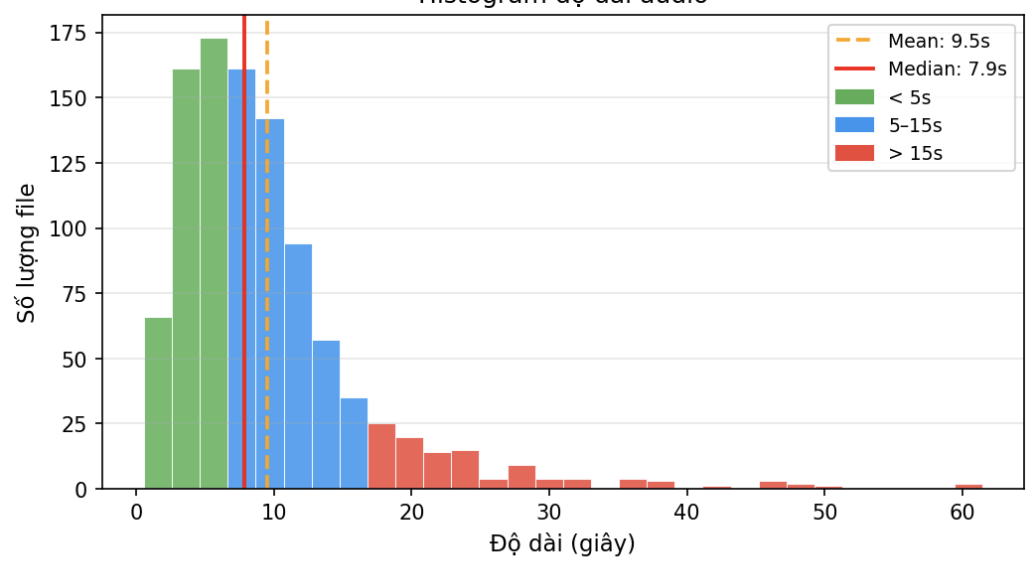
\includegraphics[width=0.82\textwidth]{report_figures/image1.png}
    \caption{Phân bố độ dài audio trong tập đánh giá}
    \label{fig:audio-duration-distribution}
\end{figure}

Hình~\ref{fig:audio-duration-distribution} cho thấy phần lớn các mẫu audio trong tập đánh giá có độ dài ngắn đến trung bình, tập trung chủ yếu quanh vùng dưới 15 giây. Giá trị trung bình khoảng 9.56 giây và trung vị khoảng 7.95 giây, cho thấy tập đánh giá phản ánh khá đúng kiểu câu hỏi thoại ngắn trong một hệ thống tư vấn. Tuy nhiên, phân bố vẫn có một số mẫu dài hơn 15 giây, thậm chí kéo dài tới khoảng một phút. Nhóm mẫu dài này quan trọng vì chúng giúp kiểm tra khả năng xử lý của ASR và pipeline streaming trong các trường hợp người dùng nói dài, đặt câu hỏi phức tạp hoặc mô tả nhiều điều kiện sức khỏe cùng lúc.

\section{Độ đo}

Các thực nghiệm sử dụng ba nhóm độ đo chính: chất lượng nội dung của RAG, tốc độ của ASR và độ trễ cùng chất lượng nghe của TTS streaming. Việc tách độ đo theo từng nhóm giúp phân biệt lỗi do truy xuất, lỗi do nhận dạng tiếng nói và độ chậm của quá trình tổng hợp âm thanh.

Với RAG, hệ thống được đánh giá bằng RAGAS, tập trung vào quan hệ giữa câu hỏi, câu trả lời tham chiếu, câu trả lời do hệ thống sinh và ngữ cảnh truy xuất. Quá trình đánh giá sử dụng bốn chỉ số:

\begin{itemize}
    \item \textbf{Answer Correctness:} mức độ câu trả lời của hệ thống phù hợp với câu trả lời tham chiếu.
    \item \textbf{Faithfulness:} mức độ câu trả lời bám sát ngữ cảnh được truy xuất.
    \item \textbf{Context Recall:} mức độ ngữ cảnh truy xuất bao phủ thông tin cần thiết trong câu trả lời tham chiếu.
    \item \textbf{Context Precision:} mức độ các đoạn văn bản được truy xuất thực sự liên quan và được xếp hạng phù hợp.
\end{itemize}

Với ASR, hai nhóm độ đo được sử dụng là Word Error Rate và real-time factor. Word Error Rate phản ánh mức sai khác giữa transcript sinh ra và transcript tham chiếu. Real-time factor phản ánh tốc độ xử lý so với thời lượng audio đầu vào; nếu real-time factor nhỏ hơn 1, mô hình xử lý nhanh hơn thời lượng audio thực.

Với TTS streaming, chỉ số quan trọng nhất là Time-to-First-Audio, tức thời gian từ khi mô-đun xử lý hội thoại bắt đầu sinh phản hồi đến khi người dùng nghe được phần âm thanh đầu tiên. Ngoài ra, tổng thời gian phản hồi và các percentile như p50, p90 được dùng để phản ánh cả trải nghiệm điển hình và các trường hợp chậm.

\section{Đánh giá TTS}

TTS được đánh giá theo hai nhóm tiêu chí: độ trễ khi tham gia pipeline streaming và chất lượng nghe chủ quan của âm thanh sinh ra. Về độ trễ, hệ thống đo Time-to-First-Audio khi thay đổi kích thước đoạn văn bản gửi sang TTS. Về chất lượng nghe, đồ án sử dụng bảng chấm MOS nội bộ trên ba tiêu chí: độ tự nhiên của giọng đọc, ngữ điệu và độ liền mạch giữa các đoạn âm thanh.

Thí nghiệm được thực hiện trên bốn cấu hình: không chia đoạn, chia đoạn theo ngưỡng 80 ký tự, 40 ký tự và 20 ký tự. Mỗi cấu hình gồm 250 lượt đo. Kết quả thống kê cho thấy việc chia văn bản thành các đoạn ngắn hơn giúp giảm mạnh thời gian tạo âm thanh đầu tiên so với phương án chờ toàn bộ câu trả lời. Bảng~\ref{tab:latency-chunk-results} tóm tắt một số kết quả chính:

\begin{table}[H]
    \centering
    \begin{tabular}{|p{2.5cm}|R{2cm}|R{2.5cm}|R{2.5cm}|R{2.5cm}|}
        \hline
        \textbf{Cấu hình} & \textbf{Số mẫu} & \textbf{TTFA mean (ms)} & \textbf{TTFA p50 (ms)} & \textbf{TTFA p90 (ms)} \\
        \hline
        Không chia đoạn   & 250             & \textbf{1614.2}         & \textbf{1523.0}        & \textbf{1760.9}        \\
        \hline
        80 ký tự          & 250             & 1059.5                  & 1055.1                 & 1179.4                 \\
        \hline
        40 ký tự          & 250             & 748.8                   & 746.7                  & 821.6                  \\
        \hline
        20 ký tự          & 250             & 603.9                   & 603.4                  & 660.0                  \\
        \hline
    \end{tabular}
    \caption{Kết quả đánh giá độ trễ TTS streaming theo cấu hình chia đoạn}
    \label{tab:latency-chunk-results}
\end{table}

Kết quả này cho thấy chiến thuật streaming có tác động rõ rệt đến độ trễ cảm nhận. Cấu hình không chia đoạn có p50 khoảng 1523 ms, gần sát ngưỡng mục tiêu 1.5 giây và có p90 vượt ngưỡng. Khi giảm kích thước đoạn xuống 40 ký tự, p50 TTFA giảm còn khoảng 747 ms và p90 còn khoảng 822 ms. Với cấu hình 20 ký tự, TTFA tiếp tục giảm nhưng có nguy cơ làm tiếng nói bị ngắt đoạn nhiều hơn. Vì vậy, ngưỡng 40 ký tự là lựa chọn cân bằng hơn giữa độ trễ và độ tự nhiên của audio trong hệ thống hiện tại.

Ngoài TTFA, tổng thời gian xử lý cũng giảm khi dùng chia đoạn. Trung bình cấu hình không chia đoạn cần khoảng 4333.5 ms, trong khi cấu hình 40 ký tự cần khoảng 1508.9 ms và cấu hình 20 ký tự cần khoảng 1258.8 ms. Điều này phản ánh lợi ích của việc chồng lấp thời gian sinh văn bản và thời gian tổng hợp tiếng nói. Tuy nhiên, giảm kích thước đoạn cũng có thể làm giảm độ liền mạch của giọng đọc, nên cần đối chiếu kết quả độ trễ với đánh giá MOS nội bộ.

Bên cạnh độ trễ, bảng~\ref{tab:tts-mos-results} trình bày kết quả chấm nghe chủ quan dạng MOS nội bộ trên 250 mẫu. Ba tiêu chí được sử dụng gồm Naturalness, Prosody và Continuity. Naturalness phản ánh mức độ tự nhiên tổng thể của giọng đọc; Prosody phản ánh ngữ điệu, nhấn nhá và lên xuống giọng; Continuity phản ánh mức độ liền mạch giữa các đoạn âm thanh sau khi chia văn bản.

\begin{table}[H]
    \centering
    \begin{tabular}{|p{3.2cm}|R{2.6cm}|R{2.3cm}|R{2.5cm}|R{2.4cm}|}
        \hline
        \textbf{Cấu hình} & \textbf{Naturalness} & \textbf{Prosody} & \textbf{Continuity} & \textbf{Trung bình} \\
        \hline
        Không chia đoạn   & \textbf{4.248}       & \textbf{4.376}   & \textbf{4.468}      & \textbf{4.364}      \\
        \hline
        80 ký tự          & 4.052                & 3.816            & 4.068               & 3.979               \\
        \hline
        40 ký tự          & 3.752                & 3.688            & 3.736               & 3.725               \\
        \hline
        20 ký tự          & 3.312                & 3.216            & 3.256               & 3.261               \\
        \hline
    \end{tabular}
    \caption{Kết quả đánh giá MOS nội bộ của TTS theo cấu hình chia đoạn}
    \label{tab:tts-mos-results}
\end{table}

Kết quả MOS cho thấy cấu hình không chia đoạn có chất lượng nghe cao nhất, vì câu trả lời được tổng hợp như một đoạn liên tục và ít bị ảnh hưởng bởi ranh giới chia văn bản. Tuy nhiên, cấu hình này có Time-to-First-Audio cao nhất. Ngược lại, cấu hình 20 ký tự đạt độ trễ thấp nhất nhưng điểm MOS giảm rõ rệt, đặc biệt ở ngữ điệu và độ liền mạch. Cấu hình 40 ký tự không đạt chất lượng nghe tốt nhất, nhưng giữ điểm trung bình ở mức chấp nhận được trong khi giảm mạnh TTFA. Do đó, cấu hình này được lựa chọn như một điểm cân bằng giữa trải nghiệm nghe và độ trễ phản hồi.

\section{Đánh giá RAG}

Framework đánh giá chất lượng được xây dựng quanh RAGAS \cite{ragas}. Bộ dữ liệu đánh giá gồm câu hỏi, câu trả lời tham chiếu và ngữ cảnh liên quan. Với mỗi mẫu, pipeline sử dụng Qwen-3-4b-2507 để sinh câu trả lời và lưu lại các đoạn văn bản được truy xuất. Sau đó, Gemini 2.5 Pro được gọi qua API với vai trò mô hình đánh giá để tính Answer Correctness, Faithfulness, Context Recall và Context Precision \cite{gemini25}. Việc tách hai vai trò giúp kết quả đánh giá không bị hiểu nhầm là câu trả lời của hệ thống được sinh bởi Gemini.

Bảng~\ref{tab:ragas-retrieval-results} trình bày kết quả đánh giá RAGAS trên 600 mẫu. Câu trả lời được sinh bởi Qwen-3-4b-2507, còn bốn chỉ số được chấm bằng Gemini 2.5 Pro thông qua API. Ba cấu hình được so sánh theo số lượng đoạn văn bản ứng viên ban đầu và số đoạn tốt nhất được đưa vào đầu vào của Qwen-3-4b-2507.

\begin{table}[H]
    \centering
    \begin{tabular}{|p{3.2cm}|R{2.6cm}|R{2.5cm}|R{2.5cm}|R{2.5cm}|}
        \hline
        \textbf{Cấu hình truy xuất}   & \textbf{Answer Correctness} & \textbf{Faithfulness} & \textbf{Context Recall} & \textbf{Context Precision} \\
        \hline
        10 đoạn ứng viên, chọn 3 đoạn & 0.5887                      & 0.7375                & 0.5184                  & 0.5426                     \\
        \hline
        15 đoạn ứng viên, chọn 5 đoạn & 0.6098                      & 0.7723                & 0.6239                  & \textbf{0.5709}            \\
        \hline
        20 đoạn ứng viên, chọn 7 đoạn & \textbf{0.6136}             & \textbf{0.7897}       & \textbf{0.6830}         & 0.5493                     \\
        \hline
    \end{tabular}
    \caption{Kết quả đánh giá chất lượng RAG theo cấu hình truy xuất}
    \label{tab:ragas-retrieval-results}
\end{table}

Kết quả cho thấy khi tăng số lượng đoạn ứng viên và số đoạn được đưa vào LLM, context recall và faithfulness có xu hướng tăng. Tuy nhiên, context precision không tăng đơn điệu: cấu hình 20 đoạn ứng viên, chọn 7 đoạn có recall cao hơn nhưng precision thấp hơn cấu hình 15 đoạn ứng viên, chọn 5 đoạn. Điều này cho thấy việc đưa thêm ngữ cảnh không luôn làm câu trả lời tốt hơn; hệ thống cần cân bằng giữa độ phủ tài liệu, độ nhiễu của context và chi phí latency. Trong phạm vi đồ án, cấu hình 15 đoạn ứng viên, chọn 5 đoạn được xem là điểm cân bằng hợp lý giữa chất lượng truy xuất và độ trễ cho voicebot.

Phần phân tích thời gian xử lý RAG tập trung vào ảnh hưởng của số lượng đoạn ứng viên và số đoạn được đưa vào đầu vào của LLM. Ba cấu hình truy xuất được so sánh theo thời gian RAG và thời gian sinh phần trả lời đầu tiên của LLM.

\begin{figure}[H]
    \centering
    \begin{subfigure}{0.7\textwidth}
        \centering
        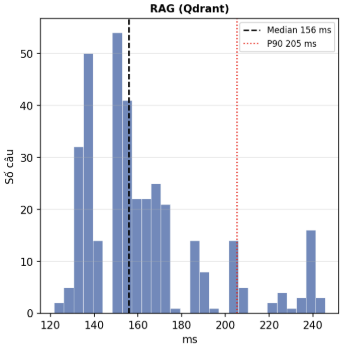
\includegraphics[width=\textwidth]{report_figures/image4_rag.png}
        \caption{Thời gian RAG (mở rộng truy vấn, truy xuất và reranking)}
    \end{subfigure}

    \vspace{0.4em}

    \begin{subfigure}{0.7\textwidth}
        \centering
        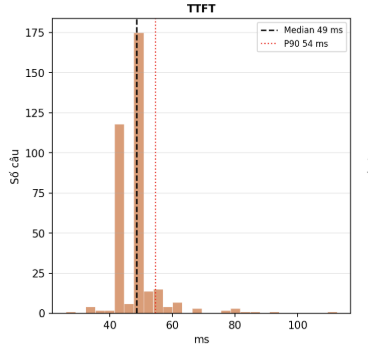
\includegraphics[width=\textwidth]{report_figures/image4_ttft.png}
        \caption{Thời gian sinh phần trả lời đầu tiên của LLM (TTFT)}
    \end{subfigure}
    \caption{Phân bố thời gian RAG và TTFT với cấu hình lấy 10 đoạn ứng viên, chọn 3 đoạn}
    \label{fig:rag-ttft-10-3}
\end{figure}

\begin{figure}[H]
    \centering
    \begin{subfigure}{0.7\textwidth}
        \centering
        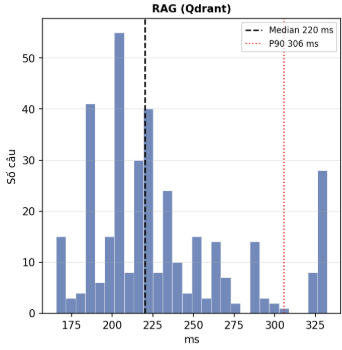
\includegraphics[width=\textwidth]{report_figures/image5_rag.png}
        \caption{Thời gian RAG (mở rộng truy vấn, truy xuất và reranking)}
    \end{subfigure}

    \vspace{0.4em}

    \begin{subfigure}{0.7\textwidth}
        \centering
        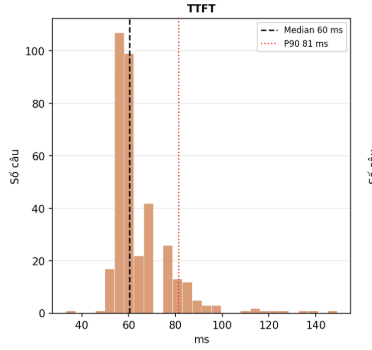
\includegraphics[width=\textwidth]{report_figures/image5_ttft.png}
        \caption{Thời gian sinh phần trả lời đầu tiên của LLM (TTFT)}
    \end{subfigure}
    \caption{Phân bố thời gian RAG và TTFT với cấu hình lấy 15 đoạn ứng viên, chọn 5 đoạn}
    \label{fig:rag-ttft-15-5}
\end{figure}

\begin{figure}[H]
    \centering
    \begin{subfigure}{0.7\textwidth}
        \centering
        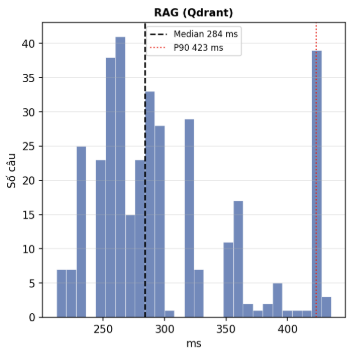
\includegraphics[width=\textwidth]{report_figures/image6_rag.png}
        \caption{Thời gian RAG (mở rộng truy vấn, truy xuất và reranking)}
    \end{subfigure}

    \vspace{0.4em}

    \begin{subfigure}{0.7\textwidth}
        \centering
        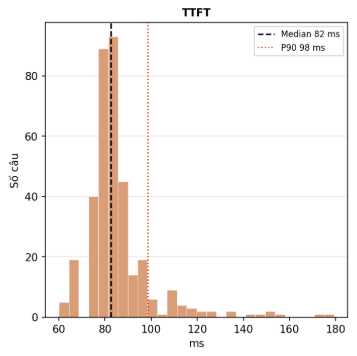
\includegraphics[width=\textwidth]{report_figures/image6_ttft.png}
        \caption{Thời gian sinh phần trả lời đầu tiên của LLM (TTFT)}
    \end{subfigure}
    \caption{Phân bố thời gian RAG và TTFT với cấu hình lấy 20 đoạn ứng viên, chọn 7 đoạn}
    \label{fig:rag-ttft-20-7}
\end{figure}

Hình~\ref{fig:rag-ttft-10-3}, Hình~\ref{fig:rag-ttft-15-5} và Hình~\ref{fig:rag-ttft-20-7} minh họa ảnh hưởng của cấu hình truy xuất đến thời gian xử lý của khối LLM/RAG. Mỗi cấu hình gồm hai nhóm thời gian chính: thời gian RAG, tức thời gian mở rộng truy vấn, truy xuất và reranking; và thời gian sinh phần trả lời đầu tiên của LLM. Khi tăng số lượng đoạn ứng viên và số đoạn đưa vào LLM, thời gian RAG có xu hướng tăng vì hệ thống phải xử lý nhiều ứng viên hơn ở bước reranking và đưa nhiều ngữ cảnh hơn vào prompt. Ngược lại, thời gian sinh phần trả lời đầu tiên của LLM biến động ít hơn, do phần này phụ thuộc nhiều vào backend LLM và độ dài prompt sau khi đã chọn context.

Các kết quả trong Hình~\ref{fig:rag-ttft-10-3}, Hình~\ref{fig:rag-ttft-15-5} và Hình~\ref{fig:rag-ttft-20-7} giúp giải thích lý do đồ án không chỉ chọn cấu hình có nhiều tài liệu nhất. Cấu hình truy xuất lớn hơn có thể cải thiện độ phủ ngữ cảnh, nhưng cũng làm tăng độ trễ trước khi LLM bắt đầu sinh câu trả lời. Vì voicebot cần phản hồi nhanh, cấu hình truy xuất phải cân bằng giữa chất lượng RAG và độ trễ cảm nhận của người dùng.

Bên cạnh chất lượng RAG, đồ án đánh giá ASR bằng WER và real-time factor, đồng thời đo ảnh hưởng của chiến thuật TTS streaming tới thời gian tạo âm thanh đầu tiên. Chất lượng cảm nhận của TTS được đánh giá bằng bảng MOS nội bộ để phân tích quan hệ giữa kích thước đoạn, độ trễ và độ tự nhiên của audio. Việc tách các chỉ số theo mô-đun giúp xác định thành phần nào là nút thắt trong từng cấu hình.

\section{Đánh giá ASR}

ASR được đánh giá theo hai khía cạnh: độ chính xác của transcript và tốc độ xử lý. Độ chính xác được đo bằng WER trên tập audio có transcript tham chiếu. Tốc độ được đo bằng real-time factor để xác định mô hình có đủ nhanh cho hệ thống hội thoại thời gian thực hay không.

\begin{figure}[H]
    \centering
    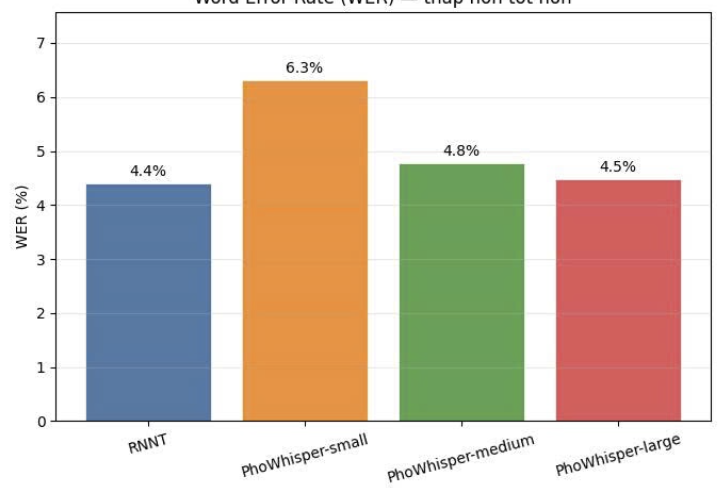
\includegraphics[width=0.48\textwidth]{report_figures/asr_wer_model_comparison.png}
    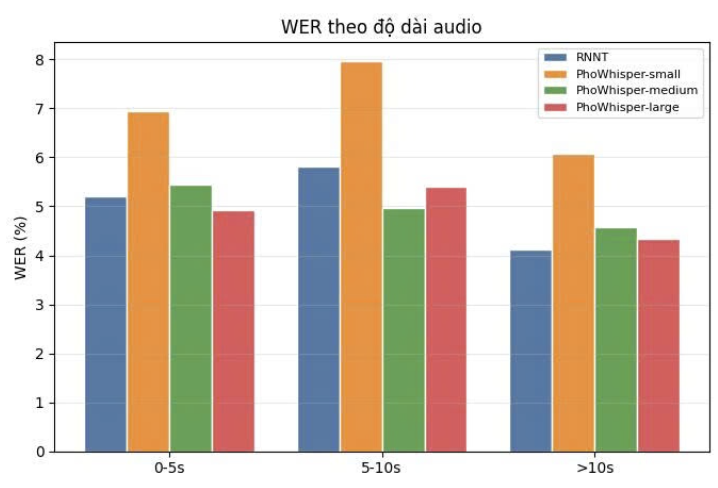
\includegraphics[width=0.48\textwidth]{report_figures/asr_wer_duration_comparison.png}
    \caption{So sánh WER của các mô hình ASR theo mô hình và theo độ dài audio}
    \label{fig:asr-wer-comparison}
\end{figure}

Hình~\ref{fig:asr-wer-comparison} so sánh lỗi nhận dạng tiếng nói của nhiều mô hình ASR trên tập đánh giá tiếng Việt. Kết quả tổng thể cho thấy RNNT đạt WER khoảng 4.4\%, PhoWhisper-small khoảng 6.3\%, PhoWhisper-medium khoảng 4.8\% và PhoWhisper-large khoảng 4.5\%. Khi phân tích theo độ dài audio, WER thay đổi giữa các nhóm 0--5 giây, 5--10 giây và trên 10 giây, cho thấy chất lượng ASR không chỉ phụ thuộc vào mô hình mà còn phụ thuộc vào đặc điểm câu nói. Điều này phản ánh đặc điểm quan trọng của pipeline voicebot: transcript đầu vào không phải lúc nào cũng hoàn hảo, và lỗi ASR có thể lan truyền sang bước truy xuất tri thức. Vì vậy, hệ thống cần có các bước giảm tác động của lỗi nhận dạng, chẳng hạn chuẩn hóa thuật ngữ dinh dưỡng, query expansion và truy xuất dựa trên nhiều biến thể câu hỏi.

\begin{figure}[H]
    \centering
    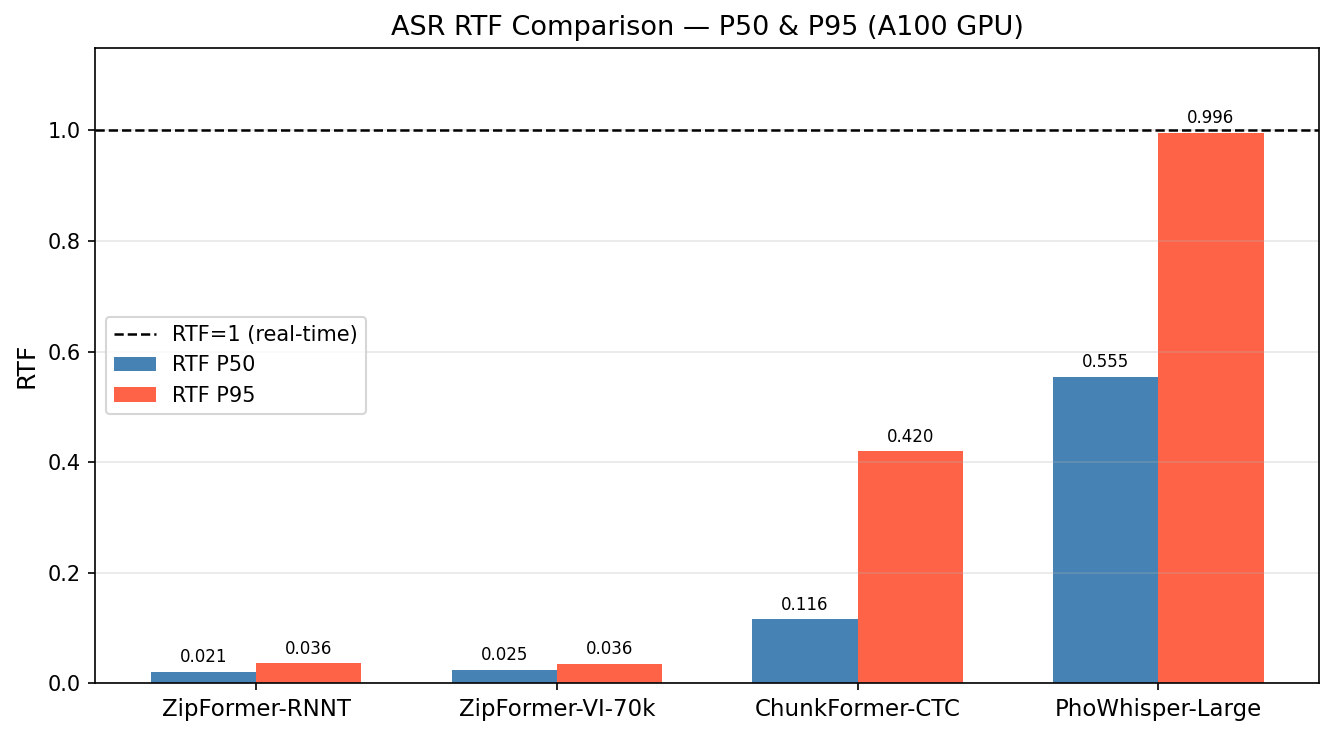
\includegraphics[width=0.82\textwidth]{report_figures/asr_rtf_bar_comparison.png}
    \caption{So sánh real-time factor của các mô hình ASR}
    \label{fig:asr-rtf-comparison}
\end{figure}

Hình~\ref{fig:asr-rtf-comparison} cho thấy sự khác biệt rõ giữa các mô hình ASR về tốc độ xử lý. Đường tham chiếu RTF bằng 1 biểu thị ngưỡng real-time: nếu RTF nhỏ hơn 1, mô hình xử lý nhanh hơn thời lượng audio đầu vào. ZipFormer-RNNT và ZipFormer-VI-70k có RTF rất thấp ở cả p50 và p95, cho thấy khả năng xử lý nhanh và ổn định hơn cho bài toán hội thoại thời gian thực. ChunkFormer-CTC vẫn nằm dưới ngưỡng real-time nhưng có p95 cao hơn, nghĩa là trong một số trường hợp chậm hệ thống có thể mất nhiều thời gian hơn. PhoWhisper-Large có p95 gần 1, tức là các trường hợp chậm gần sát ngưỡng real-time. Kết quả này cho thấy lựa chọn mô hình ASR ảnh hưởng trực tiếp đến độ trễ đầu vào của toàn bộ pipeline.

\chapter{KẾT LUẬN VÀ HƯỚNG PHÁT TRIỂN}

\section{Đóng góp chính của đồ án}

Đồ án đề xuất và hiện thực một hệ thống tư vấn dinh dưỡng tiếng Việt có khả năng tương tác hai chiều bằng tiếng nói. Thay vì chỉ ghép nối tuần tự các mô hình có sẵn, giải pháp tập trung giải quyết đồng thời hai yêu cầu của một voicebot sử dụng RAG: câu trả lời phải dựa trên kho tri thức có kiểm soát và phần âm thanh đầu tiên phải được tạo đủ sớm để duy trì cảm giác hội thoại.

Đóng góp thứ nhất là xây dựng một pipeline hoàn chỉnh từ tiếng nói đầu vào đến tiếng nói phản hồi. Hệ thống gồm giao diện, Gateway điều phối phiên, mô-đun ASR, mô-đun xử lý hội thoại, Qwen-3-4b-2507, mô-đun TTS, Qdrant và Redis. Pipeline hỗ trợ phát hiện lượt nói bằng VAD, nhận dạng tiếng Việt, truy xuất tri thức, sinh câu trả lời theo luồng, tổng hợp âm thanh theo từng phần và barge-in khi người dùng ngắt lời. Các thành phần được đóng gói bằng Docker và có thể được chạy để kiểm thử trực tiếp trên giao diện.

Đóng góp thứ hai là xây dựng quy trình RAG cho chủ đề dinh dưỡng tiếng Việt. Kho tri thức được tạo từ 1060 bài viết thuộc các nguồn có tính chuyên môn, sau đó được làm sạch, phân đoạn và mã hóa bằng mô hình embedding tiếng Việt. Ở thời điểm truy vấn, hệ thống chuẩn hóa một số cách diễn đạt thường gặp, lấy một tập đoạn văn bản ứng viên từ Qdrant và sử dụng mô hình rerank để chọn tập ngữ cảnh nhỏ hơn. Năm đoạn phù hợp nhất được đưa vào prompt của Qwen-3-4b-2507. Guardrail dựa trên luật và kiểm tra mức đủ tối thiểu của bằng chứng được sử dụng để hạn chế một số câu hỏi ngoài phạm vi, yêu cầu chẩn đoán, điều chỉnh thuốc hoặc trường hợp không có đủ nội dung truy xuất.

Đóng góp thứ ba là tổ chức cơ chế streaming chồng lấp giữa quá trình sinh văn bản và tổng hợp tiếng nói. Thay vì chờ Qwen-3-4b-2507 sinh xong toàn bộ câu trả lời, Gateway tích lũy văn bản đến một ranh giới phù hợp rồi chuyển từng đoạn sang VieNeu-TTS. Trong khi TTS tổng hợp đoạn hiện tại, Qwen-3-4b-2507 tiếp tục sinh đoạn tiếp theo. Phương pháp này không làm giảm tổng lượng tính toán của các mô hình, nhưng rút ngắn khoảng im lặng trước khi người dùng nghe được phản hồi.

Đóng góp thứ tư là xây dựng quy trình thực nghiệm cho cả chất lượng nội dung và độ trễ. Ba cấu hình truy xuất được so sánh bằng Answer Correctness, Faithfulness, Context Recall và Context Precision. Câu trả lời được sinh bởi Qwen-3-4b-2507, còn các chỉ số RAGAS được chấm bằng Gemini 2.5 Pro qua API. Kết quả cho thấy cấu hình lấy 15 đoạn ứng viên và chọn 5 đoạn đạt Answer Correctness 0,6098, Faithfulness 0,7723, Context Recall 0,6239 và Context Precision 0,5709. Cấu hình này được lựa chọn làm điểm cân bằng giữa độ phủ của ngữ cảnh, lượng nhiễu đưa vào prompt và chi phí xử lý.

Đối với độ trễ, thực nghiệm cho thấy việc chia luồng văn bản có ảnh hưởng trực tiếp đến Time-to-First-Audio. Khi chuyển từ phương án chờ toàn bộ câu trả lời sang cấu hình đoạn 40 ký tự, trung vị Time-to-First-Audio giảm từ khoảng 1523 ms xuống 747 ms và phân vị p90 giảm xuống khoảng 822 ms. Cấu hình 20 ký tự tiếp tục giảm độ trễ nhưng làm tăng nguy cơ câu nói bị chia nhỏ và thiếu tự nhiên. Vì vậy, ngưỡng 40 ký tự được lựa chọn như một cấu hình phù hợp hơn cho hệ thống hiện tại.

\section{Kết luận}

Kết quả của đồ án cho thấy chất lượng của một hệ thống hỏi đáp qua tiếng nói không chỉ phụ thuộc vào từng mô hình ASR, LLM hoặc TTS riêng lẻ. Trải nghiệm cuối cùng được quyết định bởi cách các thành phần trao đổi dữ liệu, cách ngữ cảnh được lựa chọn và thời điểm hệ thống bắt đầu phát âm thanh. Một mô hình có tốc độ tốt vẫn có thể tạo ra trải nghiệm chậm nếu toàn bộ pipeline được thực hiện tuần tự.

Phát hiện quan trọng thứ nhất là tăng số lượng ngữ cảnh không luôn cải thiện đồng thời mọi chỉ số. Cấu hình lấy 20 đoạn ứng viên và chọn 7 đoạn đạt Context Recall và Faithfulness cao hơn, nhưng Context Precision thấp hơn cấu hình 15 đoạn ứng viên và chọn 5 đoạn. Điều này cho thấy ngữ cảnh lớn hơn có thể tăng độ phủ nhưng cũng đưa thêm nội dung ít liên quan vào prompt. Đối với voicebot, cấu hình truy xuất cần được lựa chọn dựa trên cả chất lượng và độ trễ, thay vì chỉ tối đa hóa số lượng tài liệu.

Phát hiện thứ hai là Time-to-First-Audio có thể được cải thiện đáng kể ở tầng tổ chức hệ thống mà không cần thay đổi mô hình nền. Việc chồng lấp quá trình sinh văn bản và tổng hợp âm thanh giúp người dùng nghe được phản hồi sớm hơn, mặc dù toàn bộ câu trả lời chưa được hoàn thành. Tuy nhiên, kích thước đoạn quá nhỏ làm tăng số lần gọi TTS và có thể phá vỡ nhịp điệu của câu nói. Do đó, tối ưu độ trễ của voicebot là một bài toán cân bằng giữa tốc độ và tính tự nhiên, không phải chỉ là giảm một tham số xuống mức nhỏ nhất.

Phát hiện thứ ba là lỗi và độ trễ có tính tích lũy theo pipeline. Transcript không chính xác có thể làm sai truy vấn; truy vấn sai làm giảm chất lượng tài liệu; ngữ cảnh không phù hợp tiếp tục ảnh hưởng đến câu trả lời và tiếng nói đầu ra. Vì vậy, các bước chuẩn hóa truy vấn, reranking, kiểm tra bằng chứng và ghi nhận thời gian theo từng thành phần có ý nghĩa thực tế hơn việc chỉ đánh giá câu trả lời cuối cùng.

Bài học quan trọng rút ra từ quá trình thực hiện là cần phân biệt rõ giữa khả năng của mô hình và khả năng của hệ thống. Đồ án không huấn luyện lại các mô hình nền, nhưng đóng góp nằm ở việc lựa chọn, kết nối, kiểm soát và đánh giá chúng trong một bài toán cụ thể. Một hệ thống có thể sử dụng các mô hình có sẵn nhưng vẫn cần giải quyết các vấn đề kỹ thuật về dữ liệu, quản lý phiên, streaming, barge-in, truy xuất, cache và tái lập môi trường triển khai.

Hệ thống hiện tại đã hoàn thành được luồng hỏi đáp bằng tiếng nói trên giao diện và tạo ra một nền tảng có thể tiếp tục thử nghiệm. Tuy nhiên, kết quả chưa đại diện cho một sản phẩm tư vấn y tế hoàn chỉnh. Guardrail hiện chủ yếu dựa trên luật, kho tri thức còn giới hạn và kết quả thực nghiệm phụ thuộc vào phần cứng cũng như tập dữ liệu đánh giá. Các giới hạn này cần được xem xét khi diễn giải kết quả và khi đưa hệ thống vào môi trường thực tế.

\section{Hướng phát triển}

Hướng cải thiện gần nhất là nâng cao độ tin cậy của nội dung. Kho tri thức cần được cập nhật định kỳ, bổ sung cơ chế quản lý phiên bản và kiểm duyệt tài liệu trước khi nạp vào Qdrant. Hệ thống có thể bổ sung bộ phân loại rủi ro cho câu hỏi đầu vào, kiểm tra mức đủ bằng chứng chặt chẽ hơn và cơ chế từ chối trả lời khi tài liệu truy xuất không hỗ trợ kết luận. Việc hiển thị nguồn tham khảo trên giao diện cũng giúp người dùng kiểm tra nội dung thay vì chỉ nhận câu trả lời bằng tiếng nói.

Về truy xuất, có thể nghiên cứu kết hợp truy xuất từ khóa với truy xuất vector để xử lý tốt hơn tên chất dinh dưỡng, bệnh lý và thuật ngữ cụ thể. Các tham số như số đoạn ứng viên, số đoạn sau rerank và kích thước đoạn tài liệu có thể được điều chỉnh theo loại câu hỏi thay vì sử dụng một cấu hình cố định. Exact cache và semantic cache cũng cần được đánh giá bằng tỷ lệ cache hit, thời gian tiết kiệm và nguy cơ dùng lại ngữ cảnh không phù hợp.

Về xử lý tiếng nói, hệ thống cần được kiểm thử với tiếng ồn, nhiều vùng giọng, tốc độ nói khác nhau và câu hỏi dài. ASR có thể được cải thiện bằng cơ chế nhận dạng theo luồng thực sự hoặc bước hiệu chỉnh transcript dựa trên từ vựng dinh dưỡng. Đối với TTS, đánh giá MOS nội bộ cần được mở rộng với nhiều người nghe hơn, quy trình chấm độc lập hơn và nhiều điều kiện âm thanh hơn để kết luận về quan hệ giữa kích thước đoạn, độ trễ và độ tự nhiên có độ tin cậy cao hơn.

Về khả năng vận hành, cần tiến hành kiểm thử đồng thời với nhiều phiên để xác định giới hạn của ASR, Qwen-3-4b-2507 và VieNeu-TTS trên phần cứng cụ thể. Các chỉ số nên bao gồm Time-to-First-Audio theo p50 và p90, tỷ lệ yêu cầu thành công, độ dài hàng đợi, mức sử dụng CPU/GPU và khả năng giữ dữ liệu tách biệt giữa các phiên. Kết quả này là cơ sở để lựa chọn giới hạn đồng thời, cơ chế xếp hàng hoặc số tiến trình phù hợp.

Về mở rộng ứng dụng, hệ thống có thể bổ sung xác thực người dùng và cơ sở dữ liệu quan hệ để lưu hồ sơ, mục tiêu dinh dưỡng, lịch sử sử dụng và phản hồi. Các dữ liệu cá nhân cần được tách khỏi Qdrant, kiểm soát quyền truy cập và chỉ được sử dụng khi người dùng đồng ý. Khi có dữ liệu sử dụng thực tế, hệ thống có thể phát hiện các khoảng trống của kho tri thức, bổ sung câu hỏi thường gặp và đánh giá lại pipeline theo nhu cầu thực tế thay vì chỉ dựa trên tập kiểm thử xây dựng trước.

\begin{thebibliography}{99}
    \bibitem{rnnt}
    Alex Graves. Sequence Transduction with Recurrent Neural Networks. arXiv:1211.3711, 2012. \url{https://arxiv.org/abs/1211.3711}

    \bibitem{conformer}
    Anmol Gulati et al. Conformer: Convolution-augmented Transformer for Speech Recognition. Interspeech, 2020. \url{https://arxiv.org/abs/2005.08100}

    \bibitem{zipformer}
    Zengwei Yao et al. Zipformer: A Faster and Better Encoder for Automatic Speech Recognition. ICLR, 2024. \url{https://arxiv.org/abs/2310.11230}

    \bibitem{zipformer6000h}
    hynt. Vietnamese Speech-to-Text (ASR) -- ZipFormer-30M-RNNT-6000h. Hugging Face model card. \url{https://huggingface.co/hynt/Zipformer-30M-RNNT-6000h}

    \bibitem{transformer}
    Ashish Vaswani et al. Attention Is All You Need. NeurIPS, 2017. \url{https://arxiv.org/abs/1706.03762}

    \bibitem{qwen3}
    Qwen Team. Qwen3 Technical Report. arXiv:2505.09388, 2025. \url{https://arxiv.org/abs/2505.09388}

    \bibitem{qwen3modelcard}
    Qwen Team. Qwen3-4B-Instruct-2507 Model Card. Hugging Face. \url{https://huggingface.co/Qwen/Qwen3-4B-Instruct-2507}

    \bibitem{rag}
    Patrick Lewis et al. Retrieval-Augmented Generation for Knowledge-Intensive NLP Tasks. NeurIPS, 2020. \url{https://arxiv.org/abs/2005.11401}

    \bibitem{hyde}
    Luyu Gao, Xueguang Ma, Jimmy Lin, Jamie Callan. Precise Zero-Shot Dense Retrieval without Relevance Labels. ACL, 2023. \url{https://arxiv.org/abs/2212.10496}

    \bibitem{sbert}
    Nils Reimers, Iryna Gurevych. Sentence-BERT: Sentence Embeddings using Siamese BERT-Networks. EMNLP-IJCNLP, 2019. \url{https://arxiv.org/abs/1908.10084}

    \bibitem{hnsw}
    Yu. A. Malkov, D. A. Yashunin. Efficient and Robust Approximate Nearest Neighbor Search using Hierarchical Navigable Small World Graphs. IEEE TPAMI, 2020. \url{https://arxiv.org/abs/1603.09320}

    \bibitem{ragas}
    Shahul Es, Jithin James, Luis Espinosa-Anke, Steven Schockaert. RAGAS: Automated Evaluation of Retrieval Augmented Generation. arXiv:2309.15217, 2023. \url{https://arxiv.org/abs/2309.15217}

    \bibitem{valle}
    Chengyi Wang et al. Neural Codec Language Models are Zero-Shot Text to Speech Synthesizers. arXiv:2301.02111, 2023. \url{https://arxiv.org/abs/2301.02111}

    \bibitem{vieneutts}
    Pham Nguyen Ngoc Bao. VieNeu-TTS: Vietnamese Text-to-Speech with Instant Voice Cloning. Hugging Face model card, 2026. \url{https://huggingface.co/pnnbao-ump/VieNeu-TTS}

    \bibitem{vieneutts03b}
    Pham Nguyen Ngoc Bao. VieNeu-TTS-0.3B: Ultra-Fast Vietnamese Text-to-Speech trained from scratch. Hugging Face model card, 2026. \url{https://huggingface.co/pnnbao-ump/VieNeu-TTS-0.3B}

    \bibitem{react}
    Meta Open Source. React Documentation. \url{https://react.dev/}

    \bibitem{vite}
    Vite Team. Vite Documentation. \url{https://vite.dev/guide/}

    \bibitem{webaudio}
    MDN Web Docs. Web Audio API. \url{https://developer.mozilla.org/en-US/docs/Web/API/Web_Audio_API}

    \bibitem{fastapi}
    Sebastián Ramírez. FastAPI Documentation: WebSockets. \url{https://fastapi.tiangolo.com/advanced/websockets/}

    \bibitem{sherpaonnx}
    k2-fsa. Sherpa-ONNX Documentation. \url{https://k2-fsa.github.io/sherpa/onnx/}

    \bibitem{silerovad}
    Silero Team. Silero VAD: pre-trained enterprise-grade Voice Activity Detector. GitHub repository. \url{https://github.com/snakers4/silero-vad}

    \bibitem{vietembedding}
    AITeamVN. Vietnamese Embedding. Hugging Face model card. \url{https://huggingface.co/AITeamVN/Vietnamese_Embedding}

    \bibitem{vietreranker}
    thanhtantran. Vietnamese Reranker. Hugging Face model card. \url{https://huggingface.co/thanhtantran/Vietnamese_Reranker}

    \bibitem{qdrant}
    Qdrant. Qdrant Documentation. \url{https://qdrant.tech/documentation/}

    \bibitem{redis}
    Redis. Redis Documentation. \url{https://redis.io/docs/latest/}

    \bibitem{dockercompose}
    Docker. Docker Compose Documentation. \url{https://docs.docker.com/compose/}

    \bibitem{cuda}
    NVIDIA. CUDA Toolkit Documentation. \url{https://docs.nvidia.com/cuda/}

    \bibitem{gemini25}
    Google DeepMind. Gemini 2.5: Our most intelligent AI model. \url{https://deepmind.google/technologies/gemini/}

\end{thebibliography}

\end{document}
